% Options for packages loaded elsewhere
\PassOptionsToPackage{unicode}{hyperref}
\PassOptionsToPackage{hyphens}{url}
%
\documentclass[
  Letterpaper,
]{scrbook}

\usepackage{amsmath,amssymb}
\usepackage{iftex}
\ifPDFTeX
  \usepackage[T1]{fontenc}
  \usepackage[utf8]{inputenc}
  \usepackage{textcomp} % provide euro and other symbols
\else % if luatex or xetex
  \usepackage{unicode-math}
  \defaultfontfeatures{Scale=MatchLowercase}
  \defaultfontfeatures[\rmfamily]{Ligatures=TeX,Scale=1}
\fi
\usepackage{lmodern}
\ifPDFTeX\else  
    % xetex/luatex font selection
    \setmainfont[]{Georgia}
\fi
% Use upquote if available, for straight quotes in verbatim environments
\IfFileExists{upquote.sty}{\usepackage{upquote}}{}
\IfFileExists{microtype.sty}{% use microtype if available
  \usepackage[]{microtype}
  \UseMicrotypeSet[protrusion]{basicmath} % disable protrusion for tt fonts
}{}
\makeatletter
\@ifundefined{KOMAClassName}{% if non-KOMA class
  \IfFileExists{parskip.sty}{%
    \usepackage{parskip}
  }{% else
    \setlength{\parindent}{0pt}
    \setlength{\parskip}{6pt plus 2pt minus 1pt}}
}{% if KOMA class
  \KOMAoptions{parskip=half}}
\makeatother
\usepackage{xcolor}
\usepackage[paperwidth=6in,paperheight=9in]{geometry}
\setlength{\emergencystretch}{3em} % prevent overfull lines
\setcounter{secnumdepth}{5}
% Make \paragraph and \subparagraph free-standing
\makeatletter
\ifx\paragraph\undefined\else
  \let\oldparagraph\paragraph
  \renewcommand{\paragraph}{
    \@ifstar
      \xxxParagraphStar
      \xxxParagraphNoStar
  }
  \newcommand{\xxxParagraphStar}[1]{\oldparagraph*{#1}\mbox{}}
  \newcommand{\xxxParagraphNoStar}[1]{\oldparagraph{#1}\mbox{}}
\fi
\ifx\subparagraph\undefined\else
  \let\oldsubparagraph\subparagraph
  \renewcommand{\subparagraph}{
    \@ifstar
      \xxxSubParagraphStar
      \xxxSubParagraphNoStar
  }
  \newcommand{\xxxSubParagraphStar}[1]{\oldsubparagraph*{#1}\mbox{}}
  \newcommand{\xxxSubParagraphNoStar}[1]{\oldsubparagraph{#1}\mbox{}}
\fi
\makeatother


\providecommand{\tightlist}{%
  \setlength{\itemsep}{0pt}\setlength{\parskip}{0pt}}\usepackage{longtable,booktabs,array}
\usepackage{calc} % for calculating minipage widths
% Correct order of tables after \paragraph or \subparagraph
\usepackage{etoolbox}
\makeatletter
\patchcmd\longtable{\par}{\if@noskipsec\mbox{}\fi\par}{}{}
\makeatother
% Allow footnotes in longtable head/foot
\IfFileExists{footnotehyper.sty}{\usepackage{footnotehyper}}{\usepackage{footnote}}
\makesavenoteenv{longtable}
\usepackage{graphicx}
\makeatletter
\newsavebox\pandoc@box
\newcommand*\pandocbounded[1]{% scales image to fit in text height/width
  \sbox\pandoc@box{#1}%
  \Gscale@div\@tempa{\textheight}{\dimexpr\ht\pandoc@box+\dp\pandoc@box\relax}%
  \Gscale@div\@tempb{\linewidth}{\wd\pandoc@box}%
  \ifdim\@tempb\p@<\@tempa\p@\let\@tempa\@tempb\fi% select the smaller of both
  \ifdim\@tempa\p@<\p@\scalebox{\@tempa}{\usebox\pandoc@box}%
  \else\usebox{\pandoc@box}%
  \fi%
}
% Set default figure placement to htbp
\def\fps@figure{htbp}
\makeatother
% definitions for citeproc citations
\NewDocumentCommand\citeproctext{}{}
\NewDocumentCommand\citeproc{mm}{%
  \begingroup\def\citeproctext{#2}\cite{#1}\endgroup}
\makeatletter
 % allow citations to break across lines
 \let\@cite@ofmt\@firstofone
 % avoid brackets around text for \cite:
 \def\@biblabel#1{}
 \def\@cite#1#2{{#1\if@tempswa , #2\fi}}
\makeatother
\newlength{\cslhangindent}
\setlength{\cslhangindent}{1.5em}
\newlength{\csllabelwidth}
\setlength{\csllabelwidth}{3em}
\newenvironment{CSLReferences}[2] % #1 hanging-indent, #2 entry-spacing
 {\begin{list}{}{%
  \setlength{\itemindent}{0pt}
  \setlength{\leftmargin}{0pt}
  \setlength{\parsep}{0pt}
  % turn on hanging indent if param 1 is 1
  \ifodd #1
   \setlength{\leftmargin}{\cslhangindent}
   \setlength{\itemindent}{-1\cslhangindent}
  \fi
  % set entry spacing
  \setlength{\itemsep}{#2\baselineskip}}}
 {\end{list}}
\usepackage{calc}
\newcommand{\CSLBlock}[1]{\hfill\break\parbox[t]{\linewidth}{\strut\ignorespaces#1\strut}}
\newcommand{\CSLLeftMargin}[1]{\parbox[t]{\csllabelwidth}{\strut#1\strut}}
\newcommand{\CSLRightInline}[1]{\parbox[t]{\linewidth - \csllabelwidth}{\strut#1\strut}}
\newcommand{\CSLIndent}[1]{\hspace{\cslhangindent}#1}

\makeatletter
\@ifpackageloaded{tcolorbox}{}{\usepackage[skins,breakable]{tcolorbox}}
\@ifpackageloaded{fontawesome5}{}{\usepackage{fontawesome5}}
\definecolor{quarto-callout-color}{HTML}{909090}
\definecolor{quarto-callout-note-color}{HTML}{0758E5}
\definecolor{quarto-callout-important-color}{HTML}{CC1914}
\definecolor{quarto-callout-warning-color}{HTML}{EB9113}
\definecolor{quarto-callout-tip-color}{HTML}{00A047}
\definecolor{quarto-callout-caution-color}{HTML}{FC5300}
\definecolor{quarto-callout-color-frame}{HTML}{acacac}
\definecolor{quarto-callout-note-color-frame}{HTML}{4582ec}
\definecolor{quarto-callout-important-color-frame}{HTML}{d9534f}
\definecolor{quarto-callout-warning-color-frame}{HTML}{f0ad4e}
\definecolor{quarto-callout-tip-color-frame}{HTML}{02b875}
\definecolor{quarto-callout-caution-color-frame}{HTML}{fd7e14}
\makeatother
\makeatletter
\@ifpackageloaded{bookmark}{}{\usepackage{bookmark}}
\makeatother
\makeatletter
\@ifpackageloaded{caption}{}{\usepackage{caption}}
\AtBeginDocument{%
\ifdefined\contentsname
  \renewcommand*\contentsname{Table of contents}
\else
  \newcommand\contentsname{Table of contents}
\fi
\ifdefined\listfigurename
  \renewcommand*\listfigurename{List of Figures}
\else
  \newcommand\listfigurename{List of Figures}
\fi
\ifdefined\listtablename
  \renewcommand*\listtablename{List of Tables}
\else
  \newcommand\listtablename{List of Tables}
\fi
\ifdefined\figurename
  \renewcommand*\figurename{Figure}
\else
  \newcommand\figurename{Figure}
\fi
\ifdefined\tablename
  \renewcommand*\tablename{Table}
\else
  \newcommand\tablename{Table}
\fi
}
\@ifpackageloaded{float}{}{\usepackage{float}}
\floatstyle{ruled}
\@ifundefined{c@chapter}{\newfloat{codelisting}{h}{lop}}{\newfloat{codelisting}{h}{lop}[chapter]}
\floatname{codelisting}{Listing}
\newcommand*\listoflistings{\listof{codelisting}{List of Listings}}
\makeatother
\makeatletter
\makeatother
\makeatletter
\@ifpackageloaded{caption}{}{\usepackage{caption}}
\@ifpackageloaded{subcaption}{}{\usepackage{subcaption}}
\makeatother

\usepackage{bookmark}

\IfFileExists{xurl.sty}{\usepackage{xurl}}{} % add URL line breaks if available
\urlstyle{same} % disable monospaced font for URLs
\hypersetup{
  pdftitle={Eyes on Health},
  pdfauthor={Richard Sprague},
  hidelinks,
  pdfcreator={LaTeX via pandoc}}


\title{Eyes on Health}
\author{Richard Sprague}
\date{2025-03-18}

\begin{document}
\frontmatter
\maketitle

\renewcommand*\contentsname{Table of contents}
{
\setcounter{tocdepth}{2}
\tableofcontents
}

\mainmatter
\bookmarksetup{startatroot}

\chapter*{Preface}\label{preface}
\addcontentsline{toc}{chapter}{Preface}

\markboth{Preface}{Preface}

The human eye has long captivated medical professionals as a unique
window into overall health. Through the delicate structures of the
retina, we can observe intricate networks of blood vessels, neural
tissue, and metabolic activity -- all without a single incision or
invasive procedure. This remarkable access point has made retinal
imaging, particularly fundus photography, an increasingly valuable tool
in health assessment and preventive care.

The convergence of high-resolution imaging technology and artificial
intelligence has revolutionized our ability to gather and interpret
retinal data. What was once the exclusive domain of ophthalmologists has
now become accessible to a broader range of health professionals,
opening new possibilities for early detection and monitoring of various
systemic conditions.

This book explores the science, application, and future potential of
fundus photography in clinical practice, with a particular focus on the
Opticare AI camera system. We'll examine the robust body of research
linking retinal markers to various health conditions, from
cardiovascular disease to cognitive decline. At the same time, we'll
maintain a measured perspective on what current technology can and
cannot tell us, helping practitioners set appropriate expectations and
make informed decisions about incorporating this technology into their
practice.

For wellness professionals -- whether you're a naturopath, chiropractor,
nutritionist, or medical doctor -- this book offers insights into how
fundus photography can complement your existing practice. We'll explore
how this technology can enhance patient engagement, provide valuable
health insights, and integrate with other diagnostic tools for a more
comprehensive approach to wellness.

With scientific evidence, practical guidance, and forward-looking
perspectives on the future of health diagnostics, our goal is to equip
you with the knowledge needed to make informed decisions about
incorporating fundus photography into your practice, while inspiring you
to think broadly about the future of preventive health assessment. No
matter your level of knowledge about retinal photography you'll come
away with a deeper appreciation for the eye's role as a window into
human health and the transformative potential of modern imaging
technology.

To learn more about Opticare, see \url{https://opticare.ai}.

\begin{tcolorbox}[enhanced jigsaw, titlerule=0mm, bottomrule=.15mm, breakable, colframe=quarto-callout-caution-color-frame, leftrule=.75mm, colbacktitle=quarto-callout-caution-color!10!white, left=2mm, title=\textcolor{quarto-callout-caution-color}{\faFire}\hspace{0.5em}{Disclaimer}, bottomtitle=1mm, opacityback=0, colback=white, opacitybacktitle=0.6, coltitle=black, toptitle=1mm, arc=.35mm, rightrule=.15mm, toprule=.15mm]

The information provided in this book is intended for educational and
informational purposes only. It is not intended as medical advice,
diagnosis, or treatment. The Opticare AI system is not currently
authorized by the FDA to diagnose or treat any disease. Always consult
with a qualified healthcare professional before making any decisions
about your health or incorporating new technologies into your practice.
The authors and publisher disclaim any liability arising directly or
indirectly from the use or application of any information contained in
this book. While every effort has been made to ensure the accuracy of
the information presented, healthcare practices, regulations, and
technologies continue to evolve, and readers should verify current
information independently. References to specific research studies,
technologies, and applications are included to provide context, not as
endorsements or guarantees of efficacy or results.

\end{tcolorbox}

\bookmarksetup{startatroot}

\chapter{The Eye as a Window: Unveiling the Power of Retinal
Imaging}\label{the-eye-as-a-window-unveiling-the-power-of-retinal-imaging}

\section{Introduction: More Than Meets the
Eye}\label{introduction-more-than-meets-the-eye}

The human eye, an intricate organ of visual perception, is often
celebrated for its capacity to perceive the world around us. Yet, this
remarkable organ holds far greater potential than solely enabling sight.
It is a complex, living tissue -- a veritable microcosm of the human
body, with its own unique vascular and neural structure that provides a
direct, non-invasive window into one's overall health. As we dig into
the capabilities of modern imaging techniques, particularly fundus
photography, we begin to uncover a new paradigm in medicine, where the
eye serves as a powerful diagnostic tool, extending far beyond the
traditional confines of ophthalmology.

For centuries, the examination of the retina was limited to what could
be observed using traditional ophthalmoscopy. While still a valuable
technique, ophthalmoscopy requires specialized training, a skilled eye,
and does not capture information in a way that can be easily stored or
shared\footnote{Lin et al. (2021a)}. However, modern technology has
brought forth non-mydriatic fundus cameras that, when coupled with
artificial intelligence, have unlocked the hidden potential of retinal
imaging. With these advancements, the subtle changes visible in retinal
blood vessels and other structures of the eye can now be quantified and
correlated with a wide range of systemic conditions, transforming the
way we approach health assessment. This new vista into the body, seen
through a single, relatively simple, non-invasive procedure, has the
potential to revolutionize our approach to diagnostic medicine,
preventative care, and a more personalized form of health management.

In this book, we embark on a journey to explore this exciting frontier.
We will look at the emerging scientific evidence that supports the use
of retinal fundus imaging in assessing general health, how these
findings might translate to clinical or wellness settings, and finally
we will explore future directions for this emerging field, as well as
how Opticare is positioned to lead this change. By the end of this book,
you will come to understand that, in the words of poet William Blake,
``The eye sees more than the heart knows.''

\section{The Retina: A Unique Microcosm of the
Body}\label{the-retina-a-unique-microcosm-of-the-body}

The retina, located at the back of the eye, is more than just a
light-sensing tissue; it's an extraordinary extension of the brain. Its
formation during embryological development is closely intertwined with
the central nervous system. Both the retina and the brain arise from the
neural tube during embryogenesis, which results in shared biological
pathways and common cell types. This close connection means that the
retina is not merely a passive receiver of visual information, but an
active extension of the central nervous system and can thus reflect the
overall neural health of the body.

When medical professionals examine the eye, they look at what's called
the ``fundus'' -- the interior surface of the eye opposite the lens that
includes the retina, optic disc, macula, and posterior pole. The term
``fundus'' comes from Latin, meaning ``bottom'' or ``base,'' as it
represents the back portion of the eye's interior that can be visualized
during an examination. When we refer to fundus photography or imaging
throughout this book, we're discussing the specialized photography of
this internal back surface of the eye, which contains these critical
structures that reflect both ocular and systemic health.

\begin{figure}[H]

{\centering \pandocbounded{\includegraphics[keepaspectratio]{_resources/images/NEI-medialibrary-1127459.jpg}}

}

\caption{Structures of the eye (source:
\href{https://medialibrary.nei.nih.gov/}{National Eye Institute})}

\end{figure}%

Structurally, the retina is a multi-layered membrane containing
photoreceptor cells, interneurons, ganglion cells, and glial cells.
These neurons are responsible for translating light signals into
electrical impulses that are sent to the brain for processing. But
perhaps more importantly for this discussion, the retina has an
exquisite and highly vascularized network of microvessels. The retinal
microvasculature, consisting of arterioles, capillaries, and venules,
facilitates the delivery of nutrients and oxygen, essential for the high
metabolic activity of retinal cells, and removal of metabolic waste
products. The retinal microvascular system is highly accessible by
non-invasive methods such as fundus photography. This vasculature is
unique in its structure. Compared with other blood vessels, retinal
vessels are readily visible and directly observable, and are not
shielded by tissue or skin, making them a perfect model to study
microvascular dysfunction. Retinal arterioles and venules are also quite
sensitive to physiological changes and, given that they are a part of
the larger circulatory system, can also reflect pathological processes
in other organs.

\begin{figure}[H]

{\centering \pandocbounded{\includegraphics[keepaspectratio]{_resources/images/BioRenderFundusHumanEye.jpg}}

}

\caption{Fundus of the human eye (source:
\href{https://app.biorender.com/biorender-templates/t-66a629a6675d6a46372e7cb4}{Biorender})}

\end{figure}%

In addition, the retina and the choroid are a high oxygen-consuming
tissue, therefore its cells have a high susceptibility to cellular
damage when the oxygen supply or metabolic waste product removal are
impaired. Thus, it is unsurprising that a number of researchers have
found links between retinal structure and a wide variety of systemic
conditions. The close integration of the retinal blood supply with other
neural tissue also makes it an ideal site to investigate the effects of
systemic diseases such as diabetes, hypertension, heart disease and
neurodegeneration. Taken together, the retina's unique
characteristics---its direct connection with the brain, its highly
visible microvasculature, and its high metabolic activity---make it a
powerful, non-invasive tool to assess overall systemic health.

\section{Common Eye Pathologies: A Look Through the
Fundus}\label{common-eye-pathologies-a-look-through-the-fundus}

While this book primarily focuses on the use of retinal imaging for
assessing systemic health, it is also important to understand the common
pathologies of the eye that are readily visible through fundus
photography. These conditions, while traditionally assessed by
ophthalmologists, are important to understand when reviewing retinal
images. Awareness of these eye diseases can help clinicians understand
when to make referrals, and also help illustrate the importance of using
the retina for health assessments and diagnosis. Here we will explore
several of the most frequently encountered ocular conditions that can be
detected with fundus imaging:

\textbf{Diabetic Retinopathy (DR):} Diabetic retinopathy is a
microvascular complication of diabetes and a leading cause of blindness
worldwide. It occurs when high blood sugar levels cause damage to the
small blood vessels in the retina, leading to a cascade of pathological
changes. The earliest signs of DR include microaneurysms (small
dilations of the capillaries), haemorrhages (blood leaking from damaged
vessels), and exudates (deposits of fluid and proteins from leaking
vessels). These changes progress to more severe forms of the disease,
such as proliferative diabetic retinopathy which may include
neovascularisation. The retinal changes in diabetic retinopathy are
often subtle in the early stages of the disease and are therefore easily
missed by traditional methods.

Fundus photography is essential for early detection of diabetic
retinopathy. Early detection is crucial because DR is highly treatable
in its initial stages. Treatment options begin with improved glycemic
control and blood pressure management, but often require specific
ophthalmological interventions as the condition progresses.

For more advanced cases, treatments include laser photocoagulation, a
relatively quick outpatient procedure where a laser is used to seal
leaking blood vessels and prevent new abnormal vessel formation. This
20-30 minute procedure is performed under local anesthesia and patients
typically return to normal activities the next day, though multiple
sessions may be needed.

Another treatment option is anti-VEGF (Vascular Endothelial Growth
Factor) therapy. VEGF is a protein that stimulates the growth of new
blood vessels, which in diabetic retinopathy can be fragile and leak
easily. Anti-VEGF medications such as ranibizumab (Lucentis) or
aflibercept (Eylea) are injected directly into the eye to block this
protein, reducing abnormal vessel growth and fluid leakage. These
injections are performed in an ophthalmologist's office under local
anesthesia and take just minutes to administer, though they may need to
be repeated every 4-6 weeks for optimal effect.

For more severe cases, vitrectomy surgery might be necessary. This is a
more invasive procedure performed in a hospital setting where the
vitreous gel is removed from the eye to allow access to the retina for
repair. Recovery from vitrectomy typically takes several weeks and may
require positioning restrictions and activity limitations.

Without timely intervention, DR can progress to severe vision impairment
or blindness, which may be irreversible. Additionally, the cost of
treating advanced DR is substantially higher than early intervention,
both financially and in terms of patient quality of life.

The changes visualized with fundus photography are often diagnostic and
can enable the implementation of lifestyle changes and other therapeutic
interventions, preventing the progression of diabetic retinopathy and
vision loss. The early identification of DR may also be an indicator of
wider systemic vascular changes, and highlights the need for better
management of the systemic condition of diabetes.

\begin{figure}[H]

{\centering \includegraphics[width=3.64583in,height=\textheight,keepaspectratio]{_resources/images/pathologies/Fundus_-_diabetic_retinopathy.png}

}

\caption{A fundus image showing several signs of diabetic retinopathy:
hard exudates (scattered yellowish dots), microaneurysms (bulges off
some blood vessels), and small hemorrhages (blurry red dots).\\
Source:
\href{https://en.wikipedia.org/wiki/Diabetic_retinopathy}{Wikipedia}}

\end{figure}%

\textbf{Age-Related Macular Degeneration (AMD):} Age-related macular
degeneration is a progressive condition affecting the macula, the part
of the retina responsible for central vision. AMD is a leading cause of
vision loss in the older population. The pathogenesis of AMD is complex,
with environmental, genetic, metabolic and immunologic factors playing
important roles. There are two main types of AMD: dry and wet. In dry
AMD, drusen (yellowish deposits) form beneath the retina and RPE and may
cause atrophy of the macula. In wet AMD, abnormal blood vessels grow
beneath the retina, which causes leakage and haemorrhage and therefore
leads to a rapid decline in vision.

Treatment options vary significantly between the two forms of AMD. For
dry AMD, which accounts for about 85-90\% of cases, there is currently
no FDA-approved treatment that can reverse the condition. However,
specific high-dose nutritional supplements known as the AREDS2 formula
(containing vitamins C and E, zinc, copper, lutein, and zeaxanthin) have
been shown in large clinical trials to reduce the risk of progression to
advanced stages by about 25\% over five years. Lifestyle modifications,
including smoking cessation, regular exercise, maintaining normal blood
pressure, and consuming a diet rich in green leafy vegetables and fish,
may also help slow progression.

For wet AMD, treatment options are more interventional and
time-sensitive. The standard of care involves anti-VEGF injections
similar to those used for diabetic retinopathy. These
medications---including ranibizumab (Lucentis), aflibercept (Eylea), and
bevacizumab (Avastin)---are injected directly into the eye usually once
every four to eight weeks initially. These outpatient procedures take
only minutes and are performed under local anesthesia. Newer
formulations like brolucizumab (Beovu) may allow for less frequent
injections. When administered promptly, these injections can stabilize
vision in over 90\% of patients and improve vision in about one-third of
cases.

For patients who don't respond to anti-VEGF therapy, photodynamic
therapy may be considered. This two-step outpatient procedure involves
intravenous administration of a light-sensitive drug that concentrates
in abnormal blood vessels, followed by application of a cold laser to
activate the drug and seal the leaking vessels.

Fundus photography is a crucial tool for early detection of AMD,
allowing clinicians to identify drusen or other subtle changes in the
macula. The presence of drusen (yellow deposits beneath the retina) and
pigmentary changes in the macula can also be indicative of earlier
stages of the disease, giving opportunity for preventative action. AI
analysis of fundus photos can enable early detection and classification
of AMD which may lead to early intervention such as lifestyle
modifications and vitamin supplements that may slow the progression of
the disease. It also allows for rapid identification of the wet form of
AMD, which is more severe, and patients with new onset wet AMD are
urgently referred to retina specialists for interventions. Given that
the window for effective treatment of wet AMD is narrow---often measured
in days rather than weeks---this quick identification can be
sight-saving.

\begin{figure}[H]

{\centering \includegraphics[width=3.64583in,height=\textheight,keepaspectratio]{_resources/images/pathologies/Intermediate_age_related_macular_degeneration.jpg}

}

\caption{Age-Related Macular Degeneration (AMD): note the yellow
deposits (drusen) scattered throughout the image.\\
Source:
\href{https://commons.wikimedia.org/wiki/File:Intermediate_age_related_macular_degeneration.jpg}{Wikipedia}}

\end{figure}%

\textbf{Glaucomatous Optic Neuropathy:} Glaucoma is a group of
progressive optic nerve diseases characterized by the death of retinal
ganglion cells and consequent loss of visual field. While most often
associated with elevated intraocular pressure, glaucoma can also occur
in people with normal or low eye pressure. The pathogenesis of glaucoma
is thought to include increased intraocular pressure leading to
mechanical stress on the optic disc and retinal nerve fiber layers as
well as impaired blood supply to the nerve head.

While definitive glaucoma diagnosis typically requires a comprehensive
evaluation including tonometry (measuring intraocular pressure), visual
field testing, and often Optical Coherence Tomography (OCT) to measure
retinal nerve fiber layer thickness, fundus photography still plays a
valuable role in glaucoma assessment. The optic nerve head is one of the
main structures assessed when evaluating glaucoma, and changes to this
structure can be initially observed in a fundus photo. The optic nerve
may appear larger and show cupping or the loss of tissue rim around the
optic disc in glaucoma.

Retinal fundus imaging serves as an important screening and monitoring
tool, potentially identifying patients who require more definitive
testing. It can also be used to document baseline optic nerve appearance
and track structural changes over time. AI algorithms can help
standardize the assessment of optic nerve head parameters from fundus
images, such as the disc-to-cup ratio, neuroretinal rim area, and vessel
appearance, which may improve screening efficiency and support clinical
decision-making. However, it's important to note that these findings
should be correlated with other clinical measurements for a definitive
glaucoma diagnosis and management plan.

\textbf{Hypertensive Retinopathy (HPR):} Hypertensive retinopathy is
another microvascular disease that is highly correlated with
hypertension, and it is characterized by damage to the retinal blood
vessels caused by elevated blood pressure. The severity of retinal
changes is often correlated with the severity and duration of
hypertension. The clinical signs of HPR on fundus photos include
narrowing of the retinal arterioles, compression of the venules,
arteriovenous crossing changes, and hemorrhages or exudates due to
leaking of the vessels. In more advanced stages, a patient can also
present with cotton-wool spots (areas of retinal nerve fiber layer
ischemia). Retinal imaging is an essential tool for detecting and
monitoring hypertensive retinopathy, as it can provide early indication
of damage to the microvasculature due to high blood pressure. AI-powered
analysis can aid in the diagnosis of HPR, which may indicate the need
for hypertension management in a patient even before they are seen by an
internal medicine or cardiovascular specialist, leading to better
long-term health outcomes.

\textbf{Optic Disc Drusen:} Optic disc drusen are abnormal deposits of
protein and calcium in the optic nerve head. They are usually a benign
condition, but in some rare cases, can cause vision loss, particularly
if they enlarge or result in nerve fibre compression. Drusen are a
common finding in fundus imaging and usually have a white, yellowish, or
hyaline appearance with a well defined border that can help clinicians
determine the nature of the lesion. Because drusen can sometimes mimic
the appearance of papilledema, the accurate identification of optic disc
drusen is important for correct diagnosis. Optic disc drusen are most
easily visualized with red-free light. AI can quantify drusen size,
shape and number for long-term monitoring, which helps in the overall
management of these patients.

\textbf{Retinal Vein Occlusion (RVO):} Retinal vein occlusion occurs
when a blood vessel in the retina becomes blocked, and can cause a
sudden loss of vision. RVO is associated with underlying systemic
diseases such as cardiovascular disease and diabetes. The two common
types of RVO are branch retinal vein occlusion (BRVO) and central
retinal vein occlusion (CRVO), based on the location of the obstruction.
Clinical findings on the fundus photo include retinal haemorrhages,
cotton wool spots, dilation of retinal venules, and retinal edema.
Retinal imaging with AI algorithms can be used to detect and monitor the
severity of RVO and aid in the diagnosis of underlying systemic
conditions associated with increased risk of these conditions.

\section{Traditional Ophthalmoscopy: Limitations and New
Perspectives}\label{traditional-ophthalmoscopy-limitations-and-new-perspectives}

For over 150 years, ophthalmoscopy, the direct examination of the retina
using an ophthalmoscope, has been a fundamental tool for the diagnosis
and management of eye diseases. This technique, developed in the
mid-19th century, allows a clinician to visualize the optic disc,
retina, and retinal vasculature by shining a light through the pupil.
Traditional ophthalmoscopy has historically been used to assess retinal
conditions such as diabetic retinopathy, age-related macular
degeneration, glaucoma and other ocular disorders. While it offers a
direct view of the retina, this technique has several limitations that
have become more apparent as technology has evolved.

One of the major limitations of traditional ophthalmoscopy is that it
requires a high degree of skill and training to interpret findings
accurately. The learning curve to become proficient at interpreting what
is seen is quite steep, and inter-observer variability can be quite
high. This is due to the variability of the quality of visualization as
well as the subjectivity that comes into play when analyzing the complex
patterns of the retina. Clinicians, especially non-ophthalmologists, are
often unable to fully appreciate the subtle changes that may indicate
early or underlying pathology. Furthermore, the visualization is
inherently limited by the observer's visual field and ability to
maintain focus. These limitations also hinder the use of ophthalmoscopy
as a population health screening tool, because of the need for highly
skilled providers and the difficulty of obtaining consistent results.

Another important limitation of traditional ophthalmoscopy is its
inability to digitally capture and store retinal images for further
analysis or review. Ophthalmoscopy provides only a fleeting
visualization with no record or digital archive of findings, which means
changes or subtle anomalies can be difficult to track over time.
Furthermore, it is difficult to share the image with other clinicians
for consultation and a second opinion. This lack of a permanent record
reduces the overall clinical value of traditional ophthalmoscopy.

These shortcomings of traditional ophthalmoscopy have led to a surge of
interest in fundus photography, particularly non-mydriatic cameras that
do not require pupil dilation, as a more accessible, efficient and
reliable way of assessing the retina. In contrast to traditional
ophthalmoscopy, the non-mydriatic fundus cameras utilize a digital
sensor and specialized optics to capture high resolution images of the
retina without the need to dilate the pupils. This means that
non-ophthalmologists can acquire retinal images, with minimal training,
and can then share the data remotely or integrate the images into an
electronic medical record. By making it possible to capture a permanent
digital record, images can be archived and shared for review and
consultation. This capability is particularly important in longitudinal
studies that need to track changes in retinal structure over time. When
used in conjunction with AI algorithms, retinal images become an
exceptionally powerful tool that can assess a wide variety of disease
and health conditions, beyond just the eye.

\section{Fundus Photography: Seeing Beyond the
Eye}\label{fundus-photography-seeing-beyond-the-eye}

The emergence of non-mydriatic fundus photography represents a leap
forward in our ability to assess the retina and, consequently, the
general health of our patients. This technique employs digital cameras
and specialized optics to capture detailed, high-resolution images of
the retina---the light-sensitive tissue lining the back of the
eye---without the need for pupil-dilating eye drops. This non-invasive
method opens up the possibility of large-scale retinal screening that
was not previously feasible with traditional ophthalmoscopy. This
technology is fast, convenient and provides access to data which can
potentially be shared with various stakeholders, including specialists,
or stored for later analysis.

The technology behind fundus photography is straightforward: a light
source illuminates the retina and the reflected image is captured by a
high-resolution digital sensor. Most modern fundus cameras have advanced
optics to reduce glare and distortion, resulting in exceptionally clear
images of the retinal vasculature, optic disc, macula and other
structures. The images provide a broad overview of the retinal
structures including the microvasculature, which can then be digitally
assessed for any subtle variations which might not be apparent to the
naked eye. The ease of image acquisition also helps to facilitate the
development of teleretinal services, with trained personnel in remote
areas able to use the cameras and share the data with remote clinicians.
Furthermore, automated data analysis can be used to extract and quantify
information about the retinal structure and microvasculature, paving the
way for mass screening that would have been impossible previously.

The benefits of high-resolution fundus photography are further enhanced
by the recent advancements in artificial intelligence. By coupling
fundus photos with AI, new analysis parameters have become possible. A
deep-learning approach can make precise calculations of vessel diameters
and detect minute variations in retinal structures, which would take
much longer for a skilled ophthalmologist to assess. AI algorithms are
rapidly being refined and their ability to analyze retinal images for
signs of systemic diseases such as heart disease, diabetes, and
neurological conditions are promising. As we move forward in this book,
we will further explore how AI has enabled a more nuanced understanding
of retinal health and its links with systemic disease and the potential
to integrate these systems into current clinical practice and research
programs.

\bookmarksetup{startatroot}

\chapter{The Scientific Foundation: What the Evidence
Reveals}\label{the-scientific-foundation-what-the-evidence-reveals}

In Chapter 1, we explored how the retina serves as a remarkable window
into human health. We discussed its unique anatomical and physiological
properties, its connection to the brain, and the various eye pathologies
visible through traditional fundus photography. This chapter takes the
next step---examining how artificial intelligence has transformed
retinal imaging from a specialized diagnostic tool into a powerful
platform for comprehensive health assessment.

For decades, retinal assessment was limited by human perceptual
abilities. Even highly trained ophthalmologists were constrained by what
the human eye could discern and what the human brain could process.
Subtle vascular changes, minute tissue alterations, and complex pattern
relationships often remained invisible or unrecognized. The introduction
of artificial intelligence has fundamentally changed this paradigm.

Where traditional diagnostics relied on identifying known pathological
features---the enlarged optic cup of glaucoma or the distinctive
exudates of diabetic retinopathy---AI systems can detect statistical
patterns and relationships that have no established visual correlates.
These systems don't just see differently; they see more, analyzing
thousands of parameters simultaneously and identifying correlations
invisible to human observers.

This transformation mirrors the broader evolution in medical
diagnostics---from reactive identification of established disease to
proactive recognition of health trajectories and risk factors. The
evidence we'll explore in this chapter demonstrates how AI-powered
retinal analysis moves beyond traditional diagnostics toward a new model
of health assessment: more accessible, more comprehensive, and more
predictive than previously possible.

\section{Artificial Intelligence: The Breakthrough
Enabler}\label{artificial-intelligence-the-breakthrough-enabler}

The true power of retinal imaging emerges through the application of
advanced artificial intelligence. While human experts can identify
obvious retinal pathologies, AI systems can detect subtle patterns and
correlations invisible to the human eye.

\textbf{Deep Learning Architecture}

Modern retinal analysis systems employ deep learning
networks---sophisticated AI architectures inspired by the human brain's
neural structure. These networks contain multiple processing layers that
progressively extract higher-level features from raw image data.

During the training process, these networks learn to identify patterns
by analyzing millions of retinal images paired with known health
outcomes. The system gradually develops the ability to recognize subtle
relationships between retinal features and various health conditions.
This learning process goes far beyond simple pattern matching---it
enables the AI to discover new biomarkers and relationships that might
never have been identified through traditional research methods.

What distinguishes deep learning from previous computational approaches
is its ability to automatically discover relevant features without
explicit programming. Traditional image analysis might require engineers
to specify exactly what features to measure (like vessel width or
branching patterns). In contrast, deep learning systems determine
independently which image characteristics are most relevant for health
assessment, often identifying patterns too subtle or complex for human
observers to recognize.

\textbf{Quantitative Analysis Capabilities}

AI-powered retinal analysis can precisely quantify numerous parameters
that would be challenging for human assessment:

\textbf{Vascular Measurements}: Automatic measurement of arteriolar and
venular caliber, tortuosity, branching angles, and vessel wall
characteristics with micrometer precision.

\textbf{Structural Quantification}: Analysis of optic disc parameters
(cup-to-disc ratio, neuroretinal rim area), macular region
characteristics, and nerve fiber layer integrity.

\textbf{Textural Analysis}: Evaluation of retinal background texture and
subtle changes in reflectance that may indicate early pathological
changes.

\textbf{Longitudinal Comparisons}: Precise tracking of changes over
time, allowing for early detection of progressive conditions and
monitoring of treatment responses.

\textbf{Comparative Analysis}: Matching patient findings against large
normative databases, considering factors like age, sex, and ethnicity to
provide contextualized health insights.

These quantitative capabilities transform retinal imaging from a simple
screening tool into a sophisticated health assessment platform capable
of detecting subtle variations that correlate with systemic health
conditions.

\section{The Advantage of Fundus
Photography}\label{the-advantage-of-fundus-photography}

While these concepts may be complex, they are made accessible through
the use of high-resolution fundus photography. This specialized imaging
technique uses a camera with particular optics and light spectrum to
capture detailed images of the retina, including the optic disc, blood
vessels, and the macula, the area of sharp central vision. These
photographs reveal subtle changes not easily visible during a
traditional ophthalmoscopy exam (looking into the eyes using a handheld
tool). These photos also generate a permanent record of the retina that
can be analysed by human and AI.

Through the lens of high-resolution fundus photography, AI can detect a
host of changes in the retina that indicate the presence of an
underlying condition. These changes may be related to:

\begin{itemize}
\item
  \textbf{Vessel Caliber}: The diameter of blood vessels (arterioles and
  venules). Narrowing or widening can be indicators of high blood
  pressure or inflammation.
\item
  \textbf{Vessel Tortuosity}: The degree of bending or twisting in blood
  vessels. Abnormally tortuous vessels can be linked to age or other
  disease processes.
\item
  \textbf{Changes in Colour}: Differences in the appearance of the
  retina related to the blood flow, oxygenation, or the presence of
  certain pigments.
\item
  \textbf{Presence of Lesions}: Such as hemorrhages, exudates, and
  drusen.
\item
  \textbf{Changes in Retinal Layer Thickness}: Variations in layer
  thickness have been shown to correlate with a variety of systemic
  diseases.
\end{itemize}

The power of fundus photography as a tool lies in its ability to capture
these subtle signals, offering a glimpse into the intricate workings of
the body. It reveals information not readily apparent through routine
physical exams or blood tests. Often, these subtle retinal changes
precede more pronounced systemic symptoms and can therefore act as a
warning system, allowing for earlier detection and intervention.

This also highlights the importance of looking beyond the overt signs of
disease. Many individuals, especially those interested in wellness and
preventive medicine, may not have obvious symptoms of any disease and
are considered ``healthy''. However, even if a disease is yet to
manifest clinically, subclinical or pre-symptomatic stages may be
detectable via these subtle changes in retinal morphology.

By studying the retina through high-resolution fundus photography, we
are no longer confined to assessing just eye-related health. Instead,
this technology allows us to unlock the secrets held within this unique
tissue. It enables us to:

\begin{itemize}
\item
  Assess the health of your vascular system
\item
  Determine your likelihood of certain systemic conditions
\item
  Gain insight into your biological age
\item
  Identify potential early signs of disease
\end{itemize}

This holistic view, enabled by retinal imaging, moves us away from a
purely reactive approach to health and towards a more proactive and
personalized model of care. It is a method that acknowledges the
interconnectedness of the body's systems and empowers individuals to
take control of their own health and wellbeing.

The retina, once considered solely as an organ of vision, is now
recognized as a fascinating and valuable tissue that can be used to
assess overall health. High-resolution fundus photography and the power
of AI have given us the ability to delve into these secrets to find
clues about disease states, and biological aging, opening up a new
frontier in the way we understand, monitor and promote health. While
research is ongoing, the basic principles and studies outlined in this
section clearly demonstrate the amazing potential of this modality to
revolutionize wellness and health assessment.

\section{Deep Learning \& Artificial
Intelligence}\label{deep-learning-artificial-intelligence}

The human eye is remarkable in its ability to discern incredibly subtle
patterns. However, even the most skilled human eye can't compete with
the power of a computer when it comes to quickly processing and
analyzing vast amounts of complex information. This is where deep
learning and artificial intelligence (AI) become invaluable tools in the
realm of high-resolution fundus photography. To fully appreciate the
power of fundus imaging for health assessment, understanding the role of
AI is essential.

As we discussed in the previous section, the retina holds a wealth of
information about our overall health. However, identifying and
interpreting the subtle changes within a retinal image can be
challenging. This is where traditional methods have their limitations;
relying on human interpretation is not only time-consuming, but it can
also be subject to inter- and intra-reader variability (that is, one
person might interpret the same photo differently on different
occasions, and two people might interpret the same photo differently
from each other). With AI, specifically deep learning, these limitations
can be overcome.

Traditional computer programs have often relied on ``hand-crafted''
algorithms. These were built by human engineers, who would pre-program
all the steps the program must take, and which features it should look
for in the images. Deep learning provides a radical shift, because it is
not programmed to follow pre-determined instructions. Instead, a deep
learning system is trained on vast amounts of data. For example, instead
of telling the AI program how to identify a blood vessel, a deep
learning system is trained on hundreds of thousands of retinal images
and their corresponding health outcomes, learning the subtle and complex
relationships between image patterns and disease states. This process
allows AI to detect patterns and features that a human eye might miss,
making the diagnostic and predictive capabilities of fundus imaging even
more powerful.

Deep learning is a specific type of machine learning (a subfield of AI)
that employs artificial neural networks with multiple layers (hence the
name ``deep''). These layers enable the AI system to process information
through hierarchical stages, similar to the complex networks in the
brain. In effect, the AI algorithm ``learns'' what features are relevant
for the task at hand, and ``decides'' on the relative weighting that
should be applied to these features. In general, a deep learning model
is trained on hundreds of thousands (or even millions) of retinal images
with their corresponding ground-truth clinical diagnoses and other
health information; thus, each layer in the neural network learns
increasingly more abstract and relevant features, ultimately allowing it
to perform a task as sophisticated as detecting glaucoma or diabetic
retinopathy, or predicting an individual's biological age.

The advantage of this ``deep'' architecture is that it enables the AI
model to automatically extract higher level and more nuanced
characteristics from the images. For example, rather than being
programmed to analyze just vessel caliber or vessel tortuosity, AI will
automatically learn to assess these factors, and other image features,
and then learns how to weigh these factors relative to the health
outcomes. This also means that deep learning is capable of extracting
new information, even about those underlying factors that may not even
be discernable to the human eye, and which might have been missed using
standard methods.

Opticare has incorporated this revolutionary technology into an
AI-powered fundus camera to provide state-of-the-art health assessments.
The Opticare AI system is a deep learning model trained on a massive
dataset of over 30 million labeled retinal images. This training enables
the system to identify subtle patterns in your retinal images and
compare these patterns to known characteristics of different health
states.

When you take a fundus photo with your Opticare device, the image is
immediately analysed by a trained AI system. This system isn't just
looking at the obvious features of the retina; it is trained to assess
everything the human eye can see, as well as the things the human eye
can't see. Some of these characteristics are as follows:

\begin{itemize}
\item
  \textbf{Vessel Caliber and Tortuosity}: AI accurately measures the
  diameter and shape of the blood vessels, which can be indicators of
  cardiovascular risk, diabetes, and other systemic conditions.
\item
  \textbf{Layer Thickness}: The deep learning model is capable of
  analysing the thickness of different retinal layers, and any changes
  of those thicknesses over time or compared to a healthy population.
  Subtle differences in layers are often correlated with various
  diseases or risks of developing them.
\item
  \textbf{Presence of Lesions}: AI can automatically identify various
  abnormal lesions such as drusen, hemorrhages and exudates, often signs
  of eye disease and also correlated with systemic disease.
\item
  \textbf{Color Changes}: AI can detect subtle changes in the colour of
  the retina, which may indicate underlying conditions related to blood
  flow and metabolism.
\item
  \textbf{Spatial Organization of Features}: Deep learning networks can
  discern patterns of how different features are spatially organized and
  how those patterns might be related to specific conditions, going
  beyond the assessment of single features alone.
\item
  \textbf{Combinations of Features}: The AI models are trained to
  evaluate combinations of features, just like clinicians do, in order
  to arrive at a final diagnostic or risk evaluation. This approach
  takes advantage of the redundancy of the retinal features, and is more
  robust than relying on single features alone.
\end{itemize}

\begin{tcolorbox}[enhanced jigsaw, titlerule=0mm, bottomrule=.15mm, breakable, colframe=quarto-callout-note-color-frame, leftrule=.75mm, colbacktitle=quarto-callout-note-color!10!white, left=2mm, title=\textcolor{quarto-callout-note-color}{\faInfo}\hspace{0.5em}{Understanding the Process}, bottomtitle=1mm, opacityback=0, colback=white, opacitybacktitle=0.6, coltitle=black, toptitle=1mm, arc=.35mm, rightrule=.15mm, toprule=.15mm]

When using the Opticare camera, you should keep the following in mind:

\begin{itemize}
\item
  Image Capture: A high-resolution fundus photograph of the retina is
  captured using a specialized camera and lighting.
\item
  Automated Analysis: This image is fed into our deep learning system
  which analyzes over 30 million retinal images during training.
\item
  Interpretation and Insights: The system provides an assessment of the
  retina as a marker for various diseases, and also generates a
  prediction of the biological age. You will be able to see a score or a
  graph that displays the findings clearly and simply.
\item
  Clinical Context: The AI's findings should be used as an adjunct to
  your current clinical assessment and within the context of the
  specific client, rather than being a standalone diagnostic tool. A
  human expert should also interpret the findings, to ensure the best
  level of care.
\end{itemize}

\end{tcolorbox}

Deep learning and AI are transforming the way we analyze fundus images.
This technology empowers you to quickly identify subtle patterns that
are not readily visible to the human eye. The Opticare AI fundus camera
harnesses this power and provides a cutting-edge means for you to offer
comprehensive and state-of-the-art health assessments to your clients.
By bridging the gap between the complexity of retinal data and readily
interpretable results, Opticare brings a new level of clarity, insight
and value to your wellness practice.

\section{A Powerful Tool for Early Diabetes
Detection}\label{a-powerful-tool-for-early-diabetes-detection}

Diabetes mellitus, particularly type 2 diabetes, represents one of the
most significant global health challenges of our time, affecting
hundreds of millions worldwide. Its impact extends far beyond glucose
metabolism, affecting nearly every organ system in the body, including
the eyes. The retina, with its unique and readily observable
microvasculature, provides an extraordinary non-invasive window into
both the presence and potential development of diabetes. Modern
high-resolution fundus photography, combined with artificial
intelligence (AI), is revolutionizing diabetes detection, enabling
earlier identification and potentially improving patient outcomes.

The diabetic retina tells a story long before other symptoms emerge.
Before the onset of full-blown diabetes, subtle changes occur in the
retina, typically related to the impact of hyperglycemia on the
microvasculature. These early changes often precede noticeable symptoms,
making them invaluable for early detection. The earliest signs include
vessel narrowing, where high blood sugar damages the delicate walls of
retinal arterioles, reducing their diameter and blood flow. As vessel
walls become compromised, they may leak fluid and blood components into
the retinal tissue, leading to subtle swelling or the appearance of
small, dot-like hemorrhages and exudates. Microaneurysms, appearing as
tiny red dots, indicate damage to blood vessel walls, while changes in
vessel color reflect alterations in blood flow and oxygenation.
Additionally, research has shown that subtle changes in retinal layer
thickness, particularly in the ganglion cell layer and inner plexiform
layer, correlate with early diabetic retinopathy.

Traditional diabetes screening methods often prove invasive,
time-consuming, and costly. Patients typically undergo fasting blood
glucose tests, hemoglobin A1c measurements, or oral glucose tolerance
tests, requiring specialized equipment, personnel, and blood draws.
Fundus photography offers a compelling alternative: convenient, safe,
and non-invasive.

The integration of AI has dramatically enhanced the capabilities of
fundus imaging for diabetes detection. While fundus photographs provide
crucial visual information, the subtle signs associated with early
diabetes can challenge human interpretation. Deep learning algorithms,
trained on millions of labeled fundus images, can identify intricate
patterns that might escape even experienced practitioners. These
algorithms excel at quantifying subtle changes, measuring retinal vessel
diameters, and detecting minute alterations in retinal layers with
remarkable precision. Through sophisticated pattern recognition, AI can
identify specific configurations in retinal vessel branching or drusen
characteristics that indicate disease risk or status.

A landmark 2002 study published in JAMA \footnote{Wong (2002)} provided
significant early evidence for fundus imaging's potential in diabetes
detection. The study, ``Retinal Arteriolar Narrowing and Risk of
Diabetes Mellitus in Middle-Aged Persons,'' established the crucial link
between retinal microvascular changes and diabetes risk. The researchers
analyzed data from the Atherosclerosis Risk in Communities study,
following 7,993 middle-aged participants without diabetes at baseline.
By measuring the diameter of retinal arterioles and venules to calculate
the arteriolar-to-venular ratio (AVR), they demonstrated that
participants with narrower retinal arterioles faced a significantly
increased risk of developing diabetes during the 3.5-year follow-up
period. Those in the lowest quartile of the AVR ratio showed a 71\%
greater risk compared to those in the highest quartile, even after
adjusting for traditional risk factors.

\begin{figure}[H]

{\centering \pandocbounded{\includegraphics[keepaspectratio]{_resources/images/research/Fundus_Photography_for_Early_Diabetes_Detection_-_Claude.jpg}}

}

\caption{source: Wong (2002)}

\end{figure}%

For modern clinical practice, these findings highlight fundus
photography's potential as a powerful tool for early and holistic health
assessment. The ability to reveal early changes in retinal
microvasculature before traditional diagnostic tests show abnormalities
enables timely intervention and lifestyle modifications. Its
non-invasive nature makes it particularly accessible and appealing to
patients who might be hesitant about traditional medical procedures. The
technology integrates seamlessly into broader health and wellness
assessments, providing insights not only about ocular health but also
systemic conditions. As a monitoring tool, sequential retinal images can
track the progression of diabetes and treatment efficacy over time,
enabling more targeted and effective care.

The connection between retinal health and diabetes is now
well-established, and high-resolution fundus photography represents a
remarkable opportunity to improve patient outcomes through early
detection, enhanced monitoring, and a more comprehensive view of health.
The integration of AI has democratized access to this technology, making
sophisticated analysis available to a broad range of practitioners. This
approach particularly excels in preventative and wellness care, offering
valuable insights to both providers and patients while empowering
individuals to take proactive control of their health journey.

\section{Other Eye Pathologies}\label{other-eye-pathologies}

Glaucoma, another common ocular disease linked with various systemic
factors, can also be identified by AI algorithms applied to fundus
photos.\footnote{Milea et al. (2020)} These findings may have clinical
impact because glaucoma is a frequent cause of blindness and can
potentially be screened and treated earlier. Beyond this, some
researchers have explored the link between thyroid disease and retinal
fundus images and have found promising applications for diagnostic
purposes, though further work is required.

Hypertensive retinopathy (HPR) manifests distinct patterns in fundus
images that AI systems can now reliably detect. Research has shown
strong correlations between the severity of HPR changes and systemic
blood pressure levels. Advanced imaging analysis can quantify arteriolar
narrowing, arteriovenous nicking, and other characteristic changes
associated with HPR, providing valuable information about cardiovascular
health risk.

Optic disc drusen, while often considered a benign finding, can
sometimes be confused with more serious conditions like papilledema.
AI-powered analysis helps differentiate these conditions by examining
specific characteristics of the optic disc appearance. Studies have
shown that machine learning algorithms can achieve high accuracy in
distinguishing drusen from other optic disc abnormalities, helping guide
appropriate clinical management.

Age-related macular degeneration (AMD) detection has been significantly
enhanced by AI analysis of fundus images. Deep learning systems can now
identify early signs of AMD, including subtle drusen formation and
pigmentary changes, before they become clinically apparent. This early
detection capability is crucial for implementing preventive measures and
slowing disease progression.

Branch retinal vein occlusion (BRVO) and central retinal vein occlusion
(CRVO) present distinct patterns in fundus images that AI systems can
now identify with high reliability. Recent studies have demonstrated the
ability of deep learning algorithms to detect these conditions early,
potentially enabling faster intervention and better outcomes.

Recent advances in image analysis have also improved the detection of
retinal artery occlusions. AI systems can now identify subtle changes in
vessel caliber and perfusion patterns that might indicate impending
occlusive events. This capability could help identify patients at risk
for these sight-threatening conditions before they become clinically
apparent.

The detection of optic neuritis through fundus imaging has also
benefited from AI analysis. Machine learning algorithms can identify
subtle changes in the optic disc appearance and peripapillary retinal
nerve fiber layer that might indicate inflammatory or demyelinating
processes. This capability has particular relevance for monitoring
conditions like multiple sclerosis.

\section{Retinal Imaging \& Cardiovascular
Health}\label{retinal-imaging-cardiovascular-health}

The human eye increasingly appears to be a sophisticated mirror
reflecting the overall health of the circulatory system. Within the
retina, a delicate network of blood vessels---arterioles and
venules---provides a unique, non-invasive opportunity to observe
systemic vascular health. These microvessels, readily visible via
non-mydriatic fundus photography, undergo subtle yet significant changes
that are correlated with the increased risk of developing ischemic
cardiovascular disease (ICVD). These changes, which include but are not
limited to variations in arteriolar diameter, venular dilation, and the
presence of microvascular damage, all indicate an underlying dysfunction
within the body's broader vascular system. In this section, we will
explore the growing evidence linking retinal microvasculature and ICVD.

Traditional methods for assessing cardiovascular health, such as blood
tests, blood pressure measurements, and questionnaires, provide
essential but sometimes incomplete pictures of risk. These tests often
require invasive procedures and/or complex interpretation and can be
difficult to deploy at scale in community or primary care settings.
Furthermore, risk assessment for CVD is still limited by the reliance on
traditional risk factors, as many patients without these risk factors
still develop heart disease. Retinal imaging, especially when combined
with advanced image analysis and artificial intelligence (AI), offers a
novel, non-invasive avenue for more direct and accessible assessment of
a person's vascular health and a tool that can be readily deployed in a
wide range of clinical and community settings. One of the most
compelling areas of research is the development of AI-driven approaches
that are capable of predicting ICVD risk from retinal images, and these
have shown remarkable performance in several large population studies.

One such study published in the \emph{Science Bulletin}\footnote{Ma et
  al. (2022)}, details how researchers from China utilized a vast
dataset of over 390,000 retinal images to train a deep-learning
algorithm for ICVD risk stratification. This study was based on
non-mydriatic fundus images which makes them easy to collect in most
clinical environments. The algorithm was designed to estimate a
patient's 10-year risk of ICVD events by learning to identify patterns
in fundus images that may not be apparent to the naked eye, such as
subtle changes in microvasculature. The model performed exceptionally
well in both internal and external validation datasets, demonstrating
robustness and generalizability across different groups of people. The
model achieved an impressive adjusted R² of 0.876 on an internal data
set and 0.638 on the external validation set which is the Beijing
Research on Ageing and Vessel (BRAVE) data set. The adjusted R2
represents the proportion of variability that could be explained with
this model. An R2 of 1 suggests that the model perfectly predicts
outcomes with no variance, while 0 represents a model with no power to
predict outcomes. These results show that AI-driven assessment of
retinal imaging has high potential to estimate ICVD risk.

Furthermore, when using the trained algorithm to classify the risk of
ICVD, the model showed a very high area under the receiver operating
characteristic (AUC) curve for detecting patients with a 10-year ICVD
risk of ≥5\%. The AUC was 0.971 (95\% CI: 0.967-0.975) in the internal
validation dataset and 0.859 (95\% CI: 0.822-0.895) in external
validation. For the higher threshold of ICVD risk (≥ 7.5\%), the AUC was
0.976 (95\% CI: 0.973-0.980) for the internal validation dataset, and
0.876 (95\% CI: 0.816-0.937) for external data. An AUC value close to 1
indicates perfect diagnostic accuracy. These AUC values demonstrate the
high predictive power of this algorithm, which is consistent with other
studies that have also seen a high predictive power of AI algorithms
based on fundus images. The results indicate that this algorithm may be
a feasible and accurate alternative to established methods for assessing
risk of ICVD, which may lead to wide scale implementation of retinal
imaging in routine check-ups. The findings also show that AI algorithms
are able to learn the association of microvascular changes with ICVD,
including venular dilatation and arteriolar narrowing. AI can extract
subtle relationships from images which, while difficult to appreciate
with the naked eye, can be predictive of health outcomes. These subtle
changes are also consistent with other traditional risk factors, like
blood pressure.

The study's authors noted a few limitations. First, the data was
collected cross-sectionally, and their outcomes were predicted from an
estimation tool that used traditional risk factors, rather than actual
longitudinal ICVD event data. To confirm the prediction ability, a
follow-up study of the BRAVE data is planned. Second, smoking status was
absent in the dataset. Despite the limitations, the findings still
provide compelling evidence of AI's potential in ICVD risk assessment
using retinal images, given the simplicity of the approach and the high
degree of predictive power.

\section{Cerebral and Cognitive
Health}\label{cerebral-and-cognitive-health}

The retina, during development, is an embryological extension of the
brain, and as such shares an intimate physiological and anatomical
relationship with it {[}15{]}. It's an unusual tissue in that it can be
observed non-invasively and allows an easy way to examine microvascular
function. It is because of this that scientists are exploring the
potential role of retinal imaging in understanding cerebrovascular and
neurodegenerative diseases such as dementia. Retinal images provide a
novel way to monitor cerebral health.

A growing body of research has established correlations between changes
in the retinal vasculature and an increased risk of dementia. Studies
have revealed that individuals with retinal microvascular
abnormalities---including arteriolar narrowing, venular dilation, and
the presence of retinopathy---have a higher likelihood of developing
cognitive decline and dementia {[}9-11{]}. This link is rooted in the
similarities between retinal and cerebral microvasculature. Both
vascular systems share analogous structures and physiological functions,
and changes in one may reflect similar pathological changes in the
other. The implication of this relationship is important, because
cerebrovascular disease is known to be a major contributor to dementia.
Instead of solely relying on traditional cognitive tests, retinal
imaging could be employed for population-wide screening, identifying
high-risk patients earlier and allowing for earlier interventions.

In one innovative study\footnote{Kivipelto et al. (2006)}, researchers
developed a novel algorithm utilizing fundus photographs to estimate the
Cardiovascular Risk Factors, Aging, and Incidence of Dementia (CAIDE)
dementia risk score. The CAIDE is a well-established tool that uses a
multidimensional risk factors (age, sex, educational level, physical
inactivity, systolic blood pressure, total cholesterol, and body mass
index) to predict the 20-year risk of dementia. The study showed that
the algorithm had a high adjusted R2 (0.80 in internal validation and
0.58 in external validation) for predicted CAIDE risk score compared
with the actual score, suggesting the algorithm was able to extract the
relevant data in the retinal photos. Furthermore, the external
validation of the algorithm revealed a high area under the receiver
operating characteristic curve (AUC) of 0.926 (95\% CI: 0.913--0.939),
indicating strong ability to discriminate individuals with high dementia
risk. This predictive ability is very impressive, as CAIDE scores have
also shown to be predictive in a large multiethnic population. This
study moves beyond simple correlation and demonstrates that AI-driven
analysis of retinal images can predict complex metrics associated with
dementia risk, indicating a path for non-invasive early detection and
risk stratification.

A similar study in China\footnote{Hua et al. (2022)} used fundus
photographs from 271,864 participants across 19 regions, with external
validation on 20,690 participants. The algorithm showed remarkable
accuracy in identifying high dementia risk using the same CAIDE risk
score, achieving an AUC of 0.944 in internal validation and 0.926 in
external validation.

The algorithm demonstrated strong correlation between estimated and
actual CAIDE scores, particularly in the internal validation group (R² =
0.80). Importantly, higher estimated risk scores were significantly
associated with worse cognitive performance across multiple domains,
confirming the clinical relevance of the predictions.

It's important to point out that the study was cross-sectional rather
than longitudinal, showed lower correlation in external validation (R² =
0.58), and was limited to a Chinese population. Additionally, the
development dataset lacked complete lifestyle data that might have
improved predictions.

Despite these limitations, this represents a significant advance in
using retinal imaging for systemic health screening. The strong
performance across different demographic groups and risk thresholds
suggests this technology could help identify at-risk individuals for
early intervention and clinical trial recruitment, though further
validation with longitudinal outcomes data would be valuable.

Further supporting this connection between the retina and brain is work
examining the impact of environmental factors on retinal structures.
Researchers at the University College London analyzed the UK Biobank
data set, and determined that exposure to ambient air pollution may be
linked to changes in retinal layer thicknesses\footnote{Chua et al.
  (2020)}. They found that increased exposure to fine particulate matter
(PM2.5) and nitrogen oxides were correlated with a thicker retinal nerve
fiber layer (RNFL) and a thinner ganglion cell-inner plexiform layer
(GCIPL). Moreover, higher levels of PM2.5 absorbance were associated
with a thinner RNFL, inner nuclear layer, and OPL+ONL. These findings
not only suggest the impact of environmental toxins on retinal
structure, but imply that these same toxins might also cause similar
changes in other areas, including the brain.

Taken together, these investigations suggest that AI-based analysis of
retinal images can potentially provide early, non-invasive indicators of
brain health, providing a window into the pathological processes that
may precede neurodegenerative conditions such as dementia.

\section{Retinal Imaging \& Anemia}\label{retinal-imaging-anemia}

Beyond its role as a window into vascular and neurological health, the
retina also offers a unique opportunity for non-invasive assessment of
hematological conditions such as anemia. Anemia, characterized by a
deficiency in red blood cells or hemoglobin, affects an estimated 1.6
billion individuals worldwide and presents significant challenges in its
diagnosis and management {[}1,2{]}. Due to the invasiveness and cost of
diagnostic tests that require blood samples, the condition is often left
undiagnosed, particularly in resource limited settings. However, the
recent advances in AI, particularly when applied to retinal fundus
photographs, offer a promising alternative for non-invasive detection
and management of this important condition.

Researchers have demonstrated that AI algorithms can accurately quantify
hemoglobin (Hb) levels and detect the presence of anemia using fundus
photos alone. In a large-scale study published in \emph{Nature
Biomedical Engineering}\footnote{Mitani et al. (2019)}, a team of
scientists used fundus images from the UK Biobank to develop deep
learning models for the detection of anaemia using fundus photos,
participant metadata or a combination of both. They found that a
combined model of fundus images with metadata was most accurate, and the
study used a validation set of 11,388 study participants. The results of
the combined model showed a mean absolute error (MAE) of 0.63 g/dL (95\%
CI, 0.62--0.64) in predicted Hb concentration, an AUC of 0.88 (95\% CI,
0.86-0.89) for anaemia detection, an area under the ROC curve of 0.88
(95\% confidence interval (CI) 0.86-0.89) for detection of any anemia,
and an area under the ROC curve of 0.95 (95\% CI, 0.93-0.97) for
moderate to severe anemia. The MAE of 0.63 g/dl was close to the
accuracy of laboratory measurements of 0.14 g/dl (ref) and much more
accurate than non-invasive point-of-care devices, whose accuracy is 1.1
to 1.2 g/dl. These results are striking because these outcomes are based
entirely on non-invasive measurements. The fundus photos capture the
subtle changes associated with low haemoglobin, including pallor of the
retina and venous tortuosity. These findings not only highlight the
capabilities of deep learning in processing complex image data but also
show a clear path for a non-invasive method of diagnosing anaemia.

Moreover, the study also found that that the algorithm could detect
anaemia in a group of 539 participants with self-reported diabetes, with
comparable performance. The study had a slightly larger MAE of 0.73 g/dl
(95\% CI, 0.68-0.78 g/dl) and an AUC of 0.89 (95\% CI, 0.85-0.93), as
compared to all participants in the study. These results are
particularly relevant because anemia is frequently associated with
diabetes (up to 23\% of patients with diabetes remain undiagnosed for
anaemia) and is shown to increase morbidity and mortality in these
populations. Given the potential for regular retinal screening of
diabetic retinopathy, the capability of AI to also detect anemia from
retinal photos can be of immense use and provide additional
opportunities for healthcare screening.

\section{Pupil Size and Intelligence}\label{pupil-size-and-intelligence}

There is an intriguing correlation between baseline pupil size and
cognitive ability, further supporting the eye's role as a window into
brain function. Studies conducted at the Georgia Institute of
Technology\footnote{Tsukahara and Engle (2021)} have demonstrated that
individuals with larger baseline pupil sizes tend to score higher on
tests of fluid intelligence, attention control, and working memory
capacity. This relationship proved robust enough that differences
between high and low cognitive performers could be detected by the naked
eye.

The physiological basis for this connection lies in the locus coeruleus,
a nucleus in the upper brain stem that regulates pupil size and releases
norepinephrine throughout the brain. This neurotransmitter plays a
crucial role in perception, attention, learning, and memory. More
importantly, it helps maintain organized brain activity across distant
regions---a function essential for complex cognitive tasks.

The research team, using high-precision eye tracking technology,
measured participants' pupil sizes under controlled lighting conditions
while they performed various cognitive assessments. Pupil diameters,
which typically range from two to eight millimeters, showed consistent
positive correlations with performance on fluid intelligence tests and
attention control tasks. One particularly revealing test required
participants to resist looking at a flickering stimulus and instead
focus on identifying a briefly displayed letter---a task demanding
sophisticated attention control.

This connection between pupil size and cognitive function appears to be
age-dependent, with older participants generally showing more
constricted pupils. However, when adjusted for age, the relationship
between pupil size and cognitive ability remains significant. This
finding suggests potential applications for non-invasive cognitive
assessment through precise pupil measurement.

One hypothesis suggests that larger baseline pupil sizes indicate
enhanced regulation by the locus coeruleus, potentially reflecting more
efficient brain organization. This could explain the correlation with
higher cognitive performance. Notably, dysfunction of the locus
coeruleus has been implicated in conditions like Alzheimer's disease and
ADHD, suggesting potential diagnostic applications for careful pupil
measurement in cognitive health assessment.

This research exemplifies how seemingly simple physiological
measurements can provide windows into complex brain function. While more
research is needed to fully understand these relationships, the findings
reinforce the value of comprehensive ocular assessment in health
evaluation. For practitioners using advanced imaging technology,
awareness of these correlations can enhance their understanding of the
eye's role as a biomarker for overall health and cognitive function.

\section{Predicting Age and Mortality
Risk}\label{predicting-age-and-mortality-risk}

While conventional wisdom might associate the retina solely with visual
function, research is increasingly demonstrating that the eye also
offers a window into the ageing process and a way to quantify mortality
risk. The retina, composed of neural tissue and blood vessels, reflects
both local changes that are influenced by age as well as the wider
systemic effects of aging on the human body. Researchers have found that
subtle age-related changes to the retina can be identified through
fundus photography and quantified using AI, creating a novel biomarker
of biological age and its connection with mortality risk.

A team of researchers in Singapore developed an algorithm that can
estimate a patient's biological age, termed RetiAGE, based on deep
learning from fundus images (Nusinovici et al. (2022a)). The algorithm
was initially trained on fundus photographs from 40,480 Korean adults
and then evaluated using 56,301 participants of the UK Biobank, which
demonstrated its generalizability across diverse populations and
ethnicities. They found that, using a cut off of being equal or greater
than 65 years of age, the algorithm showed an AUC of 0.76, with an AUPRC
of 0.399. More importantly, they then stratified participants by their
RetiAGE and followed them for over 10 years and found that individuals
in the fourth quartile of RetiAGE had a 67\% increased risk of all-cause
mortality, 142\% increased risk of CVD-related mortality, and 60\%
increased risk of cancer related mortality compared to those in the
lowest quartile. Critically, these associations were independent of
chronological age and of a number of established ageing biomarkers
including albumin, creatinine, glucose and C-reactive protein. This data
suggests the algorithm is capturing some of the biological changes
associated with aging that conventional biomarkers do not identify. In
this study, the researchers also showed that the addition of RetiAGE
increased the ability to predict mortality risk beyond the conventional
risk factors.

\begin{figure}[H]

{\centering \pandocbounded{\includegraphics[keepaspectratio]{_resources/images/RetiAgeMortality-Nusinovici.jpg}}

}

\caption{Retinal Age corresponds well with many other mortality metrics.
Source: Nusinovici et al. (2022a)}

\end{figure}%

Similarly, another study based on a 10 year longitudinal analysis of
fundus images from the UK Biobank found that the retinal age gap
(difference between predicted and chronological age) was associated with
a 2\% increase in all-cause mortality risk and 3\% increased risk of
non-CVD/non-cancer mortality (Zhu et al. (2023)). While they did not
find a significant association between retinal age gap and CVD or
cancer-related mortalities, their findings underscore a role of retinal
changes in broader ageing processes. Both the above studies have strong
statistical significance with large populations and rigorous
methodology, thus supporting the hypothesis that retinal fundus imaging
could offer a non-invasive means of determining both biological age and
risk of mortality.

While the biological mechanisms underlying the observed retinal changes
associated with age and mortality remain the subject of future study, it
is becoming increasingly evident that AI-driven analysis of retinal
images can provide novel markers of both biological ageing and long-term
health outcomes, demonstrating significant potential as a tool to assess
mortality risk in a range of different settings.

\section{Beyond The Main Focus}\label{beyond-the-main-focus}

The body of evidence supporting the use of fundus photography for
general health assessment continues to grow\footnote{Lin et al. (2021b)},
expanding beyond cardiovascular, neurological, and hematological
conditions. AI is proving to be a versatile tool, and its capabilities
in analyzing the complexity of retinal images are expanding our
understanding of the retina and its link to a range of systemic
diseases.

For example, research indicates potential applications in assessing
liver function through retinal analysis. The retina's unique vascular
patterns may reflect subtle changes associated with hepatic conditions,
as both organs share similar microvascular characteristics and
regulatory mechanisms. Early studies suggest that specific retinal
vascular patterns might correlate with liver enzyme levels and function,
though more research is needed to validate these findings.

Emerging evidence also points to potential applications in immunological
assessment. The retina's immune-privileged status and its complex
relationship with systemic immunity make it an interesting target for
monitoring immune system function. Changes in retinal vasculature and
tissue characteristics might provide early indicators of autoimmune
conditions or immune system dysregulation.

Hormonal balance might be another area where retinal imaging could offer
insights. The retina contains numerous hormone receptors, and
preliminary research suggests that hormonal fluctuations may influence
retinal vessel characteristics. This could potentially provide a
non-invasive window into endocrine system function, though significant
validation work remains to be done.

Researchers are also exploring connections between retinal patterns and
gastrointestinal health. The gut-brain axis, which increasingly appears
to influence various aspects of health, might manifest observable
changes in retinal tissue. Some studies suggest that inflammatory bowel
conditions could be reflected in retinal vascular patterns, though these
findings are still preliminary.

The potential for retinal imaging to assess mitochondrial function
represents another exciting frontier. Given the retina's high metabolic
demands and dense mitochondrial networks, changes in retinal tissue
characteristics might reflect systemic mitochondrial health. This could
have implications for understanding energy metabolism and aging-related
conditions.

As analytical capabilities advance, researchers are investigating
potential correlations between retinal features and microbiome health.
While this connection might seem unlikely at first, emerging research
suggests that gut microbiome composition could influence retinal health
through systemic inflammatory pathways.

The field of chronobiology might also benefit from advanced retinal
analysis. The retina's role in circadian rhythm regulation suggests that
detailed imaging could provide insights into circadian disruptions and
their systemic effects. This could have implications for sleep medicine
and metabolic health assessment.

These emerging areas of research highlight the continuing evolution of
retinal imaging applications. As AI systems analyze larger datasets and
identify new patterns, we'll likely discover additional correlations
between retinal features and various aspects of health. However, it's
important to maintain scientific rigor while exploring these new
possibilities.

The future may reveal even more unexpected connections between retinal
health and systemic conditions. As our understanding of the body's
interconnected systems deepens, the retina's role as a window into
overall health will likely expand. This underscores the importance of
maintaining an open yet critical mindset when evaluating new
applications for retinal imaging technology.

This ongoing research reinforces the value of incorporating retinal
imaging into comprehensive wellness assessments. While some applications
remain speculative, the growing body of evidence suggests that fundus
photography will continue to reveal new insights into human health and
disease processes.

These developments represent just the beginning of what may be possible
with advanced retinal imaging. As technology continues to evolve and our
understanding deepens, we can expect to discover additional applications
that further enhance the value of this non-invasive assessment tool in
wellness practice.

\section{The Cup-to-Disc Ratio: A Window into Ocular
Health}\label{the-cup-to-disc-ratio-a-window-into-ocular-health}

The cup-to-disc ratio (CDR) represents one of the most important
measurements in retinal assessment, particularly for evaluating optic
nerve health and screening for glaucoma. This measurement, which can be
accurately determined through fundus photography, provides crucial
insights into the structural integrity of the optic nerve head.

\subsection{Understanding the Anatomy}\label{understanding-the-anatomy}

The optic disc, also known as the optic nerve head, is the point where
retinal nerve fibers exit the eye and form the optic nerve. When viewed
through fundus photography, the optic disc appears as a roughly circular
area, typically showing a pink or orange-yellow color. Within this disc,
there are two distinct regions:

\begin{enumerate}
\def\labelenumi{\arabic{enumi}.}
\tightlist
\item
  \textbf{The neuroretinal rim}: The outer portion of the disc,
  containing the nerve fiber bundles
\item
  \textbf{The cup}: A central depression where blood vessels enter and
  exit the eye
\end{enumerate}

The cup-to-disc ratio compares the diameter of the cup to the total
diameter of the optic disc. In a healthy eye, the cup typically occupies
less than half the diameter of the entire disc, resulting in a CDR of
less than 0.5. However, there is considerable variation among healthy
individuals, and what's considered ``normal'' can range from 0.1 to 0.4.

\subsection{Clinical Significance}\label{clinical-significance}

The CDR serves as a critical indicator of optic nerve health for several
reasons:

\begin{enumerate}
\def\labelenumi{\arabic{enumi}.}
\item
  \textbf{Glaucoma Detection}: Progressive enlargement of the cup
  relative to the disc (increasing CDR) often indicates glaucomatous
  damage. As elevated intraocular pressure damages nerve fibers, the cup
  enlarges at the expense of the neuroretinal rim.
\item
  \textbf{Longitudinal Monitoring}: Regular measurement of CDR allows
  practitioners to track changes over time. A stable ratio, even if
  larger than average, may be less concerning than a ratio that shows
  progressive increase.
\item
  \textbf{Risk Assessment}: Research has shown that larger baseline CDRs
  may indicate increased risk for developing glaucoma, particularly when
  combined with other risk factors like elevated intraocular pressure or
  family history.
\end{enumerate}

\subsection{Measurement Through
Technology}\label{measurement-through-technology}

Modern fundus cameras with AI capabilities, like the Opticare system,
can automatically calculate CDR with high precision. This represents a
significant advance over traditional manual assessment methods:

\begin{itemize}
\tightlist
\item
  Consistency: Automated measurements eliminate inter-observer
  variability
\item
  Precision: Digital analysis can detect subtle changes that might
  escape human observation
\item
  Documentation: Digital records enable precise tracking of changes over
  time
\item
  Efficiency: Rapid automated analysis saves practitioner time while
  maintaining accuracy
\end{itemize}

\subsection{Interpreting CDR Results}\label{interpreting-cdr-results}

While CDR provides valuable information, it should always be interpreted
within a broader clinical context:

\begin{enumerate}
\def\labelenumi{\arabic{enumi}.}
\item
  \textbf{Individual Variation}: Normal CDR varies among populations and
  individuals. Factors like disc size and ethnicity can influence what's
  considered normal.
\item
  \textbf{Asymmetry}: Differences in CDR between a patient's eyes
  (greater than 0.2) may indicate pathology, even when individual
  measurements fall within normal ranges.
\item
  \textbf{Pattern Recognition}: The pattern of cup enlargement matters.
  Vertical elongation of the cup often suggests early glaucomatous
  change more than horizontal enlargement.
\item
  \textbf{Complementary Measures}: CDR should be considered alongside
  other clinical findings, including intraocular pressure, visual field
  testing, and overall retinal health.
\end{enumerate}

\subsection{Integration into Wellness
Practice}\label{integration-into-wellness-practice}

For wellness practitioners, automated CDR measurement through fundus
photography offers several advantages:

\begin{enumerate}
\def\labelenumi{\arabic{enumi}.}
\tightlist
\item
  Early Detection: Identification of concerning changes before
  significant vision loss occurs
\item
  Objective Monitoring: Precise tracking of changes over time
\item
  Client Education: Visual demonstration of optic nerve health status
\item
  Risk Stratification: Better identification of clients needing
  specialized ophthalmological care
\end{enumerate}

Understanding CDR interpretation enables practitioners to make more
informed decisions about client care and referral patterns. While not
diagnostic in isolation, CDR represents a valuable component of
comprehensive health assessment through retinal imaging.

Remember that while automated CDR measurement provides valuable
insights, it should always be considered as one component of a
comprehensive health assessment. Changes in CDR should prompt
appropriate referral to eye care specialists for detailed evaluation
when indicated.

\bookmarksetup{startatroot}

\chapter{Modern Retinal Imaging
Technology}\label{modern-retinal-imaging-technology}

\section{Introduction}\label{introduction}

The integration of advanced retinal imaging technology into wellness
practices represents a significant opportunity for enhancing patient
care while building a more sustainable business model. This chapter
explores the technical foundations of modern fundus cameras,
particularly focusing on how recent technological advances have enabled
new approaches to retinal imaging that prioritize portability, ease of
use, and affordability.

\section{Evolution of Fundus Camera
Technology}\label{evolution-of-fundus-camera-technology}

For over half a century, fundus cameras remained the exclusive domain of
ophthalmology practices, representing significant investments that could
exceed \$50,000 per unit. These early devices, weighing between 20-35
kg, required dedicated examination rooms with precise environmental
controls and specialized electrical requirements. Their operation
demanded extensive training, as even minor misalignments could
compromise image quality. The complexity of these systems meant that a
single image capture session might require 15-20 minutes of careful
adjustment and patient positioning.

Traditional fundus cameras relied on sophisticated flash systems and
film-based photography, requiring careful calibration and maintenance.
The transition to digital sensors in the 1990s marked a significant
advancement, though early digital systems still maintained the bulk and
complexity of their film-based predecessors. These cameras primarily
served diagnostic purposes for eye diseases such as diabetic
retinopathy, glaucoma, and macular degeneration, with their high cost
justified by their essential role in ophthalmological treatment.

The transformation of fundus camera technology began with several
parallel developments in the early 2000s. The emergence of
high-resolution CMOS sensors, originally driven by the mobile phone
industry, provided new possibilities for image capture at a fraction of
the cost of traditional CCD systems. Advances in LED technology enabled
more efficient, compact illumination systems that could replace the
bulky flash tubes of earlier designs. Similarly, improvements in optical
manufacturing, particularly in precision molding of aspheric elements,
allowed for smaller, lighter optical systems that maintained or even
improved upon the image quality of traditional designs.

Perhaps most significantly, the integration of digital processing and
artificial intelligence has fundamentally changed what's possible in
retinal imaging. Modern systems can compensate for minor misalignments,
automatically adjust for patient variations, and provide real-time
guidance for optimal image capture. These capabilities, combined with
dramatic reductions in size and cost, have opened new possibilities for
using fundus photography beyond traditional ophthalmological settings.

The convergence of these technological advances has enabled a new
generation of fundus cameras that maintain professional-grade image
quality while dramatically reducing size, complexity, and cost. These
modern systems, weighing as little as 2 kg and requiring minimal setup
or training, represent a democratization of retinal imaging technology
that makes it accessible to a broader range of healthcare practitioners.

\section{Designing a Health Assessment
Camera}\label{designing-a-health-assessment-camera}

Bringing retinal imaging into wellness practices requires rethinking
traditional fundus camera design from first principles. While
ophthalmologists and eye specialists can justify complex, expensive
equipment requiring dedicated operators, wellness practitioners need
something fundamentally different - a system that prioritizes
accessibility, ease of use, and affordability while maintaining
professional-grade imaging capabilities.

Perhaps most critically, modern fundus cameras must operate without
pupil dilation (non-mydriatic operation), as the requirement for
pharmaceutical dilation would severely limit their utility in wellness
settings. Traditional fundus photography often relied on mydriatic drops
to enlarge the pupil, providing easier access for imaging but creating
significant practical barriers - patients need to wait 20-30 minutes for
their pupils to dilate, experience several hours of light sensitivity
and blurred vision afterward, and cannot drive themselves home. These
side effects make dilation impractical for routine wellness screenings
and would severely limit patient acceptance.

\begin{tcolorbox}[enhanced jigsaw, titlerule=0mm, bottomrule=.15mm, breakable, colframe=quarto-callout-note-color-frame, leftrule=.75mm, colbacktitle=quarto-callout-note-color!10!white, left=2mm, title=\textcolor{quarto-callout-note-color}{\faInfo}\hspace{0.5em}{Why is Non-Mydriatic Operation Critical?}, bottomtitle=1mm, opacityback=0, colback=white, opacitybacktitle=0.6, coltitle=black, toptitle=1mm, arc=.35mm, rightrule=.15mm, toprule=.15mm]

Pupil dilation (mydriasis) traditionally relies on pharmaceutical agents
like tropicamide, phenylephrine, or cyclopentolate. These medications
work by either stimulating the iris dilator muscles (alpha-adrenergic
agonists like phenylephrine) or paralyzing the iris sphincter muscles
(anticholinergics like tropicamide). While effective for creating a
larger imaging window, these drugs can cause significant side effects
ranging from temporary discomfort to serious medical emergencies.

Common side effects include light sensitivity, blurred near vision, and
difficulty focusing that can last 4-6 hours. Patients cannot drive
safely during this period and may experience significant disruption to
their daily activities. More concerning are rare but serious reactions
including acute angle-closure glaucoma, which can cause permanent vision
loss if not treated promptly. Systemic effects can include increased
heart rate, elevated blood pressure, and central nervous system
disturbances.

Particular care is required for patients with certain medical conditions
or taking specific medications. For example, patients with narrow
anterior chamber angles are at heightened risk for angle-closure
glaucoma. Those taking certain psychiatric medications, particularly
tricyclic antidepressants or MAO inhibitors, can experience dangerous
drug interactions.

The administration of mydriatic drops therefore requires:

\begin{itemize}
\tightlist
\item
  Careful patient screening for contraindications
\item
  Proper medication storage and handling
\item
  Emergency protocols for adverse reactions
\item
  Specialized training in ophthalmic medications
\item
  Legal authority to administer prescription drugs
\end{itemize}

These requirements make mydriatic imaging inappropriate for wellness
settings, where the focus should be on safe, non-invasive assessment.
Non-mydriatic cameras eliminate these risks and complexities while
maintaining imaging capabilities through clever optical and electronic
design.

\end{tcolorbox}

Designing for non-mydriatic operation creates cascading technical
challenges throughout the system. The undilated pupil, typically just
2-4mm in diameter, provides a much smaller window through which to
illuminate and image the retina. This constraint drives requirements for
more sophisticated optics, more sensitive imaging sensors, and
particularly careful management of illumination. The illumination system
must provide enough light for quality imaging while remaining
comfortable for the patient and avoiding triggering pupil constriction
that would further reduce access.

The solution typically involves careful orchestration of multiple
subsystems. Infrared LEDs provide invisible illumination for initial
alignment and focus, as the retina can be viewed clearly at these
wavelengths even through a small pupil. When everything is properly
aligned, a brief pulse of visible light captures the actual image before
the pupil can constrict. This entire sequence must happen automatically
and nearly instantaneously to ensure consistent results with untrained
operators.

True portability represents another fundamental requirement. Unlike
traditional settings where a dedicated examination room might be
justified, wellness practices often need flexibility in how and where
they conduct assessments. This drives requirements for both size and
weight - the entire system must be light enough (under 2.5 kg) for easy
movement and compact enough (under 300mm in any dimension) to fit on a
standard desk or table. This portability enables practices to maximize
space utilization and even support mobile screening services.

Automation becomes crucial when designing for non-specialist operators.
Traditional fundus cameras require significant expertise in patient
positioning, focus adjustment, and exposure control. Modern systems must
handle these technical aspects automatically, using advanced pupil
tracking for alignment, automated focus systems, and intelligent
exposure control. Voice guidance helps walk both operator and patient
through the imaging process, eliminating the need for extensive
training.

The optical system must balance competing demands. While maintaining
high image quality remains essential, the design must also accommodate
less-than-ideal examination conditions. The field angle (typically 30-45
degrees) must provide sufficient retinal coverage for health assessment
while keeping the optical system compact and affordable.

Internet connectivity moves from optional to essential when considering
the needs of wellness practices. The system must seamlessly integrate
with cloud services for image storage, analysis, and report generation.
This connectivity also enables automatic software updates and remote
support capabilities, crucial for maintaining system performance without
requiring on-site technical expertise.

Cost management influences every aspect of the design. While traditional
fundus cameras could justify premium components throughout, bringing
this technology to wellness practices requires careful optimization of
the entire system. This means leveraging advances in consumer
electronics where possible (like CMOS sensors from the mobile phone
industry), using precision-molded rather than ground optical components,
and carefully balancing performance against cost in every subsystem.

The result is a fundamentally different approach to fundus camera design
- one that prioritizes practical usability in wellness settings while
maintaining the essential capabilities needed for meaningful health
assessment. This transformation makes retinal imaging accessible to a
whole new category of practitioners, supporting the growing trend toward
more comprehensive, technology-enabled wellness care.

\section{The Opticare AI Camera}\label{the-opticare-ai-camera}

The Opticare AI fundus camera (model AI-FD16aF) exemplifies these modern
design principles through specific technical implementations:

Physical Design:

\begin{itemize}
\tightlist
\item
  Dimensions: 297 × 253 × 125 millimeters
\item
  Weight: 2 kilograms
\item
  Minimum pupil diameter: 2.8 mm
\item
  Field angle: 40 degrees
\end{itemize}

Imaging System:

\begin{itemize}
\tightlist
\item
  12-megapixel digital sensor providing 4000 × 3000 pixel resolution
\item
  Central field resolution: ≥ 60 line pairs/mm
\item
  Mid-field resolution: ≥ 40 line pairs/mm
\item
  Peripheral resolution: ≥ 25 line pairs/mm
\item
  Diopter adjustment range: -15D to +15D (covering approximately 95\% of
  the population)
\end{itemize}

Illumination:

\begin{itemize}
\tightlist
\item
  Infrared LED system (770-930nm) for focusing and alignment
\item
  White LED flash (4500-6700K color temperature) for image capture
\item
  Safety-limited exposure times (600 seconds maximum for infrared, 20
  exposures for flash)
\item
  ISO 15004-2:2007 compliance for ophthalmic instrument safety
\end{itemize}

Connectivity:

\begin{itemize}
\tightlist
\item
  USB 2.0/3.0 interface for data transfer and control
\item
  HDMI output for external display
\item
  WiFi: Dual-band (2.4/5 GHz) supporting 802.11b/g/n/ac
\item
  4G cellular support
\item
  HTTPS-secured data transmission
\item
  JPEG image storage with cloud backup capabilities
\end{itemize}

Operating Parameters:

\begin{itemize}
\tightlist
\item
  Power: 100-240V AC, 50/60 Hz, 0.8A maximum
\item
  Temperature range: +5°C to +40°C (operation), -40°C to +55°C (storage)
\item
  Humidity: 10-90\% non-condensing
\item
  Electromagnetic compatibility: Group 1 Class B equipment
\item
  Safety rating: Class II electrical with Type B patient protection
\end{itemize}

These specifications reflect careful optimization for health assessment
applications, balancing technical sophistication with practical
usability while maintaining professional-grade imaging capabilities.

\bookmarksetup{startatroot}

\chapter{Opticare AI -- Marrying Innovation with
Wellness}\label{opticare-ai-marrying-innovation-with-wellness}

\section{Introduction: Technology Meets
Wellness}\label{introduction-technology-meets-wellness}

In today's fast-evolving health and wellness landscape, technology is
transforming the way professionals assess, monitor, and improve patient
health. At the forefront of this transformation is the Opticare AI
fundus camera, an innovative tool that combines cutting-edge imaging
technology with the power of artificial intelligence (AI). This chapter
explores how Opticare AI bridges the gap between traditional wellness
practices and state-of-the-art health assessment, enabling practitioners
to elevate their services while enhancing patient outcomes.

The eye, often called the ``window to the soul,'' is also a window to
health. By analyzing the retina, wellness professionals can gain
insights into systemic health, offering a non-invasive, painless
approach to health assessment. For practices seeking to attract
tech-savvy, health-conscious clients, the Opticare AI camera is a
game-changer.

\section{Opticare AI -- Health Reports and
Analysis}\label{opticare-ai-health-reports-and-analysis}

The Opticare AI system transforms complex retinal data into actionable
health insights through comprehensive reports that address multiple
dimensions of health. This chapter explores each health metric in
detail, explaining both the scientific foundation and practical
implications for wellness practitioners.

\subsection{Overview}\label{overview}

Each Opticare AI report stems from sophisticated analysis of
high-resolution fundus images, leveraging deep learning algorithms
trained on over 30 million labeled retinal images. The reports are
generated within minutes of imaging and provide insights into five key
health dimensions:

\begin{enumerate}
\def\labelenumi{\arabic{enumi}.}
\tightlist
\item
  Macular Vision Health
\item
  Circulatory Health
\item
  Cognitive Health
\item
  Metabolic Health
\item
  Cardiovascular Health
\end{enumerate}

\begin{figure}[H]

{\centering \pandocbounded{\includegraphics[keepaspectratio]{_resources/images/reports/OpticareSampleReport.jpg}}

}

\caption{Sample Opticare AI Report}

\end{figure}%

\subsection{Report Structure and
Presentation}\label{report-structure-and-presentation}

Reports are designed for clarity and actionability, with each health
dimension presented separately. Practitioners can choose to make certain
reports optional, viewable only when unlocked, allowing for flexible
service models and staged implementation.

\section{Detailed Analysis of Health
Metrics}\label{detailed-analysis-of-health-metrics}

\begin{tcolorbox}[enhanced jigsaw, titlerule=0mm, bottomrule=.15mm, breakable, colframe=quarto-callout-caution-color-frame, leftrule=.75mm, colbacktitle=quarto-callout-caution-color!10!white, left=2mm, title=\textcolor{quarto-callout-caution-color}{\faFire}\hspace{0.5em}{Caution: Not Intended for Diagnosis}, bottomtitle=1mm, opacityback=0, colback=white, opacitybacktitle=0.6, coltitle=black, toptitle=1mm, arc=.35mm, rightrule=.15mm, toprule=.15mm]

We must repeat over and over: the Opticare AI system is not currently
authorized by the FDA to diagnose or treat any disease. The following
discussions note the types of diagnosis that are theoretically possible
using advanced AI-driven fundus photography, \textbf{but the current
Opticare AI system does not provide the diagnosis}. It is critical that
any health-related conclusions be made by a qualified professional.

\end{tcolorbox}

\subsection{1. Macular Vision Health}\label{macular-vision-health}

Building on the research discussed in Chapter 2, the macular vision
health score evaluates retinal structures critical for central vision.
Skilled professionals can use the fundus images to evaluate:

\begin{itemize}
\tightlist
\item
  Assessment of macular integrity and potential age-related changes
\item
  Analysis of retinal nerve fiber layer thickness
\item
  Evaluation of drusen presence and characteristics
\item
  Detection of potential vascular abnormalities
\end{itemize}

The scientific foundation for this metric comes from extensive studies
linking retinal structural changes to both eye health and systemic
conditions. As discussed in Chapter 2, research has demonstrated strong
correlations between macular health and various systemic conditions,
including:

\begin{itemize}
\tightlist
\item
  Age-related macular degeneration risk assessment
\item
  Early detection of diabetic retinopathy patterns
\item
  Identification of hypertensive retinopathy signs
\end{itemize}

Practitioners can use this information to:

\begin{itemize}
\tightlist
\item
  Guide preventive eye care recommendations
\item
  Identify potential need for specialist referral
\item
  Monitor effectiveness of current wellness interventions
\end{itemize}

\subsection{Circulatory Health}\label{circulatory-health}

The circulatory health metric analyzes retinal vessel patterns,
providing insights into systemic vascular health. This assessment
includes:

\begin{itemize}
\tightlist
\item
  Vessel caliber measurements
\item
  Arterial-to-venous ratio analysis
\item
  Vessel tortuosity evaluation
\item
  Microvascular pattern assessment
\end{itemize}

Drawing from research presented in Chapter 2, particularly the work of
Ma et al. (2022) and subsequent studies, fundus images can reflect:

\begin{itemize}
\tightlist
\item
  Systemic vascular health status
\item
  Potential cardiovascular risk factors
\item
  Microcirculatory function
\end{itemize}

The scientific basis includes:

\begin{itemize}
\tightlist
\item
  Correlation studies between retinal vessel characteristics and
  systemic blood pressure
\item
  Research linking vessel patterns to cardiovascular outcomes
\item
  Studies demonstrating predictive value for various circulatory
  conditions
\end{itemize}

\subsection{Cognitive Health}\label{cognitive-health}

The cognitive health assessment leverages emerging research linking
retinal characteristics to neurological health. Key components include:

\begin{itemize}
\tightlist
\item
  Retinal nerve fiber layer analysis
\item
  Vascular pattern evaluation
\item
  Structural integrity assessment
\end{itemize}

Based on research discussed in Chapter 2, particularly the work on CAIDE
dementia risk scoring\footnote{Hua et al. (2022)}, this metric
considers:

\begin{itemize}
\tightlist
\item
  Neural tissue health indicators
\item
  Vascular patterns associated with cognitive function
\item
  Age-related changes in retinal structure
\end{itemize}

The scientific foundation includes:

\begin{itemize}
\tightlist
\item
  Studies linking retinal changes to cognitive decline
\item
  Research on early markers of neurodegeneration
\item
  Correlation studies between retinal structure and brain health
\end{itemize}

\subsection{Metabolic Health}\label{metabolic-health}

The metabolic health score draws from extensive research linking retinal
changes to metabolic function. This includes analysis of:

\begin{itemize}
\tightlist
\item
  Microvascular patterns
\item
  Vessel wall characteristics
\item
  Tissue perfusion indicators
\end{itemize}

Research support comes from:

\begin{itemize}
\tightlist
\item
  Studies on diabetic retinopathy patterns
\item
  Research linking metabolic syndrome to retinal changes
\item
  Investigations of insulin resistance markers in retinal tissue
\end{itemize}

\subsection{5. Cardiovascular Health}\label{cardiovascular-health}

Building on research presented in Chapter 2, particularly the Science
Bulletin study on ICVD risk\footnote{Ma et al. (2022)}, this metric
evaluates:

\begin{itemize}
\tightlist
\item
  Arterial characteristics
\item
  Venous patterns
\item
  Overall vascular health indicators
\end{itemize}

The scientific basis includes:

\begin{itemize}
\tightlist
\item
  Large-scale studies linking retinal patterns to cardiovascular
  outcomes
\item
  Research on predictive value of vessel characteristics
\item
  Long-term outcome studies
\end{itemize}

\section{Practical Implementation}\label{practical-implementation}

\subsection{Interpreting Reports}\label{interpreting-reports}

Practitioners should approach these reports as screening tools that
complement other clinical findings. Key considerations include:

\begin{itemize}
\tightlist
\item
  Understanding normal variations
\item
  Recognizing significant changes
\item
  Identifying patterns requiring further investigation
\end{itemize}

\subsection{Client Communication}\label{client-communication}

Effective communication about report findings includes:

\begin{itemize}
\tightlist
\item
  Clear explanation of metrics
\item
  Context within overall wellness assessment
\item
  Appropriate framing of results
\item
  Integration with other clinical findings
\end{itemize}

\subsection{Follow-up Protocols}\label{follow-up-protocols}

Establishing clear protocols for:

\begin{itemize}
\tightlist
\item
  Regular monitoring intervals
\item
  Significant finding response
\item
  Referral criteria
\item
  Progress tracking
\end{itemize}

\section{Conclusion}\label{conclusion}

Opticare AI health reports provide a sophisticated yet accessible way to
leverage retinal imaging for comprehensive health assessment. By
understanding both the scientific foundation and practical application
of these metrics, practitioners can effectively integrate this
technology into their wellness practice while maintaining appropriate
professional boundaries.

The next chapter will explore practical applications of the Opticare
system in various clinical settings, building on this understanding of
the health metrics and their significance.

Opticare AI reports stem from the device's high-resolution fundus
imaging capabilities combined with deep learning algorithms. The reports
are generated quickly after the imaging process and summarize a
patient's potential health risks in areas such as circulatory,
cognitive, metabolic, and cardiovascular health, as well as specific
eye-related health markers. The technology's focus on ease, speed, and
comprehensive metrics ensures these reports are both actionable and
accessible for health and wellness professionals.

\begin{figure}[H]

{\centering \pandocbounded{\includegraphics[keepaspectratio]{_resources/images/reports/ReportOther.png}}

}

\caption{Health assessment features}

\end{figure}%

Providers can choose to make some reports optional, viewable only when
unlocked.

\begin{figure}[H]

{\centering \pandocbounded{\includegraphics[keepaspectratio]{_resources/images/reports/ReportLocked.png}}

}

\caption{Locked health reports}

\end{figure}%

\bookmarksetup{startatroot}

\chapter{Practical Applications in a Wellness
Practice}\label{practical-applications-in-a-wellness-practice}

The integration of advanced retinal imaging technology into wellness
practices represents a significant opportunity to enhance patient care
while building a more sustainable business model. This chapter explores
practical strategies for incorporating the Opticare AI camera into
various wellness settings, complete with real-world examples and
implementation guidance.

\section{Setting Up for Success}\label{setting-up-for-success}

\subsection{Physical Space
Requirements}\label{physical-space-requirements}

Setting up for success begins with thoughtful consideration of your
physical space. The Opticare AI camera's compact design and lightweight
construction make it remarkably adaptable to various clinical settings.
At just 297mm × 253mm × 125mm and weighing only 2kg, the device requires
minimal dedicated space - typically a modest examination area of
approximately 4x6 feet suffices. The camera can be positioned on a small
table or cart, requiring only basic utilities: a standard power outlet
and reliable internet connectivity for transmitting results. While the
space needn't be elaborate, attention should be paid to lighting control
to ensure optimal image capture conditions. A comfortable chair for
patients and basic computer setup complete the essential physical
requirements.

Staff training represents another key consideration in implementation,
though the system's intuitive design minimizes this burden considerably.
Most practices find that team members can achieve proficiency in basic
operation within a single day of hands-on experience. The training
process naturally progresses from fundamental device setup and
maintenance through to more nuanced aspects of patient interaction.
Staff learn proper patient positioning techniques to ensure consistent,
high-quality images, along with basic troubleshooting procedures for
common technical issues. Perhaps most importantly, they develop
competency in communicating with patients about the imaging process and
explaining results within appropriate professional boundaries.

The efficiency of this setup and training process reflects Opticare's
commitment to creating technology that enhances rather than disrupts
existing wellness practices. Whether integrating into a chiropractic
office, nutrition clinic, or holistic health center, the system adapts
to support rather than strain operational workflows.

\subsection{Implementation}\label{implementation}

Implementation begins with a clear strategy for patient engagement. The
Opticare imaging process serves as an excellent conversation starter
about holistic health, particularly for practitioners seeking to expand
their preventive care services. The non-invasive nature of retinal
imaging often appeals to individuals who might hesitate to pursue more
traditional medical screenings, creating opportunities for meaningful
health discussions. When introducing the technology to existing
patients, practitioners find success by emphasizing its role in
comprehensive wellness monitoring. The process naturally aligns with
routine visits, offering an additional data point to track overall
health patterns over time. For new patient acquisition, the availability
of advanced retinal imaging can differentiate a practice in increasingly
competitive wellness markets.

Mobile screening capabilities represent another valuable implementation
pathway. The camera's portable design enables practitioners to conduct
screenings at health fairs, community events, or corporate wellness
programs. These outreach opportunities not only serve public health
interests but also help build practice visibility and client base. A
typical mobile setup requires minimal equipment: the camera itself, a
laptop computer, and basic screening supplies. Many practitioners report
success with ``mini-clinics'' at local farmers markets or community
centers, where the quick, non-invasive nature of the screening process
appeals to health-conscious individuals.

Data management and integration form crucial components of successful
implementation. The Opticare system's cloud-based infrastructure allows
for secure storage and easy access to patient images and reports. This
digital framework integrates smoothly with most practice management
systems, though practitioners should establish clear protocols for
incorporating retinal imaging data into their existing patient records
and wellness plans.

Pricing strategy requires thoughtful consideration during
implementation. While some practices include retinal imaging as part of
their standard wellness assessment, others offer it as a premium
service. The key lies in communicating the value proposition effectively
- helping patients understand how this advanced technology contributes
to their overall wellness journey. Practitioners should consider their
local market, patient demographics, and practice positioning when
developing their pricing model.

The implementation process also benefits from establishing clear
protocols for result communication. While the Opticare system provides
detailed health insights, practitioners must carefully frame these
findings within their scope of practice and professional boundaries.
This often involves developing standardized language for discussing
results and clear referral pathways when findings suggest the need for
additional medical evaluation.

\section{Integration Models}\label{integration-models}

\subsection{Model 1: Comprehensive Wellness
Assessment}\label{model-1-comprehensive-wellness-assessment}

In this model, retinal imaging becomes part of a standard initial
assessment for new patients. Sarah Chen, a nutritionist in Portland,
Oregon, implemented this approach in her practice:

``We incorporate the Opticare AI scan as part of our initial wellness
evaluation for all new clients. It provides valuable insights that help
inform our nutritional recommendations and allows us to track changes
over time. Clients appreciate the technological approach to wellness
monitoring.''

\subsubsection{Implementation Steps:}\label{implementation-steps}

\begin{enumerate}
\def\labelenumi{\arabic{enumi}.}
\tightlist
\item
  Schedule 15 minutes for imaging during initial consultations
\item
  Review results as part of the overall wellness assessment
\item
  Use insights to inform personalized wellness plans
\item
  Schedule follow-up scans at appropriate intervals
\end{enumerate}

\subsection{Model 2: Mobile Wellness
Screening}\label{model-2-mobile-wellness-screening}

The portable nature of the Opticare AI camera makes it ideal for mobile
screening services. Dr.~James Wilson, a chiropractor in Austin, Texas,
shares his experience:

``We regularly bring our Opticare AI camera to local health fairs and
corporate wellness events. It's become an excellent way to introduce our
practice to potential patients while providing valuable health insights.
The quick, non-invasive nature of the scan makes it perfect for these
settings.''

\subsubsection{Mobile Screening Success
Factors:}\label{mobile-screening-success-factors}

\begin{itemize}
\tightlist
\item
  Proper transportation protection
\item
  Reliable mobile internet connection
\item
  Clear educational materials
\item
  Efficient intake process
\item
  Professional setup presentation
\item
  Follow-up appointment scheduling system
\end{itemize}

\section{Case Studies}\label{case-studies}

\begin{tcolorbox}[enhanced jigsaw, titlerule=0mm, bottomrule=.15mm, breakable, colframe=quarto-callout-note-color-frame, leftrule=.75mm, colbacktitle=quarto-callout-note-color!10!white, left=2mm, title=\textcolor{quarto-callout-note-color}{\faInfo}\hspace{0.5em}{Case Study 1: Integrative Wellness Center}, bottomtitle=1mm, opacityback=0, colback=white, opacitybacktitle=0.6, coltitle=black, toptitle=1mm, arc=.35mm, rightrule=.15mm, toprule=.15mm]

A typical wellness center approach focuses on combining retinal imaging
with other wellness assessments to provide comprehensive care.

Implementation Strategy:

\begin{itemize}
\tightlist
\item
  Offered imaging as part of new patient workups
\item
  Created packages combining imaging with other services
\item
  Established quarterly follow-up protocols
\item
  Developed educational materials explaining the technology
\end{itemize}

Results (First 6 Months):

\begin{itemize}
\tightlist
\item
  Significant increase in new patient retention
\item
  Increase in average patient engagement duration
\item
  Majority of existing patients opted for imaging services
\item
  Positive feedback on technological advancement
\end{itemize}

\end{tcolorbox}

\begin{tcolorbox}[enhanced jigsaw, titlerule=0mm, bottomrule=.15mm, breakable, colframe=quarto-callout-note-color-frame, leftrule=.75mm, colbacktitle=quarto-callout-note-color!10!white, left=2mm, title=\textcolor{quarto-callout-note-color}{\faInfo}\hspace{0.5em}{Case Study 2: Corporate Wellness Program}, bottomtitle=1mm, opacityback=0, colback=white, opacitybacktitle=0.6, coltitle=black, toptitle=1mm, arc=.35mm, rightrule=.15mm, toprule=.15mm]

This team incorporated the Opticare AI camera into their corporate
wellness programs, serving multiple businesses in the Minneapolis area.

Implementation Strategy:

\begin{itemize}
\tightlist
\item
  Monthly wellness days at partner companies
\item
  Individual screening appointments
\item
  Integration with existing wellness metrics
\item
  Regular progress reports for participants
\end{itemize}

Results (First Year):

\begin{itemize}
\tightlist
\item
  Served 12 corporate clients
\item
  Screened hundreds of employees
\item
  Strong participation rate in follow-up programs
\item
  Enhanced perceived value of wellness programs
\end{itemize}

\end{tcolorbox}

\section{Revenue Models and Pricing
Strategies}\label{revenue-models-and-pricing-strategies}

\subsection{Direct Payment Model}\label{direct-payment-model}

Many practices find success with a straightforward fee-for-service
model:

\begin{itemize}
\tightlist
\item
  Initial scan: \$30-125
\item
  Follow-up scans: \$50-75
\item
  Wellness packages including multiple scans: \$250-400
\end{itemize}

\subsection{Membership Model}\label{membership-model}

Some practices incorporate imaging into wellness membership programs:

\begin{itemize}
\tightlist
\item
  Monthly membership: \$150-200
\item
  Quarterly imaging included
\item
  Additional wellness services bundled
\item
  Priority appointment scheduling
\end{itemize}

\subsection{Corporate Program Pricing}\label{corporate-program-pricing}

For practices serving businesses:

\begin{itemize}
\tightlist
\item
  Per-employee screening: \$45-65
\item
  Corporate wellness packages: \$2,000-5,000/month
\item
  Volume discounts for larger organizations
\item
  Ongoing monitoring programs
\end{itemize}

\section{Marketing and Patient
Education}\label{marketing-and-patient-education}

\subsection{Educational Materials}\label{educational-materials}

Effective patient education forms a crucial foundation for successful
retinal imaging integration. Practitioners should develop clear,
accessible materials that explain the technology and its role in
wellness assessment. These educational resources typically include
informative brochures that outline the imaging process and its benefits,
along with video demonstrations that help patients understand what to
expect during their examination. Regular newsletter articles and social
media updates can highlight the value of retinal imaging while
maintaining appropriate professional boundaries, and carefully selected
case studies can illustrate how the technology supports comprehensive
wellness care. The key lies in presenting information that empowers
patients to make informed decisions about their health while avoiding
overly technical language or marketing hype.

\subsection{Marketing Channels}\label{marketing-channels}

Successful marketing of retinal imaging services requires a
multi-channel approach that maintains professional integrity. Local
wellness events provide opportunities to demonstrate the technology and
connect with health-conscious community members. Professional networking
builds referral relationships with complementary practitioners, while
existing patients often become advocates through well-structured
referral programs. Community education sessions allow practitioners to
share knowledge about eye health and overall wellness, positioning
themselves as trusted resources. Social media can support these efforts
by sharing educational content and practice updates, though
practitioners should maintain appropriate professional boundaries in
their online presence.

\section{Patient Communication
Strategies}\label{patient-communication-strategies}

\subsection{Initial Introduction}\label{initial-introduction}

When introducing retinal imaging services to patients, practitioners
should emphasize its non-invasive approach and rapid results delivery -
typically available within minutes. The discussion should connect
retinal health patterns to overall wellness while highlighting the
preventive benefits of early detection. Practitioners can explain how
the imaging process integrates smoothly with their existing care
protocols, enhancing rather than disrupting the established therapeutic
relationship. This explanation should remain grounded in wellness
promotion rather than medical diagnosis, helping patients understand the
technology's role in their broader health journey.

\begin{tcolorbox}[enhanced jigsaw, titlerule=0mm, bottomrule=.15mm, breakable, colframe=quarto-callout-tip-color-frame, leftrule=.75mm, colbacktitle=quarto-callout-tip-color!10!white, left=2mm, title=\textcolor{quarto-callout-tip-color}{\faLightbulb}\hspace{0.5em}{Sample Introduction Script}, bottomtitle=1mm, opacityback=0, colback=white, opacitybacktitle=0.6, coltitle=black, toptitle=1mm, arc=.35mm, rightrule=.15mm, toprule=.15mm]

\begin{quote}
As part of our commitment to providing comprehensive wellness care, we
use advanced retinal imaging technology to gather important information
about your overall health status. This quick, non-invasive scan takes
just a few minutes and can provide valuable insights to help guide your
wellness journey.''
\end{quote}

\end{tcolorbox}

\subsection{Results Discussion}\label{results-discussion}

When reviewing results with patients:

\begin{itemize}
\tightlist
\item
  Focus on general health indicators
\item
  Avoid specific disease claims
\item
  Emphasize lifestyle connections
\item
  Discuss preventive strategies
\item
  Schedule appropriate follow-up
\end{itemize}

\section{Implementation Timeline}\label{implementation-timeline}

\subsection{Month 1-2: Initial Setup}\label{month-1-2-initial-setup}

\begin{itemize}
\tightlist
\item
  Staff training
\item
  Physical space preparation
\item
  Protocol development
\item
  Educational material creation
\end{itemize}

\subsection{Month 3-4: Soft Launch}\label{month-3-4-soft-launch}

\begin{itemize}
\tightlist
\item
  Initial patient introduction
\item
  Process refinement
\item
  Feedback collection
\item
  Marketing material testing
\end{itemize}

\subsection{Month 5-6: Full
Implementation}\label{month-5-6-full-implementation}

\begin{itemize}
\tightlist
\item
  Complete integration into practice workflow
\item
  Marketing campaign launch
\item
  Corporate program development
\item
  Results tracking initiation
\end{itemize}

\section{Common Challenges and
Solutions}\label{common-challenges-and-solutions}

\subsection{Technical Challenges}\label{technical-challenges}

\begin{itemize}
\tightlist
\item
  Internet Connectivity Issues

  \begin{itemize}
  \tightlist
  \item
    Solution: Maintain backup hotspot
  \item
    Regular IT system checks
  \item
    Documented troubleshooting procedures
  \end{itemize}
\item
  Image Quality Optimization

  \begin{itemize}
  \tightlist
  \item
    Solution: Regular staff training
  \item
    Patient positioning protocols
  \item
    Environment optimization guidelines
  \end{itemize}
\end{itemize}

\subsection{Patient Engagement}\label{patient-engagement}

\begin{itemize}
\tightlist
\item
  Initial Hesitation

  \begin{itemize}
  \tightlist
  \item
    Solution: Clear educational materials
  \item
    Demonstration sessions
  \item
    Patient testimonials
  \item
    Transparent pricing
  \end{itemize}
\item
  Follow-up Compliance

  \begin{itemize}
  \tightlist
  \item
    Solution: Automated reminder systems
  \item
    Clear value communication
  \item
    Wellness package incentives
  \item
    Regular progress updates
  \end{itemize}
\end{itemize}

\section{Success Metrics}\label{success-metrics}

\subsection{Key Performance
Indicators}\label{key-performance-indicators}

Track these metrics to measure success:

\begin{itemize}
\tightlist
\item
  Number of scans performed
\item
  Patient retention rates
\item
  Revenue per patient
\item
  Referral rates
\item
  Patient satisfaction scores
\item
  Follow-up compliance rates
\end{itemize}

\subsection{Quality Assurance}\label{quality-assurance}

Maintain high standards through:

\begin{itemize}
\tightlist
\item
  Regular equipment maintenance
\item
  Staff performance reviews
\item
  Patient feedback collection
\item
  Protocol compliance checks
\item
  Result accuracy monitoring
\end{itemize}

\section{Future Growth Opportunities}\label{future-growth-opportunities}

\subsection{Service Expansion}\label{service-expansion}

Growth opportunities for retinal imaging services extend beyond the
traditional office setting. Mobile screening services allow
practitioners to bring the technology directly to patients, while
corporate wellness programs provide access to health-conscious employee
populations. Community health events and educational workshops help
build awareness and establish practitioner expertise. Many successful
practices incorporate retinal imaging into comprehensive wellness
packages, creating value-added service offerings that enhance patient
care while supporting practice sustainability. Each expansion pathway
should align with the practitioner's expertise and professional
boundaries.

\subsection{Technology Integration}\label{technology-integration}

Practitioners should prepare for ongoing technological evolution in
retinal imaging. Software updates will expand analytical capabilities
while new integrations with other wellness assessment tools will provide
increasingly comprehensive health insights. Enhanced reporting features
will continue improving how practitioners communicate findings to
patients. This forward-looking approach helps practices remain current
with advances in wellness technology while maintaining focus on
evidence-based care delivery.

\section{Conclusion}\label{conclusion-1}

The successful integration of the Opticare AI camera into a wellness
practice requires careful planning, clear communication, and consistent
execution. By following the guidelines and examples provided in this
chapter, practitioners can create a robust foundation for incorporating
this technology into their practice while maintaining focus on patient
care and practice growth.

The key to success lies in viewing the technology not as a standalone
service but as an integral part of a comprehensive wellness approach.
When properly implemented, it can enhance patient care, improve practice
efficiency, and contribute to sustainable business growth.

Remember that each practice is unique, and these guidelines should be
adapted to fit your specific circumstances, patient population, and
practice goals. Regular evaluation and adjustment of your implementation
strategy will help ensure optimal results for both your practice and
your patients.

\bookmarksetup{startatroot}

\chapter{Technology Moves Faster than
Science}\label{technology-moves-faster-than-science}

The intersection of technological innovation and healthcare presents
both unprecedented opportunities and unique challenges. This chapter
explores how rapid technological advancement, particularly in areas like
artificial intelligence and imaging analysis, often outpaces traditional
scientific validation processes. We'll examine this dynamic through the
lens of retinal imaging technology while considering the implications
for wellness practitioners.

\section{The Traditional Scientific
Model}\label{the-traditional-scientific-model}

In the summer of 1747, aboard the HMS Salisbury, James Lind conducted
what many consider the first controlled clinical trial in medical
history. His methodical approach to testing citrus fruits as a treatment
for scurvy laid the groundwork for modern evidence-based medicine.
Nearly three centuries later, this commitment to rigorous scientific
validation remains the backbone of medical progress. Yet in today's
rapidly evolving technological landscape, this traditional model faces
unprecedented challenges.

The conventional path from innovation to implementation in healthcare
follows a carefully prescribed journey. It begins with basic research
and development, where hypotheses are formed and initial prototypes
developed. This gives way to preliminary testing, often in laboratory
settings, followed by carefully controlled trials that progress from
animal studies to human participants. The data generated then undergoes
intensive peer review, regulatory scrutiny, and finally, clinical
implementation. This process typically spans 5-10 years---and often
longer.

This methodical approach has served medicine well. It gave us
antibiotics, vaccines, and countless other innovations that have
transformed human health. The rigorous validation process helps ensure
safety, efficacy, and reproducibility. It protects patients from harmful
or ineffective treatments and builds the trust essential for medical
practice.

However, we now find ourselves in an era where technology's pace has
dramatically outstripped our traditional validation methods. Consider
the field of artificial intelligence in medical imaging. In the time it
takes to design, implement, and publish results from a single randomized
controlled trial, the underlying AI technology may have gone through
multiple generations of improvement. The algorithms being validated may
be obsolete before the study concludes.

This mismatch creates a growing tension in healthcare innovation. On one
side, we have the essential need for scientific rigor and patient
safety. On the other, we have unprecedented technological capabilities
that could potentially transform patient care---if we can find
appropriate ways to validate and implement them.

The challenge is particularly acute in fields like retinal imaging,
where advances in both hardware and software are revolutionizing our
ability to detect and monitor health conditions. Traditional validation
methods would have us wait years to implement technologies that could be
helping patients today. Yet moving too quickly without proper validation
risks compromising patient safety and medical ethics.

This isn't just a theoretical concern. Consider the case of IBM's Watson
Health, which promised to revolutionize cancer treatment through
AI-powered analysis. The traditional scientific community's skepticism
proved warranted when the system's recommendations sometimes proved
unreliable in clinical settings. Yet the same period has seen other AI
systems, developed with more focused applications and appropriate
validation strategies, successfully augment medical decision-making in
fields from radiology to pathology.

The key question becomes: How do we maintain scientific rigor while
keeping pace with technological innovation? The answer likely lies in
developing new validation paradigms that preserve the essential elements
of scientific methodology while adapting to the reality of rapid
technological progress.

Several promising approaches have emerged. Real-world evidence studies,
which analyze data from actual clinical use rather than controlled
trials, can provide valuable insights more quickly than traditional
studies. Adaptive trial designs allow for more flexible evaluation of
emerging technologies. Post-market surveillance systems help monitor
safety and efficacy after implementation. These methods don't replace
traditional validation but complement it, providing additional paths to
evaluate new technologies.

The medical community is also beginning to recognize that different
types of innovations may require different validation approaches. A new
surgical technique might reasonably require years of careful study
before widespread adoption. But a non-invasive imaging technology that
poses minimal risk might be appropriately evaluated through shorter-term
studies focused on specific applications.

This evolving perspective is particularly relevant for technologies like
fundus photography, which offers a non-invasive window into human
health. The fundamental safety of retinal imaging is well-established
through decades of clinical use. The innovation lies in new ways of
capturing and analyzing these images. Here, the traditional model of
validation might focus less on basic safety and more on understanding
the reliability and clinical utility of new analytical approaches.

This shift in thinking doesn't mean abandoning scientific principles.
Rather, it means adapting them to match the nature of modern innovation.
We still need evidence. We still need validation. But we need frameworks
that can keep pace with technological progress while maintaining
appropriate standards of scientific rigor.

The challenge for healthcare innovators is to navigate this changing
landscape responsibly. This requires understanding both the traditional
scientific model's importance and its limitations in today's rapid-paced
technological environment. It means being transparent about what we know
and what we're still learning. And it means being willing to explore new
validation paradigms while maintaining our commitment to patient safety
and scientific integrity.

As we move forward, the goal isn't to choose between scientific rigor
and technological innovation, but to find ways to embrace both. The
traditional scientific model has served medicine well, but like all
tools, it must evolve to meet current challenges. In the following
sections, we'll explore how companies like Opticare are working to
bridge this gap, developing approaches that maintain scientific
integrity while allowing for the timely implementation of promising new
technologies.

\subsection{The Technology Acceleration
Curve}\label{the-technology-acceleration-curve}

In 1965, Gordon Moore made an observation that would become prophetic:
the number of transistors on a microchip would double approximately
every two years while the cost halved. This prediction, now known as
Moore's Law, has held remarkably true for over half a century. But
Moore's Law tells only part of the story. In the realm of artificial
intelligence and medical imaging, we're witnessing acceleration that
outpaces even these ambitious predictions.

Consider a modern AI imaging system like those used in retinal analysis.
Unlike traditional medical devices, which remain static after
deployment, these systems are dynamic, learning entities. They improve
not just with each software update, but with each image they process.
This continuous refinement creates what we call the
``Innovation-Validation Gap'' -- the growing distance between what
technology can accomplish and what has been formally validated through
traditional scientific processes.

The pace of this acceleration is staggering. In the field of machine
learning, breakthrough algorithms often emerge weekly, not yearly. A
model that represents state-of-the-art performance in January might be
outdated by March. This rapid progression stems from several converging
factors that create a powerful feedback loop of technological
advancement.

First, there's the raw computational power driving these systems.
Following Moore's Law, this continues to double approximately every two
years. But the real acceleration comes from how we use this power.
Modern AI architectures can parallelize operations across thousands of
processors, turning what were once sequential improvements into
simultaneous advances. Cloud computing platforms make this massive
computational power accessible to researchers and developers worldwide,
further accelerating the pace of innovation.

Then there's the data. Modern medical imaging systems don't just capture
images; they create vast datasets that fuel their own improvement. Each
new image, each clinical correlation, each outcome measurement becomes
part of the learning corpus. This creates a virtuous cycle: better
algorithms lead to better image analysis, which leads to better data
collection, which in turn enables even better algorithms.

The development cycle itself has transformed. Traditional medical device
development followed a linear path: design, build, test, deploy. Modern
AI systems employ continuous integration and deployment pipelines, where
improvements can be pushed to production systems in real-time. This
means that while a traditional clinical trial might be evaluating
version 1.0 of a system, version 2.0, 3.0, or even 4.0 might already
exist.

User feedback, once collected through formal studies and surveys, now
flows back to developers instantly. When a clinician uses an AI-powered
imaging system, their interactions, corrections, and annotations can
immediately inform system improvements. This creates another
acceleration loop: faster feedback enables faster improvements, which in
turn enables more useful feedback.

The impact of this acceleration becomes particularly apparent in medical
imaging analysis. Traditional image interpretation relied on fixed
criteria and human pattern recognition developed over years of training.
Modern AI systems can analyze millions of images in the time it takes a
human expert to examine a handful. More importantly, they can detect
patterns and correlations that might be invisible to human observers.

This leads to what we might call the ``capability paradox.'' By the time
we've thoroughly validated an AI system's ability to detect a particular
pattern or condition, that same system might have already developed the
capability to detect several more. The validation process, essential as
it is, constantly lags behind the technology's actual capabilities.

Consider the specific case of retinal imaging. Traditional analysis
focused on a relatively small set of well-documented patterns associated
with specific conditions. Modern AI systems can analyze hundreds of
features simultaneously, identifying subtle correlations between retinal
characteristics and systemic health conditions. By the time we validate
one such correlation through traditional clinical trials, the system
might have identified dozens more potential biomarkers.

This acceleration creates both opportunities and challenges for
healthcare providers. The opportunity lies in access to increasingly
powerful diagnostic tools that improve continuously. The challenge comes
in knowing how to appropriately implement these rapidly evolving
technologies while maintaining clinical standards and patient trust.

The Innovation-Validation Gap doesn't just affect technology; it impacts
the entire healthcare ecosystem. Clinicians must decide whether to wait
for complete validation of each new capability or to carefully
incorporate promising technologies while they're still evolving.
Regulatory bodies must balance their mandate to ensure safety with the
reality that the technologies they're evaluating are moving targets.
Healthcare institutions must develop frameworks for implementing systems
that might be significantly more capable tomorrow than they are today.

This gap also raises important questions about how we measure and
validate technological capabilities. Traditional validation methods
assume a static target -- a drug or device that remains unchanged
throughout the validation process. But how do we validate a system that
might improve itself weekly or even daily? How do we ensure safety and
efficacy while allowing for continuous improvement?

The answer likely lies in developing new validation paradigms that
acknowledge and account for technological acceleration. These might
include:

\begin{itemize}
\tightlist
\item
  Rolling validation protocols that continuously assess system
  performance
\item
  Real-time monitoring systems that track accuracy and outcomes
\item
  Adaptive approval processes that allow for controlled evolution of
  capabilities
\item
  Tiered implementation strategies that match validation requirements to
  risk levels
\item
  Continuous quality assurance frameworks that evolve with the
  technology
\end{itemize}

The technology acceleration curve also creates new responsibilities for
technology developers. While the capability to rapidly improve systems
exists, developers must ensure these improvements don't outpace their
ability to ensure safety and reliability. This requires robust testing
frameworks, careful monitoring of system performance, and transparent
communication about both capabilities and limitations.

Understanding this acceleration curve is crucial for healthcare
providers considering the adoption of AI-powered imaging systems. It
means recognizing that the system they implement today will likely be
more capable tomorrow, next month, and next year. It means developing
protocols that can evolve alongside the technology. And it means
maintaining a balance between embracing innovation and ensuring patient
safety.

As we move forward, the gap between technological capability and formal
validation is likely to continue growing. The challenge for healthcare
providers isn't to close this gap -- that may be impossible given the
current pace of innovation -- but to learn to work effectively within
it. This requires new approaches to validation, new frameworks for
implementation, and new ways of thinking about medical technology.

\section{The Opticare Approach}\label{the-opticare-approach}

When Opticare's founders first conceived of bringing advanced AI-powered
retinal imaging to wellness practitioners, they faced a fundamental
question: How could they responsibly deploy cutting-edge technology
while maintaining the highest standards of clinical care? Their answer
has evolved into what we now call the Opticare Approach -- a
comprehensive framework for managing the tension between rapid
technological advancement and the need for clinical validation.

At its core, the Opticare Approach rests on three foundational pillars:
transparent development, continuous validation, and ethical
implementation. These pillars form the backbone of every decision, from
software updates to marketing strategies, ensuring that innovation
serves rather than supersedes clinical responsibility.

\textbf{Transparent Development: The Foundation of Trust}

The first pillar of the Opticare Approach -- transparent development --
stems from a simple principle: practitioners and patients deserve to
understand exactly what they're working with. Unlike the ``black box''
approach common in medical AI, where algorithms operate behind opaque
interfaces, Opticare maintains radical transparency about its
technology's capabilities and limitations.

This transparency begins with clear documentation of the technological
foundations underlying each feature. When practitioners purchase an
Opticare system, they receive detailed information about the AI models
in use, the datasets they were trained on, and the validation processes
they've undergone. This documentation isn't hidden in technical
appendices but forms an integral part of the user experience.

Regular updates about system improvements come with explicit
explanations of what has changed and why. When a new feature is added or
an existing one enhanced, practitioners receive not just notification of
the change but understanding of the technological and clinical reasoning
behind it. This includes access to technical white papers, validation
data, and real-world performance metrics.

Perhaps most importantly, Opticare maintains honest and open discussion
about system limitations. The company explicitly acknowledges what its
technology can and cannot do, areas where validation is still ongoing,
and situations where traditional diagnostic methods might be more
appropriate. This approach, while potentially limiting short-term sales,
builds the long-term trust essential for healthcare innovation.

\textbf{Continuous Validation: Beyond the Binary}

The second pillar -- continuous validation -- represents Opticare's
solution to the Innovation-Validation Gap. Rather than treating
validation as a one-time hurdle to clear, Opticare has implemented a
continuous validation framework that evolves alongside its technology.

This framework begins with ongoing data collection and analysis. Every
image captured by an Opticare system, with appropriate privacy
protections and user consent, becomes part of a vast learning database.
This enables real-time monitoring of system performance across different
clinical settings and patient populations. Patterns of success and areas
needing improvement are identified quickly, allowing for rapid but
controlled system enhancement.

Regular performance assessments go beyond traditional accuracy metrics
to examine real-world clinical utility. These assessments include not
just technical measures like sensitivity and specificity but also
practical factors like user interaction patterns, clinical workflow
integration, and patient outcomes. This holistic approach to validation
ensures that technological improvements translate into genuine clinical
benefits.

Independent technical evaluations form another crucial component of
continuous validation. Opticare regularly invites third-party experts to
assess its technology, providing them with access to system
architecture, training data, and performance metrics. These evaluations
help maintain objectivity and provide valuable external perspectives on
both capabilities and limitations.

User feedback integration completes the validation loop. Opticare
maintains active channels for practitioner feedback, from formal surveys
to real-time system annotations. This feedback doesn't disappear into a
corporate void but directly influences development priorities and system
improvements. When practitioners identify potential issues or suggest
enhancements, they receive explicit feedback about how their input is
being addressed.

\textbf{Ethical Implementation: Putting Principles into Practice}

The third pillar -- ethical implementation -- transforms Opticare's
philosophical commitments into practical guidelines for technology
deployment. This begins with clear scope-of-use guidelines that
explicitly define appropriate and inappropriate applications of the
technology.

These guidelines aren't just legal disclaimers but practical frameworks
for clinical implementation. They include specific protocols for
different clinical scenarios, clear indicators for when additional
diagnostic methods might be needed, and explicit guidance about
communicating results to patients. The guidelines evolve based on new
validation data and practitioner feedback, ensuring they remain relevant
as the technology advances.

Appropriate practitioner training forms a crucial component of ethical
implementation. Before deploying an Opticare system, practitioners
undergo comprehensive training that covers not just technical operation
but also clinical integration, result interpretation, and appropriate
patient communication. This training emphasizes both the capabilities
and limitations of the technology, ensuring practitioners can make
informed decisions about its use in their practice.

Conservative marketing claims represent another key aspect of ethical
implementation. While many healthcare technology companies lead with
ambitious promises about their systems' capabilities, Opticare takes a
more measured approach. Marketing materials focus on validated
capabilities and real-world applications, avoiding speculative claims
about potential future uses. When discussing emerging capabilities, the
company clearly distinguishes between validated features and those still
under development.

Continuous monitoring and improvement close the ethical implementation
loop. Opticare maintains active surveillance of system performance
across its installed base, tracking not just technical metrics but also
patterns of use, clinical outcomes, and user satisfaction. This
monitoring enables rapid identification and response to any issues that
arise, ensuring that ethical implementation remains robust as the
technology evolves.

This three-pillar approach has enabled Opticare to navigate the
challenging territory between rapid innovation and clinical
responsibility. By maintaining transparency about capabilities,
continuously validating performance, and ensuring ethical
implementation, the company has built a framework that allows for
technological advancement while maintaining the highest standards of
clinical care.

As we look to the future, this approach will continue to evolve. New
validation methods will be developed, implementation guidelines will be
refined, and transparency mechanisms will be enhanced. But the core
principles -- transparent development, continuous validation, and
ethical implementation -- will remain constant, providing a stable
foundation for responsible innovation in healthcare technology.

\subsection{The Role of Real-World
Evidence}\label{the-role-of-real-world-evidence}

Reimagining Evidence: The Convergence of Traditional and Modern
Validation

The medical community's approach to evidence has historically been
represented by a familiar pyramid. At its peak sit systematic reviews
and meta-analyses, followed by randomized controlled trials (RCTs),
cohort studies, case-control studies, and finally, expert opinion at the
base. This hierarchy has served medicine well for decades, providing a
clear framework for evaluating new treatments and interventions.
However, the emergence of AI-powered medical devices like advanced
retinal imaging systems requires us to reimagine this traditional
structure.

Consider a modern fundus camera equipped with AI analysis capabilities.
In a single day, it might process hundreds of images, each generating
data about image quality, detection accuracy, and clinical correlations.
Over a month, it could accumulate more individual data points than a
typical RCT. Over a year, across multiple devices and practices, it
might analyze more cases than all published studies on traditional
fundus photography combined. This volume of real-world evidence doesn't
fit neatly into the traditional evidence pyramid, yet it provides
crucial insights that complement conventional research methods.

Real-world evidence brings unique advantages to technology assessment.
Unlike controlled trials, which typically involve carefully selected
patient populations and standardized conditions, real-world data
captures the messy reality of clinical practice. It shows how technology
performs across diverse populations, in varied clinical settings, and
under different implementation approaches. This breadth of experience
often reveals insights that controlled studies might miss.

Take, for example, the impact of lighting conditions on image quality. A
controlled trial might standardize lighting to ensure consistent
results. But real-world implementation data might reveal that certain
lighting configurations, while not optimal from a technical standpoint,
actually work better in busy clinical settings because they're more
practical for staff to maintain. This kind of practical insight only
emerges through large-scale, real-world use.

The rapid feedback cycles enabled by real-world evidence also play a
crucial role in technology development. When practitioners across
hundreds of locations use a system daily, patterns emerge quickly. A
subtle user interface issue that makes image capture more difficult for
elderly patients might become apparent within weeks rather than
requiring months or years to surface in a controlled study. These rapid
insights enable quick iterations and improvements that can significantly
impact clinical utility.

However, this doesn't mean we should abandon traditional evidence
hierarchies. Rather, we need to expand our understanding of what
constitutes valid evidence when evaluating modern medical technology.
This expanded framework must accommodate both traditional clinical
validation and new forms of technical and practical validation.

Algorithm performance metrics, for instance, represent a new category of
evidence that doesn't fit neatly into the traditional hierarchy. These
metrics might include sensitivity and specificity measurements, but they
also encompass technical parameters like processing speed, error rates
under various conditions, and algorithm stability over time.
Understanding these metrics is crucial for evaluating AI-powered medical
devices, yet they require different expertise and validation approaches
than traditional clinical measures.

Technical validation studies provide another essential form of evidence.
These studies examine questions like algorithm reproducibility, hardware
reliability, and system robustness under various operating conditions.
While they may not directly measure clinical outcomes, they provide
crucial information about a system's fundamental reliability and
trustworthiness.

User experience feedback, often overlooked in traditional evidence
hierarchies, becomes particularly important for AI-powered medical
devices. The effectiveness of these systems depends not just on their
technical capabilities but on how successfully practitioners can
integrate them into clinical workflows. Systematic collection and
analysis of user feedback provides essential evidence about real-world
utility and practical implementation challenges.

Safety monitoring data represents yet another crucial evidence category.
Modern medical devices can include automated monitoring systems that
continuously track performance metrics, error rates, and potential
safety issues. This ongoing surveillance provides a level of safety
assurance that goes beyond what traditional clinical trials can offer,
enabling rapid detection and response to potential problems.

The challenge lies in integrating these various forms of evidence into a
coherent framework for technology assessment. We need approaches that
can weigh traditional clinical evidence alongside technical validation
data, real-world performance metrics, and practical implementation
insights. This integrated assessment must consider not just whether a
technology works under ideal conditions, but how it performs in
real-world clinical settings and how it impacts overall patient care.

One promising approach involves parallel evidence streams. Traditional
clinical validation through controlled trials continues, providing
robust evidence about specific clinical applications. Simultaneously,
real-world evidence accumulates through routine use, technical
validation confirms reliability and performance, and user feedback
informs practical implementation. These streams don't compete but
complement each other, each providing unique insights that contribute to
our understanding of a technology's value and appropriate use.

This expanded evidence framework particularly suits technologies like
AI-powered retinal imaging. The fundamental safety of retinal
photography is well-established through decades of clinical use. The
innovation lies in new methods of image capture and analysis. For these
aspects, technical validation and real-world performance data may
actually provide more relevant evidence than traditional clinical
trials.

As we move forward, the key lies in maintaining scientific rigor while
acknowledging the validity of new forms of evidence. We must develop
systematic methods for collecting and analyzing real-world data,
establish standards for technical validation, and create frameworks for
integrating various types of evidence into comprehensive technology
assessments. Only by embracing this broader view of evidence can we
effectively evaluate and implement the rapidly evolving medical
technologies that promise to transform patient care.

\section{The AI Advantage}\label{the-ai-advantage}

In the spring of 2012, a deep learning system made headlines by teaching
itself to recognize cats in YouTube videos. What seemed like a trivial
accomplishment at the time marked a fundamental shift in how we approach
pattern recognition. That same underlying capability -- the ability to
learn complex patterns from vast amounts of data -- now drives advanced
medical imaging analysis, including retinal examination. But the
implications run far deeper than simple pattern matching.

The central advantage of AI in medical imaging lies not just in its
ability to analyze images, but in how it learns and improves through
scale. Traditional medical image analysis relied on human experts
applying standardized criteria. While highly effective, this approach
had inherent limitations -- human experts can only examine so many
images, can only hold so many patterns in memory, and can only maintain
consistent performance for so long. AI systems transcend these
limitations in ways that create their own form of validation.

Consider what happens when an AI system analyzes retinal images. Each
image processed adds to the system's experiential database. With modern
fundus cameras capturing thousands of images daily across multiple
locations, the AI's ``experience'' grows at a pace no human expert could
match. This scale creates opportunities for learning and validation that
simply didn't exist in traditional medical practice.

The continuous learning capability of modern AI systems represents a
fundamental departure from traditional medical devices. A conventional
diagnostic tool, once calibrated and deployed, remains static. Its
performance might degrade over time, but it won't improve. AI systems,
in contrast, can refine their capabilities with each new image they
process, each new pattern they identify, and each new correlation they
discover.

This learning isn't limited to simple pattern recognition. Modern AI
systems can identify subtle relationships across vast datasets that
might be invisible to human observers. They can correlate minute
variations in retinal structure with systemic health conditions, track
changes over time with perfect consistency, and identify emerging
patterns across diverse patient populations. The scale of this analysis
provides a form of validation through sheer statistical power.

The consistency of AI analysis offers another crucial advantage. Human
experts, no matter how well-trained, show natural variation in their
assessments. Fatigue, distraction, or simple human inconsistency can
affect their judgments. AI systems maintain consistent performance
regardless of workload or time of day. This consistency becomes
particularly valuable when tracking subtle changes over time or
comparing results across different practices.

The scalability of AI analysis creates opportunities for quality control
that would be impractical with human reviewers. Every image can be
automatically checked for quality metrics like focus, lighting, and
positioning. Anomalous results can be flagged for review. Performance
metrics can be tracked across thousands of images to identify any drift
in accuracy or consistency. This automated quality control provides a
level of validation that would be prohibitively expensive to achieve
through human review.

Perhaps most importantly, AI systems can rapidly identify patterns
across diverse populations. Traditional clinical studies often struggle
with demographic representation, limited by geographical and logistical
constraints. AI systems analyzing images from multiple locations can
quickly accumulate data across different ethnic groups, age ranges, and
health conditions. This diversity of exposure helps validate the
system's performance across broader populations than typical clinical
trials can achieve.

The scale of AI analysis also enables rapid identification of rare
conditions or unusual patterns. While a human practitioner might
encounter a rare retinal condition only a few times in their career, an
AI system processing thousands of images daily might identify multiple
examples within weeks. This accelerated exposure to rare cases helps
validate the system's ability to recognize unusual presentations while
building a valuable database for future reference.

However, the advantages of scale and AI capabilities must be balanced
against the need for careful validation of the underlying algorithms.
The ability to process millions of images doesn't automatically
guarantee accurate analysis. The key lies in combining AI's scalable
capabilities with rigorous validation protocols that ensure reliability
and clinical relevance.

This validation takes multiple forms. Technical validation confirms the
AI's basic pattern recognition capabilities through controlled tests
with known outcomes. Clinical validation verifies that these
capabilities translate into meaningful diagnostic insights. Real-world
validation ensures the system performs consistently across different
practice settings and patient populations.

The rapid adaptation capability of AI systems creates both opportunities
and challenges for validation. While systems can quickly incorporate new
information and improve their performance, this very adaptability
requires careful monitoring to ensure changes enhance rather than
degrade clinical utility. This has led to the development of new
validation protocols specifically designed for adaptive AI systems.

Automated monitoring systems play a crucial role in ongoing validation.
These systems track performance metrics across millions of analyses,
identifying any deviation from expected patterns. They can detect subtle
shifts in system performance that might indicate the need for adjustment
or reveal new patterns that warrant investigation. This continuous
monitoring provides a dynamic form of validation that matches the
adaptive nature of AI systems.

As we look to the future, the advantages of AI in medical imaging will
likely grow more pronounced. Advances in computer vision, machine
learning, and data analysis continue to enhance what these systems can
recognize and understand. The challenge lies not in developing these
capabilities but in validating them responsibly and implementing them
effectively in clinical practice.

The scale of AI analysis doesn't replace traditional validation methods
but provides complementary evidence that helps bridge the
innovation-validation gap. By combining AI's scalable capabilities with
rigorous validation protocols, we can harness the power of machine
learning while maintaining the highest standards of clinical care. This
balanced approach enables us to advance medical imaging technology while
ensuring it serves its ultimate purpose -- improving patient care and
outcomes.

\section{Practical Implementation}\label{practical-implementation-1}

The theoretical frameworks we've discussed -- from evidence hierarchies
to AI capabilities -- ultimately must translate into practical clinical
implementation. For practitioners considering the adoption of
cutting-edge technology like advanced retinal imaging, success lies not
just in understanding these concepts but in applying them effectively
within their practice. This section provides concrete guidance for
implementing innovative technology while maintaining professional
standards and managing associated risks.

Before implementing any new technology, practitioners must develop a
comprehensive understanding of its evidence base. This goes beyond
simply reading marketing materials or technical specifications. It
requires a systematic approach to evaluating available information from
multiple sources.

Begin with published research, including both traditional clinical
studies and technical validation papers. While the number of formal
studies may be limited for cutting-edge technology, they provide crucial
baseline information about safety and basic efficacy. Pay particular
attention to study designs, population characteristics, and stated
limitations -- understanding what hasn't been studied can be as
important as knowing what has.

Technical documentation deserves careful review, even for practitioners
who don't consider themselves technically inclined. Modern imaging
systems like the Opticare camera combine multiple technologies, from
optical systems to AI analysis. Understanding basic principles of
operation, maintenance requirements, and potential failure modes helps
ensure proper implementation and troubleshooting.

Real-world evidence, while less formal than clinical trials, offers
valuable insights into practical implementation. Seek out case studies,
user testimonials, and professional forum discussions. These sources can
reveal practical challenges and solutions that formal studies might
miss. However, maintain appropriate skepticism and verify claims where
possible.

Monitoring ongoing studies becomes particularly important with rapidly
evolving technology. Set up systems to track new publications, technical
updates, and user reports. This might include following relevant
professional organizations, subscribing to technical bulletins, and
participating in user communities. Remember that evidence collection is
an ongoing process, not a one-time task.

Perhaps the most crucial aspect of implementing new technology lies in
setting appropriate expectations -- both for yourself and your clients.
This requires a delicate balance between enthusiasm for innovation and
realistic acknowledgment of limitations.

Clear communication with clients starts before they ever sit down for an
examination. Marketing materials and initial consultations should
accurately represent what the technology can and cannot do. Avoid the
temptation to oversell capabilities or make speculative claims about
potential benefits. Instead, focus on well-documented capabilities and
clearly explained limitations.

Realistic outcome discussions become particularly important when
implementing AI-powered systems. These technologies often provide
probability-based analyses rather than definitive diagnoses.
Practitioners must learn to communicate these nuanced results
effectively, helping clients understand both the insights gained and the
uncertainties involved.

Transparent acknowledgment of limitations serves multiple purposes. It
builds trust with clients, manages expectations appropriately, and
provides legal protection through informed consent. Document these
discussions carefully, ensuring clients understand both the capabilities
and limitations of the technology.

Regular progress assessment helps refine expectations over time. Track
outcomes systematically, including both technical metrics (image
quality, analysis success rates) and clinical outcomes. Use this data to
adjust your communication and implementation strategies as needed.

Implementing cutting-edge technology doesn't change fundamental
professional obligations. If anything, it makes adherence to
professional standards even more critical.

Working within scope of practice becomes particularly important with
advanced diagnostic tools. The capability to detect potential health
issues doesn't necessarily grant the authority to diagnose or treat
them. Develop clear protocols for referrals and collaboration with other
healthcare providers when findings suggest conditions outside your scope
of practice.

Ethical guidelines may need careful interpretation when applying new
technology. Traditional ethical frameworks might not directly address
issues raised by AI analysis or predictive diagnostics. Consider how
principles like informed consent, privacy protection, and beneficence
apply in this new context. When in doubt, err on the side of caution and
seek guidance from professional organizations.

Documentation takes on added importance with advanced technology. Beyond
standard clinical notes, maintain records of system performance,
maintenance, calibration, and any technical issues encountered. Document
the rationale for clinical decisions based on technology-provided
insights, especially when deviating from traditional approaches.

Continuing education becomes an ongoing necessity rather than a periodic
requirement. Technology evolves rapidly, and practitioners must keep
pace with both technical developments and clinical applications.
Allocate time and resources for regular training updates, technical
education, and peer collaboration.

\subsection{Risk Management
Strategies}\label{risk-management-strategies}

Implementing innovative technology inevitably involves managing new
types of risk. A systematic approach to risk management helps protect
both practitioners and clients.

Detailed record-keeping provides the foundation for risk management.
Beyond clinical documentation, maintain records of:

\begin{itemize}
\tightlist
\item
  Technology performance metrics and maintenance
\item
  Staff training and competency assessments
\item
  Client communications and consent discussions
\item
  Protocol compliance and any deviations
\item
  Technical issues and resolution steps
\item
  Quality control measures and results
\end{itemize}

Communication logs deserve particular attention when implementing new
technology. Document all significant discussions about technology use,
including:

\begin{itemize}
\tightlist
\item
  Initial client consultations and consent processes
\item
  Explanations of findings and limitations
\item
  Referral discussions with other providers
\item
  Technical support interactions
\item
  Client questions and concerns
\item
  Follow-up communications
\end{itemize}

Professional development plays a crucial role in risk management.
Regular training ensures all staff members maintain competency with the
technology. Technical education helps practitioners understand system
capabilities and limitations. Peer collaboration provides opportunities
to share experiences and best practices. Industry monitoring helps
identify emerging issues and solutions.

Success in implementing cutting-edge technology ultimately depends on
balancing innovation with responsibility. By understanding the evidence
base, setting appropriate expectations, maintaining professional
standards, and managing risks effectively, practitioners can
successfully integrate advanced technology while providing optimal care
for their clients.

\section{Case Example: Retinal Image
Analysis}\label{case-example-retinal-image-analysis}

To understand how technology is transforming healthcare validation,
let's examine a concrete example: the evolution of retinal image
analysis. This field provides a perfect illustration of how traditional
scientific validation and modern technological approaches can complement
each other while highlighting the unique advantages of AI-enhanced
systems.

The traditional approach to validating retinal image analysis evolved
over decades of clinical practice. It began with manual image review --
a careful, methodical process where trained specialists would examine
fundus photographs using standardized criteria. Each image might take
several minutes to analyze properly, with the specialist checking
multiple regions of interest and comparing findings against established
standards.

Expert interpretation relied heavily on pattern recognition developed
through years of training and experience. Specialists learned to
recognize subtle variations in retinal appearance that might indicate
various health conditions. This expertise was developed through formal
education, mentorship, and accumulated clinical experience. While highly
effective, this approach had inherent limitations in terms of
scalability and consistency.

Clinical correlation formed the backbone of validation. Findings from
retinal analysis would be compared with other clinical indicators and
patient outcomes. This process often extended over months or years,
particularly for conditions that developed slowly or had variable
progression rates. The time-intensive nature of this approach meant that
building a substantial evidence base could take decades.

Long-term follow-up provided the ultimate validation of diagnostic
findings. Practitioners would track patient outcomes over extended
periods, documenting how initial retinal observations correlated with
disease progression or health status. This longitudinal data was crucial
for establishing the predictive value of various retinal markers, but
the process was inherently slow and resource-intensive.

Publication of findings represented the final step in traditional
validation. Research papers would document methodologies, present
results, and undergo peer review before adding to the collective
knowledge base. While rigorous, this process often meant that new
insights took years to reach the broader medical community.

Modern AI-enhanced retinal analysis maintains the fundamental goals of
traditional validation while introducing new capabilities that transform
the validation process itself. Automated image analysis serves as the
foundation, with AI systems capable of processing thousands of images
daily with consistent attention to detail. Unlike human analysts who
might fatigue or vary in their assessment criteria, AI systems maintain
uniform standards across every image they process.

Pattern recognition in AI systems operates on a scale impossible for
human observers. While traditional analysis might compare an image
against dozens or hundreds of remembered cases, AI systems can instantly
compare new images against millions of previously analyzed cases. This
vast comparative database enables the detection of subtle patterns that
might be invisible to human observers.

Real-time data correlation represents a fundamental advance over
traditional approaches. AI systems can instantly compare retinal
findings with vast databases of clinical information, identifying
correlations that might take years to establish through conventional
research. This capability doesn't replace traditional clinical
validation but accelerates the identification of promising areas for
investigation.

Continuous learning capabilities set AI systems apart from traditional
analytical tools. Each new image processed can potentially refine the
system's understanding of retinal patterns and their clinical
significance. This learning isn't limited by human memory or pattern
recognition capabilities but can encompass an ever-growing number of
parameters and correlations.

Regular performance updates ensure that AI systems incorporate new
knowledge and capabilities systematically. Unlike traditional expertise
that might take years to disseminate through the medical community, AI
updates can be deployed rapidly across all systems while maintaining
careful version control and performance monitoring.

The most effective approach to retinal analysis combines traditional
validation with AI-enhanced capabilities. AI systems can rapidly process
vast numbers of images, identifying potential patterns and correlations.
These findings then undergo traditional clinical validation to confirm
their significance and establish appropriate protocols for their use in
patient care.

This synthesis maintains the rigor of traditional validation while
leveraging the speed and scale of AI analysis. It allows for rapid
identification of promising areas for investigation while ensuring that
findings undergo appropriate clinical validation before being
incorporated into standard practice. The result is a validation process
that moves faster than traditional approaches while maintaining
necessary scientific standards.

\section{Conclusion}\label{conclusion-2}

The rapid pace of technological advancement presents both opportunities
and challenges for wellness practitioners. While traditional scientific
validation remains important, understanding and appropriately
implementing new technologies requires a balanced approach that
considers both classical evidence and modern validation methods.

Success lies in maintaining professional standards while embracing
innovation's potential to enhance client care. This requires ongoing
education, careful implementation, and a commitment to ethical practice.

The future of wellness care will increasingly involve
technology-enhanced tools like the Opticare AI camera. Practitioners who
understand both the capabilities and limitations of these tools, while
maintaining appropriate professional boundaries, will be best positioned
to provide optimal client care.

Key Takeaways:

\begin{enumerate}
\def\labelenumi{\arabic{enumi}.}
\tightlist
\item
  Technology often advances faster than traditional validation
\item
  Multiple forms of evidence support technological innovation
\item
  Professional responsibility requires balanced implementation
\item
  Ongoing education and adaptation are essential
\item
  Clear communication and documentation remain crucial
\item
  Ethical practice guides technology adoption
\end{enumerate}

By understanding these principles and implementing them thoughtfully,
practitioners can successfully navigate the evolving landscape of
technology-enhanced wellness care.

\bookmarksetup{startatroot}

\chapter{The Future of Retinal Imaging and
AI}\label{the-future-of-retinal-imaging-and-ai}

\section{Introduction}\label{introduction-1}

The field of retinal imaging stands at the threshold of remarkable
advancement, driven by rapid developments in artificial intelligence,
imaging technology, and data analysis. This chapter explores emerging
trends and potential future developments while maintaining a practical
focus on their implications for wellness practitioners.

\section{Current State of Technology}\label{current-state-of-technology}

\subsection{Today's Capabilities}\label{todays-capabilities}

The Opticare AI camera represents the current state of retinal imaging
technology:

\begin{itemize}
\tightlist
\item
  12 million pixel resolution
\item
  40-degree field angle
\item
  Minimum 2.8mm pupil diameter requirement
\item
  Non-mydriatic imaging
\item
  AI-powered analysis
\item
  Portable design
\item
  Quick results delivery
\end{itemize}

\subsection{Baseline Performance
Metrics}\label{baseline-performance-metrics}

\begin{itemize}
\tightlist
\item
  Image capture time: Under 5 minutes
\item
  Analysis delivery: Near real-time
\item
  Portability: 2kg total weight
\item
  Connectivity: Standard USB and HDMI
\item
  Power requirements: Standard outlet connection
\end{itemize}

\section{Emerging Technologies}\label{emerging-technologies}

The convergence of advanced optical technology and artificial
intelligence stands poised to transform how we understand human health
through retinal examination. As we look toward the future, several key
technological developments promise to enhance both the capture and
analysis of retinal images, offering increasingly sophisticated insights
into overall wellness patterns.

\textbf{Advancing the Art of Image Capture}

The foundation of effective retinal analysis begins with image quality.
Next-generation imaging systems will likely incorporate multi-spectral
capabilities, moving beyond traditional visible light photography to
capture information across an extended range of wavelengths. This
broader spectral analysis promises to reveal subtle tissue variations
that current systems might miss. By examining how different wavelengths
interact with retinal tissues, these advanced systems could provide more
detailed information about tissue composition and health patterns.

High-resolution sensor technology continues advancing rapidly, driven by
broader developments in digital imaging. Future retinal cameras will
likely feature dramatically increased pixel density, enabling the
capture of microscopic details that current systems cannot resolve. This
enhanced resolution could reveal subtle changes in retinal structures,
offering earlier indication of potential health variations. Improved
sensor technology also promises better performance in challenging
conditions, such as examining patients with small pupils or dealing with
eye movement.

Wide-field imaging technology represents another promising frontier.
Future systems will likely capture increasingly comprehensive views of
the retina in a single exposure, reducing examination time while
providing more complete documentation. This expanded field of view could
prove particularly valuable for tracking subtle changes over time, as it
ensures consistent coverage of peripheral areas that might otherwise be
overlooked.

\textbf{The AI Revolution Continues}

The real power of future retinal imaging systems lies in their
analytical capabilities. Advanced AI algorithms will likely process
these enhanced images with unprecedented speed and accuracy. Deep
learning models, trained on ever-expanding datasets, will recognize
increasingly subtle patterns and variations. These systems will likely
move beyond simple pattern matching to understand complex
interrelationships between different retinal features and their
potential health implications.

Real-time analysis capabilities will transform the imaging process
itself. Rather than capturing images and waiting for processing, future
systems will likely provide immediate feedback about image quality and
potential areas of interest. This dynamic interaction between the
imaging system and operator could ensure optimal results while reducing
the need for repeated captures. The system might guide the operator to
adjust positioning or settings based on real-time analysis of the
capture conditions.

\textbf{Privacy and Security Innovations}

As these systems become more sophisticated, protecting patient privacy
while advancing analytical capabilities becomes increasingly important.
Federated learning approaches offer a promising solution, allowing AI
models to learn from distributed datasets without centralizing sensitive
patient information. This technology could enable continuous improvement
of analytical capabilities while maintaining robust privacy protections.

\textbf{Integration and Interoperability}

Future systems will likely integrate seamlessly with other wellness
assessment tools, creating a more comprehensive view of individual
health patterns. This might include integration with genetic
information, biomarker data, and lifestyle factors to provide more
contextualized insights. The ability to correlate retinal patterns with
other health indicators could enhance our understanding of how various
factors influence overall wellness.

\textbf{Enhanced Visualization and Communication}

Advanced visualization techniques will transform how practitioners and
patients interact with retinal imaging results. Three-dimensional
modeling could provide intuitive ways to understand retinal structures
and changes over time. Interactive displays might allow practitioners to
explore different layers and aspects of the retina, enhancing their
ability to explain findings to patients.

Artificial intelligence will likely play an increasing role in
generating clear, accessible reports that help practitioners communicate
findings effectively. These reports might adapt automatically to
different audience needs, providing technical detail for healthcare
providers while offering clear, understandable summaries for patients.

\textbf{Expanding Applications}

As these technologies mature, their applications will likely expand
beyond current uses. Enhanced imaging and analysis capabilities could
reveal new patterns and relationships between retinal features and
overall health. This might lead to earlier identification of potential
health variations, allowing for more proactive wellness approaches.

Mobile and remote screening capabilities will likely expand
significantly. Advanced portable systems might bring sophisticated
retinal imaging to underserved areas or enable convenient screening in
non-traditional settings. This could democratize access to advanced
health screening tools while generating valuable data to further improve
analytical capabilities.

\section{Hardware Evolution in Retinal
Imaging}\label{hardware-evolution-in-retinal-imaging}

The next decade promises significant advances in retinal imaging
hardware, driven by broader developments in optical technology,
electronics miniaturization, and materials science. These advances will
likely transform the practical implementation of retinal imaging in
wellness practices.

\textbf{Miniaturization and Portability}

Current retinal cameras, while already compact compared to traditional
ophthalmological equipment, represent just the beginning of
miniaturization possibilities. Emerging semiconductor technologies and
advanced manufacturing processes will likely enable significantly
smaller imaging systems without compromising image quality. These
smaller devices may approach the size of current smartphone cameras
while maintaining professional-grade imaging capabilities.

This reduction in size brings practical benefits beyond mere
convenience. Smaller devices require less dedicated space in practice
settings, offering more flexible deployment options. Enhanced
portability will make mobile screening services increasingly practical,
allowing practitioners to bring this technology directly to clients in
various settings.

The evolution of battery technology, driven by electric vehicle
development and mobile electronics, will support these portable systems.
New battery chemistries promise higher energy density and faster
charging, enabling extended mobile operation without frequent
recharging. This enhanced mobility could transform how practitioners
integrate retinal imaging into their services.

\textbf{Optical Advances}

Developments in optical technology will likely improve image quality
while reducing system complexity. New lens materials and designs,
including metalenses and adaptive optics, may enable better light
management and reduced aberrations. These advances could improve image
quality while potentially reducing device size and weight.

Improvements in LED technology will enhance illumination capabilities.
More efficient, precisely controlled light sources will enable better
image capture while maintaining patient comfort. Advanced spectral
control might allow simultaneous capture at multiple wavelengths,
providing richer data about retinal tissues.

Focus systems will likely become more sophisticated while requiring less
mechanical complexity. Electronic focus adjustment using liquid lenses
or similar technologies could replace traditional mechanical systems,
improving reliability while reducing device size. These systems might
also enable faster, more precise focusing, improving both image quality
and examination efficiency.

\textbf{Integration and Connectivity}

Future devices will likely offer enhanced connectivity options,
supporting seamless integration with practice management systems and
other wellness assessment tools. Wireless data transmission will become
standard, eliminating cable connections while maintaining data security.
This improved connectivity could enable real-time consultation with
colleagues or specialists when needed.

Cloud integration will likely become more sophisticated, offering
automated backup and synchronization capabilities. Enhanced security
features will protect patient privacy while enabling appropriate data
sharing among care providers. These systems might also support automated
software updates and remote diagnostics, simplifying device maintenance.

Mobile device integration will probably expand significantly. Future
systems might use tablets or smartphones as control interfaces and
preliminary viewing screens, reducing system complexity while improving
usability. This approach could also simplify training and reduce costs
by leveraging familiar technology.

\textbf{Manufacturing and Materials}

Advanced manufacturing techniques, including improved precision molding
and 3D printing of optical components, will likely reduce production
costs while maintaining quality. New materials may offer better
durability and thermal stability while reducing weight. These
improvements could make advanced retinal imaging more accessible to a
broader range of practitioners.

Modular design approaches might enable easier upgrades and maintenance,
extending device lifespan while reducing long-term costs. Components
could be replaced or upgraded individually rather than requiring
complete system replacement, supporting more sustainable practice
investment.

\textbf{Practical Implications}

These hardware advances will likely transform how practitioners
implement retinal imaging in their practices. More portable, robust
devices will enable flexible deployment options, supporting both
traditional office settings and mobile services. Improved usability and
reduced maintenance requirements will help practitioners focus on client
care rather than technical operations.

Enhanced image quality and automated optimization features will likely
improve examination efficiency while maintaining accuracy. Real-time
quality assessment and guidance features could reduce the need for
repeat captures, improving both practitioner efficiency and client
experience.

As these hardware advances continue, practitioners should prepare for
ongoing evolution in available technology. Success will require
balancing the benefits of new capabilities against practical
implementation considerations. Understanding these trends helps inform
technology investment decisions while maintaining focus on sustainable
practice development.

The key lies not in pursuing the latest technology for its own sake, but
in thoughtfully selecting tools that enhance practice capabilities while
supporting client care goals. By staying informed about hardware
evolution while maintaining this practical perspective, practitioners
can effectively leverage advancing technology to support their practice
objectives.

\section{Software Developments}\label{software-developments}

The advancement of software capabilities promises to transform how
practitioners interact with and derive insights from retinal images.
These developments extend across multiple domains, from image analysis
to user interaction and data management.

Analysis software will likely become increasingly sophisticated while
maintaining usability. Improved algorithms could process images more
quickly while extracting richer information about retinal patterns.
These advances might enable more nuanced understanding of tissue
characteristics and their potential relationships to overall wellness
patterns.

The integration of advanced machine learning techniques promises to
enhance pattern recognition capabilities. These systems might identify
subtle variations that current software overlooks, while reducing false
positives through improved contextual understanding. As these systems
analyze more data, their accuracy and reliability should continue
improving.

Visualization tools will likely become more sophisticated, offering new
ways to understand retinal patterns. Three-dimensional modeling could
provide intuitive views of retinal structures, while enhanced contrast
and filtering options might reveal subtle details. These improvements
could help practitioners better understand and communicate their
observations.

User interfaces will likely become more intuitive while offering greater
customization options. Practitioners might arrange displays according to
their preferences, prioritizing the information most relevant to their
practice approach. This flexibility could improve workflow efficiency
while maintaining access to detailed information when needed.

Interactive features promise to enhance how practitioners explore
retinal images. Touch-screen compatibility might enable intuitive
navigation through different image layers or analysis options. These
capabilities could make complex analysis more accessible while improving
the practitioner's ability to explain findings to clients.

Workflow automation will likely expand, reducing routine tasks while
maintaining professional oversight. The software might suggest optimal
capture settings based on client characteristics or automatically flag
areas requiring closer examination. These features could improve
efficiency while ensuring consistent quality.

Information organization systems will likely become more sophisticated,
making it easier to track client data over time. Enhanced search
capabilities might enable practitioners to quickly locate relevant
information, supporting both individual care and broader pattern
analysis.

Security features will continue evolving to protect client privacy while
enabling appropriate information sharing. Advanced encryption and access
controls could provide flexible security options, allowing practitioners
to maintain confidentiality while collaborating with other professionals
when appropriate.

Automated backup systems might offer enhanced data protection while
simplifying practice management. Cloud integration could provide secure,
accessible storage while enabling automatic software updates and system
optimization. These features help ensure data safety while reducing
administrative burden.

Software systems will likely offer improved integration with other
practice management tools. This could enable seamless information flow
between different systems while maintaining data integrity. Enhanced
interoperability might support more comprehensive client care while
improving practice efficiency.

Reporting capabilities will probably become more flexible, automatically
adapting to different audience needs. Practitioners might generate
technical reports for professional collaboration while creating clear,
accessible summaries for client communication. These features could
improve information sharing while maintaining professional standards.

Mobile access capabilities will likely expand, enabling secure data
review from various devices. This flexibility could support both
practice management and client care, though maintaining appropriate
security measures remains essential.

Advanced quality control features might help ensure consistent image
quality and analysis reliability. The software could provide real-time
feedback during image capture while automatically assessing image
quality for documentation purposes. These capabilities help maintain
professional standards while supporting practice efficiency.

Pattern tracking capabilities will likely become more sophisticated,
helping practitioners monitor changes over time. Enhanced visualization
of temporal changes might reveal subtle trends, supporting proactive
wellness approaches. These features could enhance the value of regular
monitoring while maintaining appropriate professional boundaries.

As software capabilities advance, practitioners should maintain focus on
how these tools support their practice objectives. Success requires
balancing the benefits of new features against practical implementation
considerations. Understanding these trends helps inform technology
decisions while maintaining emphasis on client care.

The key lies in selecting tools that enhance practice capabilities while
supporting professional standards. By staying informed about software
evolution while maintaining this practical perspective, practitioners
can effectively leverage advancing technology to support their practice
goals.

The evolution of retinal imaging software promises exciting capabilities
for wellness practices. However, success requires thoughtful
implementation focused on practical benefits rather than technical
sophistication. Practitioners should prepare for ongoing advancement
while maintaining focus on how these tools support client care
objectives.

\section{Clinical Applications}\label{clinical-applications}

As technology continues evolving, wellness practitioners will likely
gain access to increasingly sophisticated tools for understanding
retinal patterns and their relationship to overall health. These
advances could enable new approaches to client care while maintaining
appropriate professional boundaries.

Future systems will likely integrate retinal analysis with other
wellness indicators to provide more complete health insights. Rather
than examining retinal patterns in isolation, practitioners might
correlate these observations with other health markers, creating a more
comprehensive view of client wellness while maintaining professional
scope.

Pattern tracking could become more sophisticated through advanced
temporal analysis. Systems might automatically identify subtle changes
over time, helping practitioners understand trends in client health
patterns. This enhanced tracking could support more proactive wellness
approaches while maintaining appropriate boundaries.

The ability to compare individual patterns against broader population
data could provide valuable context for observations. While maintaining
strict privacy protection, these comparisons might help practitioners
better understand observed variations. This contextual understanding
could enhance recommendation quality while staying within professional
scope.

Advanced visualization tools will likely transform how practitioners
discuss retinal patterns with clients. Interactive displays might enable
more intuitive exploration of imaging results, helping clients better
understand their health patterns. This enhanced communication could
improve client engagement while maintaining professional boundaries.

Educational resources might become more sophisticated and personalized.
Systems could generate customized materials based on individual
findings, helping clients understand the relationship between retinal
patterns and overall wellness. This targeted education could support
better client compliance with wellness recommendations.

Real-time visualization during examinations could enhance both
practitioner efficiency and client understanding. Immediate feedback
might help optimize image capture while providing opportunities for
client education. This interactive approach could improve both technical
results and client engagement.

Practice workflows will likely become more streamlined through enhanced
automation and integration. Systems might automatically document
findings while suggesting appropriate follow-up schedules based on
observed patterns. This efficiency could allow practitioners to focus
more on client interaction and interpretation.

Quality assurance features will probably become more sophisticated while
remaining simple to implement. Automated systems might ensure consistent
documentation while maintaining appropriate professional standards.
These capabilities could improve practice efficiency while supporting
quality care.

Client management tools might become more comprehensive while
maintaining usability. Enhanced scheduling and communication features
could improve client engagement while reducing administrative burden.
These improvements could support practice growth while maintaining
personal connection.

Remote consultation capabilities might expand through advanced imaging
and communication tools. Practitioners could provide guidance and
follow-up support through secure video connections, particularly
valuable for clients in remote areas. This expanded access could help
practices serve more clients while maintaining care quality.

Mobile screening programs might become more practical through enhanced
portability and automation. Practitioners could bring sophisticated
assessment capabilities to various locations while maintaining
professional standards. This mobility could expand practice reach while
serving community needs.

Specialized assessment programs might emerge for particular wellness
applications. Some practitioners might develop expertise in specific
areas where retinal patterns offer valuable insights. These focused
approaches could provide enhanced value while maintaining appropriate
scope.

Success with advanced capabilities requires ongoing professional
development. Practitioners should stay informed about emerging
technologies while maintaining focus on practical applications. This
balanced approach helps ensure technology supports rather than drives
practice development.

Collaborative care opportunities might expand through enhanced
information sharing capabilities. While maintaining appropriate
boundaries, practitioners could more easily coordinate with other
wellness professionals. These connections could support comprehensive
client care while respecting professional roles.

The future promises exciting possibilities for enhancing wellness
practice capabilities through advanced retinal imaging. Success requires
thoughtful integration of new tools while maintaining focus on client
care and professional standards. By staying informed about emerging
capabilities while maintaining this balanced perspective, practitioners
can effectively leverage technology to support practice objectives.

The key lies not in pursuing technical sophistication for its own sake
but in thoughtfully selecting tools that enhance practice capabilities
while supporting client care. Through careful planning and ongoing
adaptation, practitioners can build stronger, more effective practices
while maintaining focus on client wellness.

As these capabilities advance, practices will likely need to evolve
their approaches to client care and practice management. Success
requires maintaining balance between embracing new tools and ensuring
practical value. This thoughtful approach helps ensure technology
investments support practice success while maintaining professional
standards.

Client needs should remain central when implementing new capabilities.
Practitioners should consider how technological advances can enhance
client care while maintaining personal connection. This client-centered
perspective helps guide technology decisions while supporting practice
development.

\section{Data Analytics and Research}\label{data-analytics-and-research}

The convergence of advanced imaging technology, artificial intelligence,
and big data analytics promises to transform our understanding of
retinal patterns and their relationship to overall wellness. These
developments could enable new approaches to both research and practical
applications while maintaining appropriate professional boundaries.

As retinal imaging becomes more widespread in wellness practices, the
volume of available data will grow exponentially. Advanced analytics
systems could identify subtle patterns across large populations while
maintaining individual privacy through sophisticated anonymization
techniques. These insights might reveal previously unrecognized
relationships between retinal features and various aspects of wellness.

Federated learning approaches could enable collaborative research
without centralizing sensitive data. Practice systems might contribute
anonymized pattern information to shared learning models while
maintaining strict client privacy. This distributed approach could
accelerate understanding of retinal patterns while protecting
confidential information.

The accumulation of longitudinal data could provide unprecedented
insights into how retinal patterns change over time. Analysis of these
changes might reveal early indicators of various wellness trends,
supporting more proactive approaches to health maintenance. These
temporal analyses could enhance our understanding of both individual and
population-level patterns.

Artificial intelligence systems will likely become increasingly
sophisticated at recognizing subtle retinal patterns. Machine learning
models trained on expanding datasets could identify nuanced variations
that might escape human observation. These capabilities could support
earlier identification of potential health variations while maintaining
appropriate professional boundaries.

Computer vision techniques will probably advance significantly, enabling
more detailed analysis of retinal structures. Enhanced image processing
could reveal subtle tissue characteristics while improving measurement
accuracy. These capabilities might provide new insights into
relationships between retinal features and overall wellness patterns.

Advanced analytical systems might develop increasingly sophisticated
predictive capabilities. By analyzing patterns across large populations,
these systems could identify early indicators of potential health
variations. This predictive approach could support more proactive
wellness strategies while maintaining appropriate professional scope.

Risk assessment models might become more personalized, considering
individual characteristics and history. These tailored analyses could
help practitioners develop more targeted wellness recommendations while
staying within professional boundaries. The integration of multiple data
sources could enhance prediction accuracy while supporting comprehensive
care approaches.

The availability of large-scale retinal imaging data could transform
research approaches. Researchers might identify new patterns and
relationships through advanced statistical analysis of anonymized
datasets. These discoveries could enhance our understanding of how
retinal patterns relate to overall wellness.

Standardized analysis protocols could improve research reliability while
facilitating collaboration. Common measurement approaches and quality
standards might enable better comparison across studies. This
standardization could accelerate knowledge development while maintaining
scientific rigor.

Advanced analytics could provide new approaches to assessing imaging
quality and consistency. Automated systems might evaluate technical
aspects of image capture while ensuring documentation completeness.
These capabilities could help maintain professional standards while
improving practice efficiency.

Outcome tracking might become more sophisticated through enhanced data
analysis. Practitioners could better understand the effectiveness of
their approaches while identifying opportunities for improvement. These
insights could support practice development while maintaining focus on
client care.

Success with advanced analytics requires careful attention to data
quality and consistency. Practitioners should establish clear protocols
for data collection and management while maintaining appropriate
security measures. This structured approach helps ensure reliable
analysis while protecting client privacy.

Integration with practice management systems becomes increasingly
important as analytical capabilities advance. Practitioners should
consider how new tools align with existing workflows while maintaining
efficiency. Thoughtful implementation helps maximize benefits while
minimizing disruption.

The evolution of analytical capabilities promises exciting possibilities
for wellness practices. However, practitioners must maintain appropriate
professional boundaries while leveraging these advanced tools. Success
requires balancing technical capabilities with practical application in
client care.

Data sharing considerations become increasingly important as analytical
capabilities advance. Practitioners should understand both opportunities
and obligations regarding data use while maintaining strict privacy
protection. Clear policies help ensure appropriate data utilization
while protecting client interests.

As analytical capabilities continue advancing, practitioners should
prepare for ongoing evolution in available tools and insights. Success
requires maintaining focus on practical applications while staying
informed about emerging capabilities. This balanced approach helps
ensure technology supports rather than drives practice development.

The future promises exciting possibilities for understanding retinal
patterns and their relationship to wellness. By thoughtfully engaging
with advancing analytical capabilities while maintaining professional
standards, practitioners can enhance their ability to support client
health while contributing to broader knowledge development.

\section{Professional Impact}\label{professional-impact}

As retinal imaging technology continues advancing, wellness practices
will likely experience significant transformation in their operations,
client relationships, and professional capabilities. These changes
promise both opportunities and challenges for practitioners adapting to
an evolving landscape.

The integration of advanced retinal imaging technology will likely
reshape daily practice operations. Automated image capture and analysis
could streamline examination processes, allowing practitioners to focus
more on client interaction and interpretation of results. Enhanced
quality control features might reduce the need for repeat captures while
ensuring consistent documentation.

Practice workflows will likely become more efficient as systems become
increasingly intelligent. Software might automatically schedule
follow-up examinations based on observed patterns, while integrated
communication tools could simplify client notifications and reminders.
These automation features could reduce administrative burden while
improving practice organization.

Data management will likely become more sophisticated yet simpler to
implement. Cloud-based systems might offer secure storage and backup
while enabling appropriate information sharing among care providers.
Enhanced search and analysis capabilities could help practitioners
identify trends across their client base, informing both individual care
and practice development.

Advanced visualization tools will likely transform how practitioners
communicate with clients about their health patterns. Interactive
displays might enable more engaging discussions about retinal images,
helping clients better understand their wellness journey. This enhanced
understanding could lead to better client engagement and compliance with
wellness recommendations.

Remote consultation capabilities might expand service accessibility
while maintaining care quality. Practitioners could review results and
provide guidance through secure video connections, particularly valuable
for follow-up discussions or clients in remote areas. These capabilities
could help practices extend their reach while maintaining personal
connection with clients.

Client education will likely become more sophisticated through
multimedia tools and interactive resources. Automated systems might
generate personalized educational content based on examination findings,
supporting clients' understanding of their health patterns. This
enhanced education could improve client engagement while supporting
better outcomes.

Practitioners will likely need to develop new skills to maximize the
benefits of advancing technology. Understanding how to interpret
increasingly sophisticated analysis results while maintaining
appropriate professional boundaries becomes crucial. Ongoing
professional development might focus more on integrating technical
capabilities with traditional wellness approaches.

Collaborative care models could evolve as information sharing becomes
more seamless. Practitioners might more easily coordinate with other
wellness professionals and healthcare providers, supporting
comprehensive client care. These enhanced connections could expand
practice capabilities while maintaining appropriate professional roles.

Practice differentiation opportunities might emerge through specialized
applications of retinal imaging technology. Some practitioners might
focus on particular wellness areas where retinal patterns offer valuable
insights, developing expertise that distinguishes their practice while
serving specific client needs.

The economics of wellness practices will likely shift as technology
capabilities advance. While initial investment in new technology
requires careful consideration, improved efficiency and enhanced service
capabilities could support long-term practice growth. Practitioners
might find new revenue opportunities through specialized services or
mobile screening programs.

Operating costs could become more predictable as systems become more
reliable and maintenance requirements decrease. Cloud-based services
might reduce IT infrastructure needs while providing scalable solutions
for practice growth. These changes could help practices maintain
financial stability while investing in advancing capabilities.

Success in this evolving landscape requires maintaining balance between
embracing new capabilities and ensuring practical value. Practitioners
should evaluate how emerging technologies align with their practice
goals and client needs. This thoughtful approach helps ensure technology
investments support practice success while maintaining professional
standards.

Client needs should remain central when implementing new capabilities.
Practitioners should consider how technological advances can enhance
client care while maintaining personal connection. This client-centered
perspective helps guide technology decisions while supporting practice
development.

The future of wellness practices appears increasingly technology-enabled
but remains fundamentally focused on client care. Success requires
thoughtful integration of advancing capabilities while maintaining
professional standards and personal connection. By staying informed
about emerging technologies while maintaining this balanced perspective,
practitioners can effectively adapt to evolving opportunities.

The key lies not in pursuing technology for its own sake but in
thoughtfully selecting tools that enhance practice capabilities while
supporting client care objectives. Through careful planning and ongoing
adaptation, practitioners can leverage emerging technologies to build
stronger, more effective practices while maintaining focus on client
wellness.

\section{Conclusion}\label{conclusion-3}

Despite these promising developments, several challenges require careful
consideration. Ensuring the reliability and validity of AI-driven
analyses remains crucial. As systems become more sophisticated,
maintaining transparency about their capabilities and limitations
becomes increasingly important. Practitioners must stay informed about
these evolving technologies while maintaining appropriate professional
boundaries.

The regulatory landscape will likely evolve alongside these
technological advances. Practitioners should prepare for changing
requirements while ensuring their use of these technologies aligns with
professional standards and ethical guidelines.

The convergence of retinal imaging technology and artificial
intelligence presents transformative opportunities for wellness
practitioners. However, realizing these benefits requires thoughtful
consideration of how to integrate advancing capabilities while
maintaining focus on client care and professional standards.

Success in this evolving landscape begins with a balanced approach to
technology adoption. Practitioners should carefully evaluate new
capabilities against their practice needs and client requirements,
avoiding the temptation to embrace every new feature or upgrade simply
because it exists. This measured approach helps ensure technology serves
practice goals rather than driving them.

The implementation process requires careful timing and thorough
preparation. Practitioners should consider their practice's readiness
for new technology, including staff training needs, physical space
requirements, and potential impact on existing workflows. Regular
assessment of implementation progress helps identify and address
challenges early, ensuring smooth integration while maintaining practice
efficiency.

Setting realistic expectations proves crucial during technology
adoption. While advanced retinal imaging offers powerful capabilities,
practitioners should maintain a clear understanding of its role within
their broader practice approach. This includes recognizing both the
potential and limitations of the technology, ensuring transparent
communication with clients about what these tools can and cannot
provide.

Staying current with advancing technology requires ongoing professional
development. Practitioners should pursue continuous education about both
technical aspects of retinal imaging and its applications in wellness
assessment. This knowledge foundation enables confident use of the
technology while maintaining appropriate professional boundaries.

Enhanced technical literacy becomes increasingly important as systems
grow more sophisticated. Understanding basic principles of image
capture, analysis, and data management helps practitioners optimize
system use while troubleshooting common issues. This technical knowledge
also supports effective communication with technology providers and
support resources.

Client communication skills take on new importance when working with
advanced technology. Practitioners must effectively explain complex
information in accessible terms, helping clients understand how retinal
imaging contributes to their overall wellness journey. This includes
setting appropriate expectations about the technology's role while
maintaining focus on comprehensive care approaches.

Outcome measurement and documentation become essential aspects of
technology integration. Practitioners should develop systematic
approaches to tracking how retinal imaging enhances their practice
capabilities and client outcomes. This data supports ongoing refinement
of implementation strategies while demonstrating the technology's value
to both clients and professional partners.

Successful integration of advancing technology requires careful
strategic planning. This begins with thorough assessment of practice
needs and goals, ensuring technology investments align with long-term
objectives. Practitioners should consider factors like client
demographics, service offerings, and growth plans when evaluating
technology options.

Resource allocation demands careful consideration during planning.
Beyond initial technology investment, practitioners must account for
ongoing costs including maintenance, updates, training, and potential
workflow modifications. This comprehensive view helps ensure sustainable
implementation while maintaining practice financial health.

Implementation timing can significantly impact success. Practitioners
should consider factors like seasonal variations in client volume, staff
availability for training, and potential disruption to existing services
when planning technology integration. A phased approach often proves
most effective, allowing gradual adaptation while maintaining practice
stability.

Tracking outcomes helps optimize technology value over time.
Practitioners should establish clear metrics for success, regularly
assessing how well the technology supports practice goals and client
needs. This data-driven approach enables informed decisions about future
investments while identifying opportunities for improved utilization.

As technology capabilities advance, maintaining high professional
standards becomes increasingly important. Practitioners must ensure
their use of retinal imaging aligns with relevant professional
guidelines and regulatory requirements. This includes staying informed
about evolving standards while maintaining appropriate documentation and
client communication practices.

Client privacy and data security require particular attention when
working with advanced technology. Practitioners should establish clear
protocols for managing client information, ensuring compliance with
relevant privacy regulations while maintaining secure data handling
practices.

Professional boundaries remain essential when working with sophisticated
analytical tools. Practitioners must clearly communicate their role in
wellness assessment while maintaining appropriate referral relationships
with medical professionals. This helps ensure clients receive
comprehensive care while protecting professional integrity.

Success with advancing technology requires forward-thinking approaches
to practice development. Practitioners should consider how retinal
imaging fits into their long-term vision for client care and practice
growth. This might include exploring new service offerings,
collaborative care models, or specialized wellness programs that
leverage the technology's capabilities.

Continuing education plays a crucial role in long-term success.
Practitioners should maintain active engagement with professional
development opportunities, staying informed about both technological
advances and evolving best practices for technology integration.

Relationship building becomes increasingly important as technology
capabilities expand. Practitioners should cultivate strong relationships
with technology providers, professional colleagues, and healthcare
partners. These connections support effective technology utilization
while enhancing overall client care capabilities.

Throughout the technology integration process, maintaining focus on
value creation remains essential. Practitioners should regularly assess
how well their use of retinal imaging enhances client outcomes and
practice efficiency. This value-oriented perspective helps guide
decisions about technology investment and utilization.

Client feedback provides valuable insights for optimizing technology
implementation. Practitioners should actively seek input about how
retinal imaging impacts the client experience, using this information to
refine their approach to technology integration.

The future of retinal imaging and artificial intelligence offers
tremendous potential for enhancing wellness practice capabilities.
Success in this evolving landscape requires thoughtful planning, ongoing
professional development, and unwavering focus on client care. By
maintaining this balanced approach, practitioners can effectively
leverage advancing technology while upholding professional standards and
enhancing client outcomes.

As we move forward, the key lies not in pursuing technology for its own
sake, but in thoughtfully integrating these powerful tools to support
comprehensive wellness care. Through careful planning, continuous
learning, and client-centered focus, practitioners can successfully
navigate this exciting frontier while building stronger, more effective
practices.

\bookmarksetup{startatroot}

\chapter{Beyond the Eye -- A Holistic Approach to
Health}\label{beyond-the-eye-a-holistic-approach-to-health}

\section{Introduction}\label{introduction-2}

While retinal imaging provides valuable insights into overall wellness,
it represents just one piece of a larger puzzle. This chapter explores
how to integrate Opticare AI technology into a comprehensive wellness
assessment framework, combining various tools and approaches to provide
more complete client care.

The integration of fundus imaging into a wellness practice represents
more than just adding another diagnostic tool -- it opens the door to a
sophisticated, multi-modal approach to health assessment. While the eye
provides an unprecedented window into systemic health, combining retinal
imaging with other diagnostic modalities creates a comprehensive
framework for understanding and monitoring patient wellness. This
chapter explores how to build an integrated assessment protocol that
leverages the unique insights of fundus imaging alongside other
cutting-edge diagnostic tools.

\section{The Power of Complementary
Diagnostics}\label{the-power-of-complementary-diagnostics}

The true potential of fundus imaging emerges when it's combined with
other diagnostic modalities. Consider how retinal vessels can indicate
cardiovascular health -- while this provides valuable insights,
combining these observations with blood pressure readings, heart rate
variability measurements, and blood lipid panels creates a more complete
cardiovascular risk profile. Similarly, retinal signs of inflammation or
metabolic dysfunction become more actionable when correlated with
inflammatory markers from blood tests or metabolic panels.

\subsection{Biomarker Integration}\label{biomarker-integration}

Modern wellness practice increasingly relies on sophisticated biomarker
analysis. Here's how fundus imaging complements various biomarker
categories:

\textbf{Blood-Based Markers}

\begin{itemize}
\tightlist
\item
  Complete Blood Count (CBC)
\item
  Comprehensive Metabolic Panel (CMP)
\item
  Lipid panels
\item
  Inflammatory markers (CRP, ESR)
\item
  Hormones (thyroid, cortisol, sex hormones)
\item
  Specialized tests (micronutrients, omega-3 index)
\end{itemize}

The retinal vasculature often reflects systemic inflammation and
metabolic dysfunction before they manifest in blood work. For example,
subtle changes in vessel caliber or tortuosity might prompt earlier
investigation of inflammatory markers or metabolic parameters.
Conversely, elevated inflammatory markers might direct closer attention
to specific retinal features during imaging sessions.

\textbf{Genetic Testing}

While genetic testing reveals predispositions, fundus imaging can show
how these genetic factors are currently expressing themselves in
vascular and neural tissue. Consider: - SNP analysis for cardiovascular
risk factors - Methylation pathway variants - Inflammatory gene variants
- Neurodegenerative risk factors

The combination provides both the ``what could happen'' from genetics
and the ``what is happening'' from retinal imaging, enabling more
proactive and targeted interventions.

\section{Advanced Monitoring
Technologies}\label{advanced-monitoring-technologies}

Modern wellness practices increasingly incorporate continuous monitoring
technologies. These pair powerfully with periodic fundus imaging:

\textbf{Wearable Technology}

\begin{itemize}
\tightlist
\item
  Continuous glucose monitors (CGM)
\item
  Heart rate variability (HRV) monitors
\item
  Sleep tracking devices
\item
  Activity monitors
\item
  Blood oxygen sensors
\end{itemize}

The longitudinal data from wearables provides context for the periodic
``snapshots'' obtained through fundus imaging. For instance, poor
glucose control observed over weeks via CGM might correlate with
specific retinal changes, helping to establish personal thresholds for
intervention.

\textbf{Brain Health Assessment}

\begin{itemize}
\tightlist
\item
  Quantitative EEG (qEEG)
\item
  Cognitive function testing
\item
  Balance assessment
\item
  Reaction time testing
\end{itemize}

The retina is developmentally part of the central nervous system, making
fundus imaging particularly relevant to brain health assessment. Changes
in retinal nerve fiber layer thickness or microvascular patterns often
parallel brain health changes, making the combination of these
modalities particularly powerful for cognitive health monitoring.

\section{Functional Assessment
Integration}\label{functional-assessment-integration}

Physical function testing provides another crucial dimension of health
assessment that complements fundus imaging:

\textbf{Movement Analysis}

\begin{itemize}
\tightlist
\item
  Gait assessment
\item
  Postural analysis
\item
  Range of motion testing
\item
  Balance testing
\item
  Strength assessment
\end{itemize}

These functional measures often correlate with systemic health status
visible in retinal imaging. For example, poor balance might correlate
with retinal signs of neurodegeneration or vascular dysfunction.

\textbf{Cardiovascular Function}

\begin{itemize}
\tightlist
\item
  VO2 max testing
\item
  Exercise stress testing
\item
  Blood pressure response to exercise
\item
  Heart rate recovery
\item
  Respiratory function testing
\end{itemize}

The cardiovascular system's response to exercise provides dynamic
information that complements the static vascular health information
visible in retinal imaging.

\section{Building an Integration
Protocol}\label{building-an-integration-protocol}

Creating a systematic approach to multi-modal assessment requires
careful consideration of timing, sequencing, and interpretation. Here's
a framework for integration:

\subsection{Initial Assessment
Protocol}\label{initial-assessment-protocol}

\begin{enumerate}
\def\labelenumi{\arabic{enumi}.}
\tightlist
\item
  \textbf{Baseline Data Collection}

  \begin{itemize}
  \tightlist
  \item
    Comprehensive health history
  \item
    Lifestyle assessment
  \item
    Current symptoms and concerns
  \item
    Family history
  \item
    Current medications and supplements
  \end{itemize}
\item
  \textbf{Foundational Measurements}

  \begin{itemize}
  \tightlist
  \item
    Height, weight, body composition
  \item
    Blood pressure and heart rate
  \item
    Basic physical examination
  \item
    Fundus imaging
  \item
    Basic blood work
  \end{itemize}
\item
  \textbf{Specialized Testing} (based on initial findings)

  \begin{itemize}
  \tightlist
  \item
    Advanced biomarker testing
  \item
    Genetic analysis
  \item
    Functional assessments
  \item
    Specialized imaging or diagnostic procedures
  \end{itemize}
\end{enumerate}

\subsection{Ongoing Monitoring
Protocol}\label{ongoing-monitoring-protocol}

Create a structured timeline for follow-up assessments:

\textbf{Monthly Monitoring}

\begin{itemize}
\tightlist
\item
  Fundus imaging
\item
  Basic vital signs
\item
  Body composition
\item
  Symptom review
\item
  Lifestyle check-in
\end{itemize}

\textbf{Quarterly Assessment}

\begin{itemize}
\tightlist
\item
  Comprehensive blood work
\item
  Detailed functional assessment
\item
  Review of wearable data
\item
  Updated fundus imaging
\item
  Progress evaluation
\end{itemize}

\textbf{Annual Review}

\begin{itemize}
\tightlist
\item
  Complete reassessment of all parameters
\item
  Genetic expression updates
\item
  Long-term trend analysis
\item
  Treatment plan optimization
\item
  Goal setting and adjustment
\end{itemize}

\section{Data Integration and
Analysis}\label{data-integration-and-analysis}

The challenge of multi-modal assessment extends far beyond simple data
collection into the realm of meaningful integration and interpretation.
Success in this domain requires a sophisticated approach to data
management and analysis, built around three core principles: unified
visualization, pattern recognition, and intervention tracking.

At the heart of effective integration lies the unified dashboard
approach. Modern wellness practitioners need a comprehensive system for
visualizing multiple data streams simultaneously. This means bringing
together retinal imaging findings with biomarker trends, functional
assessment scores, wearable device data patterns, and subjective symptom
reports into a single, coherent interface. Such integration allows
practitioners to spot correlations and trends that might otherwise
remain hidden when examining each data source in isolation.

Pattern recognition forms the second pillar of effective data
integration. The most valuable insights often emerge from identifying
correlations between different health parameters. For instance, changes
in retinal vessel patterns frequently correspond with shifts in blood
pressure trends, while alterations in the nerve fiber layer may signal
cognitive function changes. Similarly, microvascular patterns observed
through fundus imaging often correlate with inflammatory marker levels,
and overall retinal health frequently reflects broader functional
assessment scores. Understanding these relationships enables
practitioners to develop more nuanced and effective treatment
strategies.

The third critical component involves tracking interventions and their
multifaceted effects. A comprehensive monitoring system should capture
how various therapeutic approaches impact different health parameters.
This includes observing how dietary modifications, exercise programs,
and stress management techniques influence both retinal health and other
biomarkers. Additionally, tracking the effects of supplementation
protocols and sleep optimization strategies provides valuable feedback
on treatment efficacy. This holistic approach to intervention tracking
ensures that practitioners can fine-tune their treatment protocols based
on objective, measurable outcomes across multiple health parameters.

\subsection{Creating a Unified
Dashboard}\label{creating-a-unified-dashboard}

In the modern wellness practice, successful integration of multiple
diagnostic modalities depends heavily on sophisticated data
visualization and analysis systems. Rather than viewing each data stream
in isolation, practitioners need a unified dashboard that brings
together diverse health metrics into a coherent, actionable format. This
integrated approach begins with retinal imaging findings, which provide
a foundational window into systemic health. These images, when viewed
alongside longitudinal biomarker trends, create a more complete picture
of a patient's physiological status. The addition of functional
assessment scores adds another crucial dimension, tracking physical
capabilities and their changes over time.

Wearable technology has revolutionized our ability to monitor patient
health continuously. These devices generate rich streams of data about
sleep patterns, activity levels, heart rate variability, and other vital
metrics. When these continuous measurements are integrated with periodic
clinical assessments and retinal imaging sessions, patterns emerge that
might otherwise remain hidden. Equally important are subjective symptom
reports -- the patient's lived experience of their health journey. While
objective measurements form the backbone of assessment, these subjective
reports often provide crucial context and early warning signs of
changing health status.

The true power of integrated health monitoring lies in pattern
recognition across these various data streams. For instance, changes in
retinal vessel characteristics often precede or parallel shifts in blood
pressure trends. This correlation becomes particularly meaningful when
tracked over time, allowing practitioners to identify early warning
signs of cardiovascular issues before they manifest in traditional vital
signs. Similarly, alterations in the retinal nerve fiber layer
frequently correspond with changes in cognitive function scores,
providing a unique window into neurological health.

The relationship between microvascular patterns observed through fundus
imaging and systemic inflammatory markers represents another crucial
correlation. When inflammation markers rise in blood tests,
corresponding changes in retinal microvasculature often appear, offering
a visual confirmation of systemic inflammatory processes. Overall
retinal health serves as a surprisingly reliable indicator of general
wellness, frequently aligning with broader functional assessment scores
in ways that reinforce clinical observations.

Intervention tracking becomes substantially more meaningful when viewed
through this integrated lens. Dietary modifications, for instance, often
produce measurable changes across multiple parameters. A shift to an
anti-inflammatory diet might simultaneously affect inflammatory markers,
retinal vessel characteristics, and subjective energy levels. Exercise
programs similarly generate multi-system responses, with improvements in
cardiovascular fitness reflected in both retinal vessel health and
functional assessment scores.

Stress management interventions provide particularly interesting data
patterns, as their effects often manifest both subjectively and
objectively. A successful stress reduction program might show up not
only in patient-reported outcomes but also in heart rate variability
data from wearables and subtle changes in retinal vessel tone.
Supplementation protocols require especially careful tracking across
multiple parameters to assess their efficacy and adjust dosing
appropriately. Sleep optimization strategies, when successful, typically
produce improvements across numerous metrics, from inflammatory markers
to cognitive function scores.

This multi-modal approach to health monitoring represents a significant
advancement over traditional single-parameter tracking. By observing how
various interventions affect multiple health indicators simultaneously,
practitioners can make more informed decisions about treatment
strategies and better predict potential outcomes. The integration of
retinal imaging into this comprehensive monitoring framework provides
unique insights that might otherwise be missed, allowing for earlier
intervention and more precise treatment optimization.

The key to success lies in developing systems that can effectively
collect, analyze, and present this wealth of data in an actionable
format. Modern software solutions increasingly offer sophisticated tools
for data visualization and pattern recognition, helping practitioners
identify meaningful correlations and trends across diverse health
parameters. As these systems continue to evolve, incorporating
artificial intelligence and machine learning capabilities, their ability
to detect subtle patterns and predict potential health issues will only
improve.

Ultimately, this integrated approach to health monitoring enables a more
nuanced and effective form of personalized medicine. By understanding
how various health parameters interact and respond to interventions,
practitioners can develop more targeted and effective treatment
strategies for each individual patient. The inclusion of retinal imaging
in this comprehensive framework adds a unique and valuable dimension to
health assessment, offering insights that complement and enhance other
diagnostic modalities.

\section{Case Studies in Integration}\label{case-studies-in-integration}

Consider these examples of how multi-modal assessment can enhance
patient care:

\subsection{Case 1: Metabolic
Optimization}\label{case-1-metabolic-optimization}

A 45-year-old executive presents with fatigue and weight gain:

\begin{itemize}
\tightlist
\item
  Fundus imaging shows early signs of arterial stiffening
\item
  CGM reveals significant glucose variability
\item
  Blood work shows pre-diabetic markers
\item
  HRV indicates poor stress recovery
\end{itemize}

The integration of these findings leads to a comprehensive intervention
plan targeting lifestyle factors, stress management, and metabolic
support.

\subsection{Case 2: Cognitive
Protection}\label{case-2-cognitive-protection}

A 65-year-old retiree concerned about family history of dementia:

\begin{itemize}
\tightlist
\item
  Retinal imaging shows mild microvascular changes
\item
  Cognitive testing reveals slight processing speed decline
\item
  Genetic testing indicates increased Alzheimer's risk
\item
  Balance assessment shows minor deficits
\end{itemize}

The combined data enables early intervention with targeted cognitive
support, movement training, and vascular health optimization.

\section{Future Integration
Possibilities}\label{future-integration-possibilities}

The horizon of diagnostic technology continues to expand rapidly,
promising exciting new possibilities for integrated health assessment.
Advanced OCT (Optical Coherence Tomography) imaging represents one of
the most promising frontiers, offering unprecedented resolution and
detail in retinal visualization. This technology allows practitioners to
examine retinal layers with microscopic precision, revealing subtle
changes that might indicate early stages of various systemic conditions.
When combined with traditional fundus photography, OCT imaging provides
a comprehensive view of ocular and systemic health that was previously
unattainable in a clinical setting.

Artificial intelligence analysis is revolutionizing how we interpret
health data. Machine learning algorithms can now detect patterns and
correlations across vast datasets that would be impossible for human
observers to identify. These AI systems are particularly powerful when
applied to retinal imaging, where they can identify subtle vascular
changes, neural abnormalities, and other biomarkers that might escape
even experienced clinicians. As these systems continue to learn from
expanding datasets, their diagnostic accuracy and predictive
capabilities will only improve.

Molecular imaging techniques are opening new windows into cellular and
biochemical processes. These advanced imaging modalities can track
specific molecules and cellular activities in real-time, providing
insights into metabolism, inflammation, and disease processes at their
most fundamental levels. When integrated with retinal imaging data,
molecular imaging could help establish direct links between systemic
biochemical changes and their manifestations in retinal tissue.

The emerging field of metabolomics offers another powerful lens through
which to view patient health. By analyzing the complete set of
metabolites in biological samples, practitioners can gain detailed
insights into cellular processes and metabolic health. This
comprehensive metabolic profiling, when correlated with retinal imaging
findings, could reveal new biomarkers and therapeutic targets for
various conditions.

Microbiome analysis represents yet another frontier in diagnostic
medicine. As we better understand the crucial role of gut bacteria in
overall health, integrating microbiome data with other health metrics
becomes increasingly important. Changes in the microbiome often precede
or accompany systemic inflammation and metabolic disruptions, which can
manifest in retinal changes visible through fundus imaging.

The true power of these emerging technologies lies in their integration
possibilities. Real-time data correlation across multiple diagnostic
modalities could soon become standard practice, allowing practitioners
to observe how changes in one system immediately affect others. This
immediate feedback loop would enable more rapid and precise intervention
strategies.

Predictive modeling, powered by artificial intelligence and machine
learning, represents another exciting frontier. By analyzing patterns
across multiple data streams -- including retinal imaging, molecular
markers, metabolic profiles, and microbiome composition -- these systems
could predict health outcomes with unprecedented accuracy. This
predictive capability would allow for truly preventive medicine,
identifying potential health issues before they manifest as clinical
symptoms.

The development of personalized intervention protocols will become
increasingly sophisticated as these technologies mature. By
understanding how individual patients respond to various interventions
across multiple health parameters, practitioners can fine-tune treatment
strategies with greater precision. This personalization extends beyond
traditional medical interventions to encompass lifestyle modifications,
nutritional approaches, and stress management techniques.

Automated pattern recognition systems will continue to evolve, becoming
more sophisticated in their ability to identify correlations between
different health parameters. These systems could automatically flag
concerning patterns or trends across various diagnostic modalities,
ensuring that potential health issues don't go unnoticed. This
automation will be particularly valuable in busy clinical practices
where manual review of all available data might be impractical.

Risk stratification will become more precise as these various
technologies converge. By analyzing data from multiple sources --
including retinal imaging, molecular markers, metabolic profiles, and
microbiome composition -- practitioners will be able to assess patient
risk levels with greater accuracy. This enhanced risk assessment
capability will enable more targeted preventive strategies and earlier
interventions when necessary.

\section{Practical Implementation}\label{practical-implementation-2}

The practical implementation of an integrated diagnostic approach
requires thoughtful planning and systematic execution across multiple
domains. Success depends not just on acquiring the right equipment, but
on creating a comprehensive infrastructure that supports efficient
operation and optimal patient care.

Physical space considerations form the foundation of any implementation
strategy. The integration of multiple diagnostic modalities, including
fundus imaging equipment, requires careful space planning to ensure
smooth patient flow and efficient clinical operations. Practitioners
must consider not only the immediate space needs for equipment placement
but also additional requirements for patient preparation areas, data
analysis stations, and consultation rooms. The layout should minimize
unnecessary movement while maintaining patient privacy and comfort.

Equipment investment strategy demands a balanced approach between
immediate needs and future scalability. While fundus imaging equipment
represents a significant initial investment, practitioners must also
plan for complementary diagnostic tools that enhance the value of
retinal imaging data. This might include basic vital sign monitoring
equipment, body composition analyzers, or more sophisticated diagnostic
devices depending on the practice's focus. A staged implementation
approach often proves most practical, allowing practices to build their
diagnostic capabilities progressively while managing cash flow.

Staff training represents a crucial yet often underestimated aspect of
successful implementation. Beyond basic equipment operation, staff must
understand the fundamentals of various diagnostic modalities, proper
patient preparation procedures, and basic troubleshooting techniques.
They need training in data management protocols, patient education
approaches, and workflow optimization strategies. Regular updates and
refresher training sessions ensure that staff maintain competency and
stay current with evolving best practices.

Data management systems form the technological backbone of an integrated
diagnostic approach. These systems must efficiently handle diverse data
types, from high-resolution retinal images to numerical biomarker data
and patient questionnaire responses. The chosen system should offer
robust security features, intuitive user interfaces, and flexible
reporting capabilities. Integration with existing practice management
software is often crucial for maintaining smooth operations.

Workflow optimization requires careful attention to appointment
scheduling, testing sequences, and patient flow patterns. Practices must
develop efficient protocols for patient preparation, testing procedures,
and follow-up care. This includes determining optimal appointment
durations, establishing clear testing sequences that minimize patient
wait times, and creating systems for timely report generation and
review. Regular assessment and refinement of these workflows ensure
continued efficiency as practice volumes grow.

Patient education materials play a vital role in successful
implementation. Well-designed educational resources help patients
understand the value of integrated diagnostic testing, prepare
appropriately for their appointments, and better comprehend their
results. These materials should be available in multiple formats to
accommodate different learning styles and accessibility needs.

Cost considerations extend well beyond initial equipment purchases.
Practices must budget for ongoing maintenance, software updates, and
eventual equipment upgrades. Staff training costs, including both
initial training and ongoing education, require careful consideration.
Data management expenses, including software licenses and IT support,
represent another significant ongoing cost category. Patient education
material development and updates add another layer of expense that must
be factored into the overall budget.

Success in practical implementation often comes down to attention to
detail in establishing and maintaining standard operating procedures.
These procedures should cover everything from daily equipment
maintenance routines to emergency protocols for equipment failures.
Clear guidelines for data backup, quality control measures, and
regulatory compliance help ensure consistent, high-quality service
delivery.

The key to successful implementation lies in maintaining flexibility
while adhering to established protocols. As practices gain experience
with integrated diagnostics, they often discover opportunities for
workflow improvements or identify additional patient needs that require
adjustments to their service offerings. Regular review and refinement of
implementation strategies, based on both staff feedback and patient
outcomes, helps ensure continued optimization of clinical operations.

\section{Conclusion}\label{conclusion-4}

The integration of fundus imaging with other diagnostic modalities
represents the future of comprehensive health assessment. By
thoughtfully combining various assessment tools and creating systematic
protocols for data collection and analysis, practitioners can develop a
more complete understanding of their patients' health status and create
more effective intervention strategies.

This multi-modal approach not only enhances diagnostic accuracy but also
provides patients with a more engaging and comprehensive healthcare
experience. As technology continues to advance, the opportunities for
meaningful integration will only increase, making it essential for
forward-thinking practitioners to develop robust frameworks for
incorporating new diagnostic tools alongside fundus imaging.

Remember that successful integration requires ongoing evaluation and
adjustment of protocols based on clinical outcomes and practical
considerations. Start with a basic framework and gradually expand based
on your practice's specific needs and capabilities. The goal is not to
implement every possible diagnostic tool but to create a practical,
effective system that enhances patient care while maintaining
operational efficiency.

By implementing these strategies while maintaining appropriate
professional boundaries, practitioners can create effective,
comprehensive wellness assessment programs that truly serve their
clients' needs.

\bookmarksetup{startatroot}

\chapter{Addressing Skepticism and Setting
Expectations}\label{addressing-skepticism-and-setting-expectations}

\section{Introduction}\label{introduction-3}

Innovation in healthcare technology invariably faces healthy skepticism
from both practitioners and clients---and rightly so. The integration of
new diagnostic tools into an established practice requires careful
consideration of technical capabilities, professional responsibilities,
and patient care standards. This chapter addresses common concerns about
retinal imaging technology while providing frameworks for setting
appropriate expectations and maintaining professional integrity.

\section{Understanding the Sources of
Skepticism}\label{understanding-the-sources-of-skepticism}

The adoption of any new technology in healthcare deserves careful
scrutiny. When considering the integration of fundus photography into a
wellness practice, three primary areas of concern typically emerge:
technical reliability, professional implementation, and client
acceptance.

Technical concerns often center on the fundamental reliability of the
technology. Practitioners rightfully question the accuracy of AI-driven
analysis, the consistency of imaging results, and the robustness of the
underlying technology. These concerns are particularly relevant given
the rapid pace of technological advancement in healthcare diagnostics.

Professional considerations frequently focus on practical implementation
challenges. Practitioners must evaluate how fundus photography fits
within their scope of practice, consider the training requirements for
staff, and assess the time and resource commitments required for
successful integration. The return on investment, both in terms of
practice enhancement and financial considerations, represents another
crucial aspect of the decision-making process.

Client hesitation often stems from questions about value proposition and
privacy. Patients may question the necessity of retinal imaging, express
concerns about data security, or hesitate about additional costs.
Addressing these concerns requires clear communication and a
well-developed framework for explaining the technology's benefits and
limitations.

\section{The Current Evidence Base}\label{the-current-evidence-base}

The foundation of the Opticare AI system rests on a growing body of
technical validation studies and real-world implementation data. While
the technology continues to evolve rapidly, existing research provides
valuable insights into both capabilities and limitations.

Technical validation studies have focused on several key areas. Image
quality assessments demonstrate the camera's ability to capture
consistent, high-resolution fundus photographs across diverse patient
populations. Algorithm performance testing has evaluated the AI's
pattern recognition capabilities and analytical accuracy. Reliability
studies have examined the consistency of results across multiple uses
and different operators.

Real-world implementation data offers practical insights into the
technology's effectiveness in clinical settings. Practice integration
studies have documented successful adoption across various healthcare
environments, from traditional medical offices to wellness centers.
Client acceptance rates have generally been high, particularly when the
technology is presented as part of a comprehensive wellness assessment
program.

However, it's crucial to understand and acknowledge the system's
limitations. Image quality can be affected by environmental factors such
as lighting conditions and patient positioning. The AI's pattern
recognition capabilities, while sophisticated, operate within defined
parameters and continue to evolve. Processing times and connectivity
requirements may impact workflow efficiency.

\section{Professional Communication
Strategies}\label{professional-communication-strategies}

Success with fundus photography technology depends heavily on effective
communication with clients. This requires developing clear frameworks
for introducing the technology, setting appropriate expectations, and
addressing concerns.

Initial discussions should focus on explaining the technology in
accessible terms while maintaining scientific accuracy. Rather than
overwhelming clients with technical details, focus on the practical
benefits: non-invasive assessment, immediate results, and the ability to
track changes over time. Use relevant examples and appropriate context
to help clients understand how retinal imaging fits into their overall
wellness journey.

Setting realistic expectations is crucial for long-term success. Be
clear about what the technology can and cannot do. Explain the time
requirements for the imaging process, discuss any preparation needed,
and outline how results will be interpreted and incorporated into their
care plan. Be transparent about costs and any follow-up requirements.

When addressing concerns, maintain an open dialogue that acknowledges
the validity of client questions while providing evidence-based
responses. Document discussions and maintain clear communication
records. Regular updates about technological improvements and new
research findings can help build confidence in the system's
capabilities.

\section{Implementation Challenges and
Solutions}\label{implementation-challenges-and-solutions}

Successful integration of fundus photography requires careful attention
to both technical and operational considerations. Understanding common
challenges and preparing appropriate solutions can significantly smooth
the implementation process.

Technical setup requirements include adequate space allocation, proper
lighting conditions, stable power supply, and reliable internet
connectivity. Environmental controls may be necessary to maintain
optimal imaging conditions. Regular maintenance access must be planned
to ensure consistent performance.

Software integration presents its own set of challenges. Ensure
compatibility with existing systems, establish robust data management
protocols, and implement appropriate security measures. Develop clear
procedures for data backup and system updates.

Operational concerns focus largely on workflow integration and cost
management. Time management becomes crucial---establish efficient
protocols for patient scheduling, image capture, and result review.
Staff training needs must be addressed comprehensively, including both
technical operation and patient communication aspects.

\section{Regulatory Landscape and Future
Developments}\label{regulatory-landscape-and-future-developments}

Understanding the current regulatory status of fundus photography
technology helps practitioners make informed decisions about
implementation timing and scope. While the technology continues to
evolve rapidly, maintaining awareness of regulatory requirements ensures
compliant operation.

Current equipment classification and operating guidelines provide a
framework for safe and effective use. Follow established protocols for
documentation, maintenance, and updates. Stay informed about safety
standards and quality requirements specific to diagnostic imaging
equipment.

The regulatory landscape continues to evolve alongside technological
advances. Expect ongoing updates to standards and protocols as the
technology matures. Industry trends suggest increasing integration of
AI-driven diagnostics in wellness practices, with corresponding
developments in professional standards and client expectations.

\section{Setting the Stage for
Success}\label{setting-the-stage-for-success}

Successful implementation of fundus photography technology requires a
balanced approach to client education and professional development.
Initial consultations should provide clear explanations of the
technology's role in their wellness journey, including process overview,
time requirements, and expected outcomes.

Maintain ongoing communication with clients about their progress and any
technology updates. Track outcomes and address concerns promptly. Adjust
care plans based on imaging results and client feedback.

Professional development remains crucial for long-term success. Invest
in comprehensive staff training that covers technical operation,
communication skills, and problem-solving strategies. Stay current with
technology updates and industry developments through continuing
education and professional networking.

\section{Conclusion}\label{conclusion-5}

While healthy skepticism toward new healthcare technology is appropriate
and necessary, careful evaluation of fundus photography reveals its
potential as a valuable tool for wellness assessment. By understanding
and addressing common concerns, setting appropriate expectations, and
maintaining professional standards, practitioners can successfully
integrate this technology into their practice while providing enhanced
value to their clients.

Remember that technology adoption represents a journey rather than a
destination. Remain open to new developments, maintain transparent
communication with clients, and continue to evaluate and optimize the
technology's role in your practice. This balanced approach will help
ensure that fundus photography becomes a valuable addition to your
diagnostic toolkit while maintaining the highest standards of
professional care.

By implementing these strategies while maintaining appropriate
professional boundaries, practitioners can effectively address
skepticism while building sustainable, successful practices.

\bookmarksetup{startatroot}

\chapter{Embracing the Cutting Edge -- A Call to
Action}\label{embracing-the-cutting-edge-a-call-to-action}

\section{The Dawn of a New Era in
Wellness}\label{the-dawn-of-a-new-era-in-wellness}

The convergence of technology and wellness care stands at a
transformative moment in history. As we witness the rapid evolution of
diagnostic tools and analytical capabilities, wellness practitioners
face an unprecedented opportunity to enhance their practice through
innovation. The Opticare AI fundus camera represents more than just new
technology -- it embodies a shift toward more accessible, data-driven
wellness care that can benefit both practitioners and their clients.

This transformation isn't merely about adopting new tools; it's about
embracing a new paradigm of preventive wellness care. By incorporating
advanced imaging technology into routine assessments, practitioners can
offer insights that were previously unavailable outside specialized
medical settings. This democratization of health technology opens new
possibilities for proactive wellness care.

The journey toward technological integration in wellness practices
mirrors similar transformations in other industries. Just as smartphones
revolutionized communication and digital platforms transformed commerce,
advanced imaging and AI technologies are reshaping how we approach
wellness assessment and monitoring.

\section{Why the Time is Now}\label{why-the-time-is-now}

The acceleration of technological advancement in healthcare presents
both opportunities and challenges for wellness practitioners. While
traditional validation processes continue at their established pace, the
rapid evolution of technology creates windows of opportunity for early
adopters to enhance their practice capabilities.

The current landscape of wellness care faces several pressing
challenges. Clients increasingly expect technology-enhanced services
that provide immediate, actionable insights. Traditional assessment
methods, while valuable, often lack the immediate feedback and
comprehensive analysis that modern technology can provide. Additionally,
the growing emphasis on preventive care creates demand for tools that
can support early identification of potential health concerns.

Opticare AI addresses these challenges by providing rapid, non-invasive
assessments that complement existing wellness protocols. The
technology's ability to quickly capture and analyze retinal images
offers practitioners a powerful tool for enhancing their assessment
capabilities while meeting client expectations for modern,
technology-enabled care.

Furthermore, the timing aligns with broader trends in healthcare
technology adoption. The increasing acceptance of telehealth, remote
monitoring, and AI-assisted analysis creates an environment where
clients are more receptive to innovative approaches to wellness care.
This cultural shift provides an ideal foundation for introducing
advanced imaging technology into wellness practices.

\section{Key Benefits of Early
Adoption}\label{key-benefits-of-early-adoption}

Early adoption of advanced technology like the Opticare AI camera offers
numerous advantages for forward-thinking practitioners. Professional
differentiation in today's competitive wellness marketplace requires
more than traditional service offerings. By incorporating cutting-edge
technology, practitioners can demonstrate their commitment to providing
the most current and comprehensive care options available.

The ability to offer non-invasive, rapid health assessments creates a
significant competitive advantage. Clients increasingly seek wellness
providers who can provide immediate insights and data-driven
recommendations. The Opticare AI camera's quick analysis and clear
reporting capabilities meet this growing demand while enhancing the
professional image of the practice.

Enhanced client outcomes represent another crucial benefit of early
adoption. The detailed insights provided by retinal imaging enable
practitioners to develop more targeted and effective wellness programs.
This capability not only improves client satisfaction but also
strengthens the practitioner-client relationship through demonstrated
commitment to utilizing advanced tools for better care.

Moreover, early adopters gain valuable experience with emerging
technologies, positioning them advantageously for future advancements.
As health technology continues to evolve, practitioners familiar with
current innovations will be better equipped to evaluate and implement
new capabilities as they become available.

\section{Imagining the Future: A Technology-Driven Wellness
Paradigm}\label{imagining-the-future-a-technology-driven-wellness-paradigm}

The future of wellness care extends far beyond current capabilities. As
technology continues to advance, we can anticipate increasingly
sophisticated analysis tools and more comprehensive integration of
various health monitoring systems. The Opticare AI camera represents an
early step in this evolution, with potential for expanded capabilities
through software updates and enhanced analytical models.

Future developments may include integration with other wellness
monitoring tools, creating a more complete picture of client health. The
combination of retinal imaging data with information from other sources
could provide unprecedented insights into overall wellness patterns and
trends. This integrated approach aligns with the growing movement toward
comprehensive wellness care that considers multiple factors affecting
health and wellbeing.

The role of artificial intelligence in wellness assessment will likely
expand, offering more sophisticated analysis capabilities and
potentially identifying new patterns and correlations in health data. As
AI systems process more information, their ability to provide nuanced
insights will continue to improve, enhancing the value they offer to
both practitioners and clients.

\section{Overcoming Barriers to
Adoption}\label{overcoming-barriers-to-adoption}

The adoption of new technology often faces various challenges, from
initial cost concerns to implementation logistics. Understanding and
addressing these barriers is crucial for successful integration of
advanced tools like the Opticare AI camera into wellness practices.

Financial considerations typically represent the primary concern for
many practitioners. The initial investment in new technology must be
weighed against potential benefits, including increased client
attraction and retention, enhanced service offerings, and improved
practice efficiency. A thorough cost-benefit analysis often reveals that
the long-term advantages outweigh the initial expenses.

Technical implementation challenges can also deter adoption. However,
the Opticare AI system's design prioritizes user-friendly operation and
straightforward integration into existing practice workflows. The
system's compact size, portable design, and intuitive interface minimize
many common implementation hurdles.

Practitioner and staff adaptation to new technology requires
consideration as well. Comprehensive training resources and ongoing
support help ensure smooth integration and confident utilization of the
system's capabilities. The investment in proper training pays dividends
through improved efficiency and effectiveness in utilizing the
technology.

\section{A Blueprint for Integration}\label{a-blueprint-for-integration}

Successful integration of the Opticare AI camera into a wellness
practice requires thoughtful planning and systematic implementation. The
process begins with a thorough assessment of practice needs and
capabilities, including consideration of physical space requirements,
staff training needs, and potential impact on existing workflows.

Creating a detailed implementation timeline helps manage the transition
effectively. This should include specific milestones for installation,
training, initial testing, and full deployment. Regular evaluation
points allow for adjustment of the implementation strategy based on
early experiences and feedback.

Staff engagement proves crucial for successful integration. Including
team members in the planning process and providing comprehensive
training helps ensure buy-in and effective utilization of the new
technology. Regular feedback sessions during implementation enable quick
identification and resolution of any challenges that arise.

Developing clear protocols for incorporating retinal imaging into client
assessments helps standardize the process and ensure consistent delivery
of services. These protocols should address scheduling, client
preparation, image capture procedures, and results review processes.

\section{A Vision for Collaboration}\label{a-vision-for-collaboration}

The integration of advanced technology into wellness practices creates
opportunities for enhanced collaboration across healthcare disciplines.
The insights provided by retinal imaging can facilitate more effective
communication between wellness practitioners and other healthcare
providers, supporting a more comprehensive approach to client care.

This collaborative potential extends beyond individual client care to
broader health initiatives. Wellness practitioners using advanced
assessment tools can participate more effectively in community health
programs and research efforts, contributing to the broader understanding
of health and wellness patterns.

The ability to provide detailed health insights also strengthens
relationships with other healthcare providers. Clear, data-driven
communications support better coordination of care and help establish
wellness practitioners as valued partners in the broader healthcare
ecosystem.

\section{The Path Forward}\label{the-path-forward}

The decision to adopt new technology represents a significant step in a
practice's evolution. Success requires commitment to ongoing learning,
willingness to adapt processes, and dedication to maximizing the
benefits of advanced tools for client care.

Regular assessment of outcomes helps refine implementation strategies
and identify opportunities for improved utilization. Tracking key
metrics such as client satisfaction, retention rates, and health
outcomes provides valuable data for evaluating the impact of technology
integration.

Maintaining focus on client benefits ensures that technology serves its
primary purpose of enhancing care quality and outcomes. Regular client
feedback helps guide refinements to service delivery and identifies
additional opportunities for leveraging technology to improve care.

\section{Closing Thoughts: A Call to
Action}\label{closing-thoughts-a-call-to-action}

The wellness industry stands at a pivotal moment, with technology
offering unprecedented opportunities for enhancing care delivery and
client outcomes. The decision to embrace innovative tools like the
Opticare AI camera represents more than an investment in equipment -- it
reflects a commitment to providing the highest level of care possible.

As we look to the future, the role of technology in wellness care will
continue to grow. Early adopters who thoughtfully integrate advanced
tools into their practices position themselves advantageously for this
evolution. Their experience and insights will help shape the future of
wellness care delivery.

The journey toward technology-enhanced wellness care requires vision,
commitment, and adaptability. However, the potential benefits -- for
both practitioners and clients -- make this journey worthwhile. The
opportunity to enhance care delivery, improve client outcomes, and
contribute to the advancement of wellness practice awaits those ready to
embrace innovation.

The time for action is now. The tools for enhancing wellness care
through technology are available, and the potential benefits are clear.
By taking steps to integrate advanced assessment capabilities into their
practices, wellness practitioners can lead the way toward a future of
enhanced care delivery and improved client outcomes.

This transformation in wellness care delivery isn't just about adopting
new technology -- it's about embracing the opportunity to provide better
care, achieve better outcomes, and build stronger client relationships.
The future of wellness care begins with the decisions we make today, and
the opportunity to shape that future lies in our hands.

\bookmarksetup{startatroot}

\chapter{Summary}\label{summary}

Opticare AI makes a low-cost, AI-powered portable fundus camera that
generates comprehensive health reports in minutes, painlessly, without
operator assistance.

Find your RetinalAge™, plus a health score for your heart, metabolism,
cognition and more in seconds with one look into our AI-powered camera.

Healthcare professionals: come see how our affordable system can attract
new patients.

Opticare AI makes a low-cost, AI-powered portable fundus camera that
generates comprehensive health reports in minutes, painlessly, without
operator assistance. We use a deep learning algorithm trained on over
30M labeled retinal images to predict overall health.

The Opticare AI-powered portable eye camera generates comprehensive
health reports painlessly in minutes. Find your RetinalAge™, plus a
health score for your heart, metabolism, cognition and more with a quick
photo.

\bookmarksetup{startatroot}

\chapter{Appendix: Using the Opticare AI
Camera}\label{appendix-using-the-opticare-ai-camera}

\section{Introduction}\label{introduction-4}

The Opticare AI camera combines sophisticated technology with
user-friendly operation to provide quick, non-invasive retinal imaging.
This chapter provides comprehensive guidance for getting the most out of
your device, from initial setup through routine operation and
maintenance.

\section{Device Overview}\label{device-overview}

\subsection{Physical Specifications}\label{physical-specifications}

\begin{itemize}
\tightlist
\item
  Dimensions: 297mm × 253mm × 125mm
\item
  Weight: 2 kg
\item
  Minimum pupil diameter requirement: 2.8 mm
\item
  Field angle: 40 degrees
\item
  Camera resolution: 12 million pixels
\end{itemize}

\subsection{Key Components}\label{key-components}

\begin{enumerate}
\def\labelenumi{\arabic{enumi}.}
\tightlist
\item
  Power indicator light
\item
  Micro HDMI interface
\item
  USB-B interface
\end{enumerate}

\begin{figure}[H]

{\centering \pandocbounded{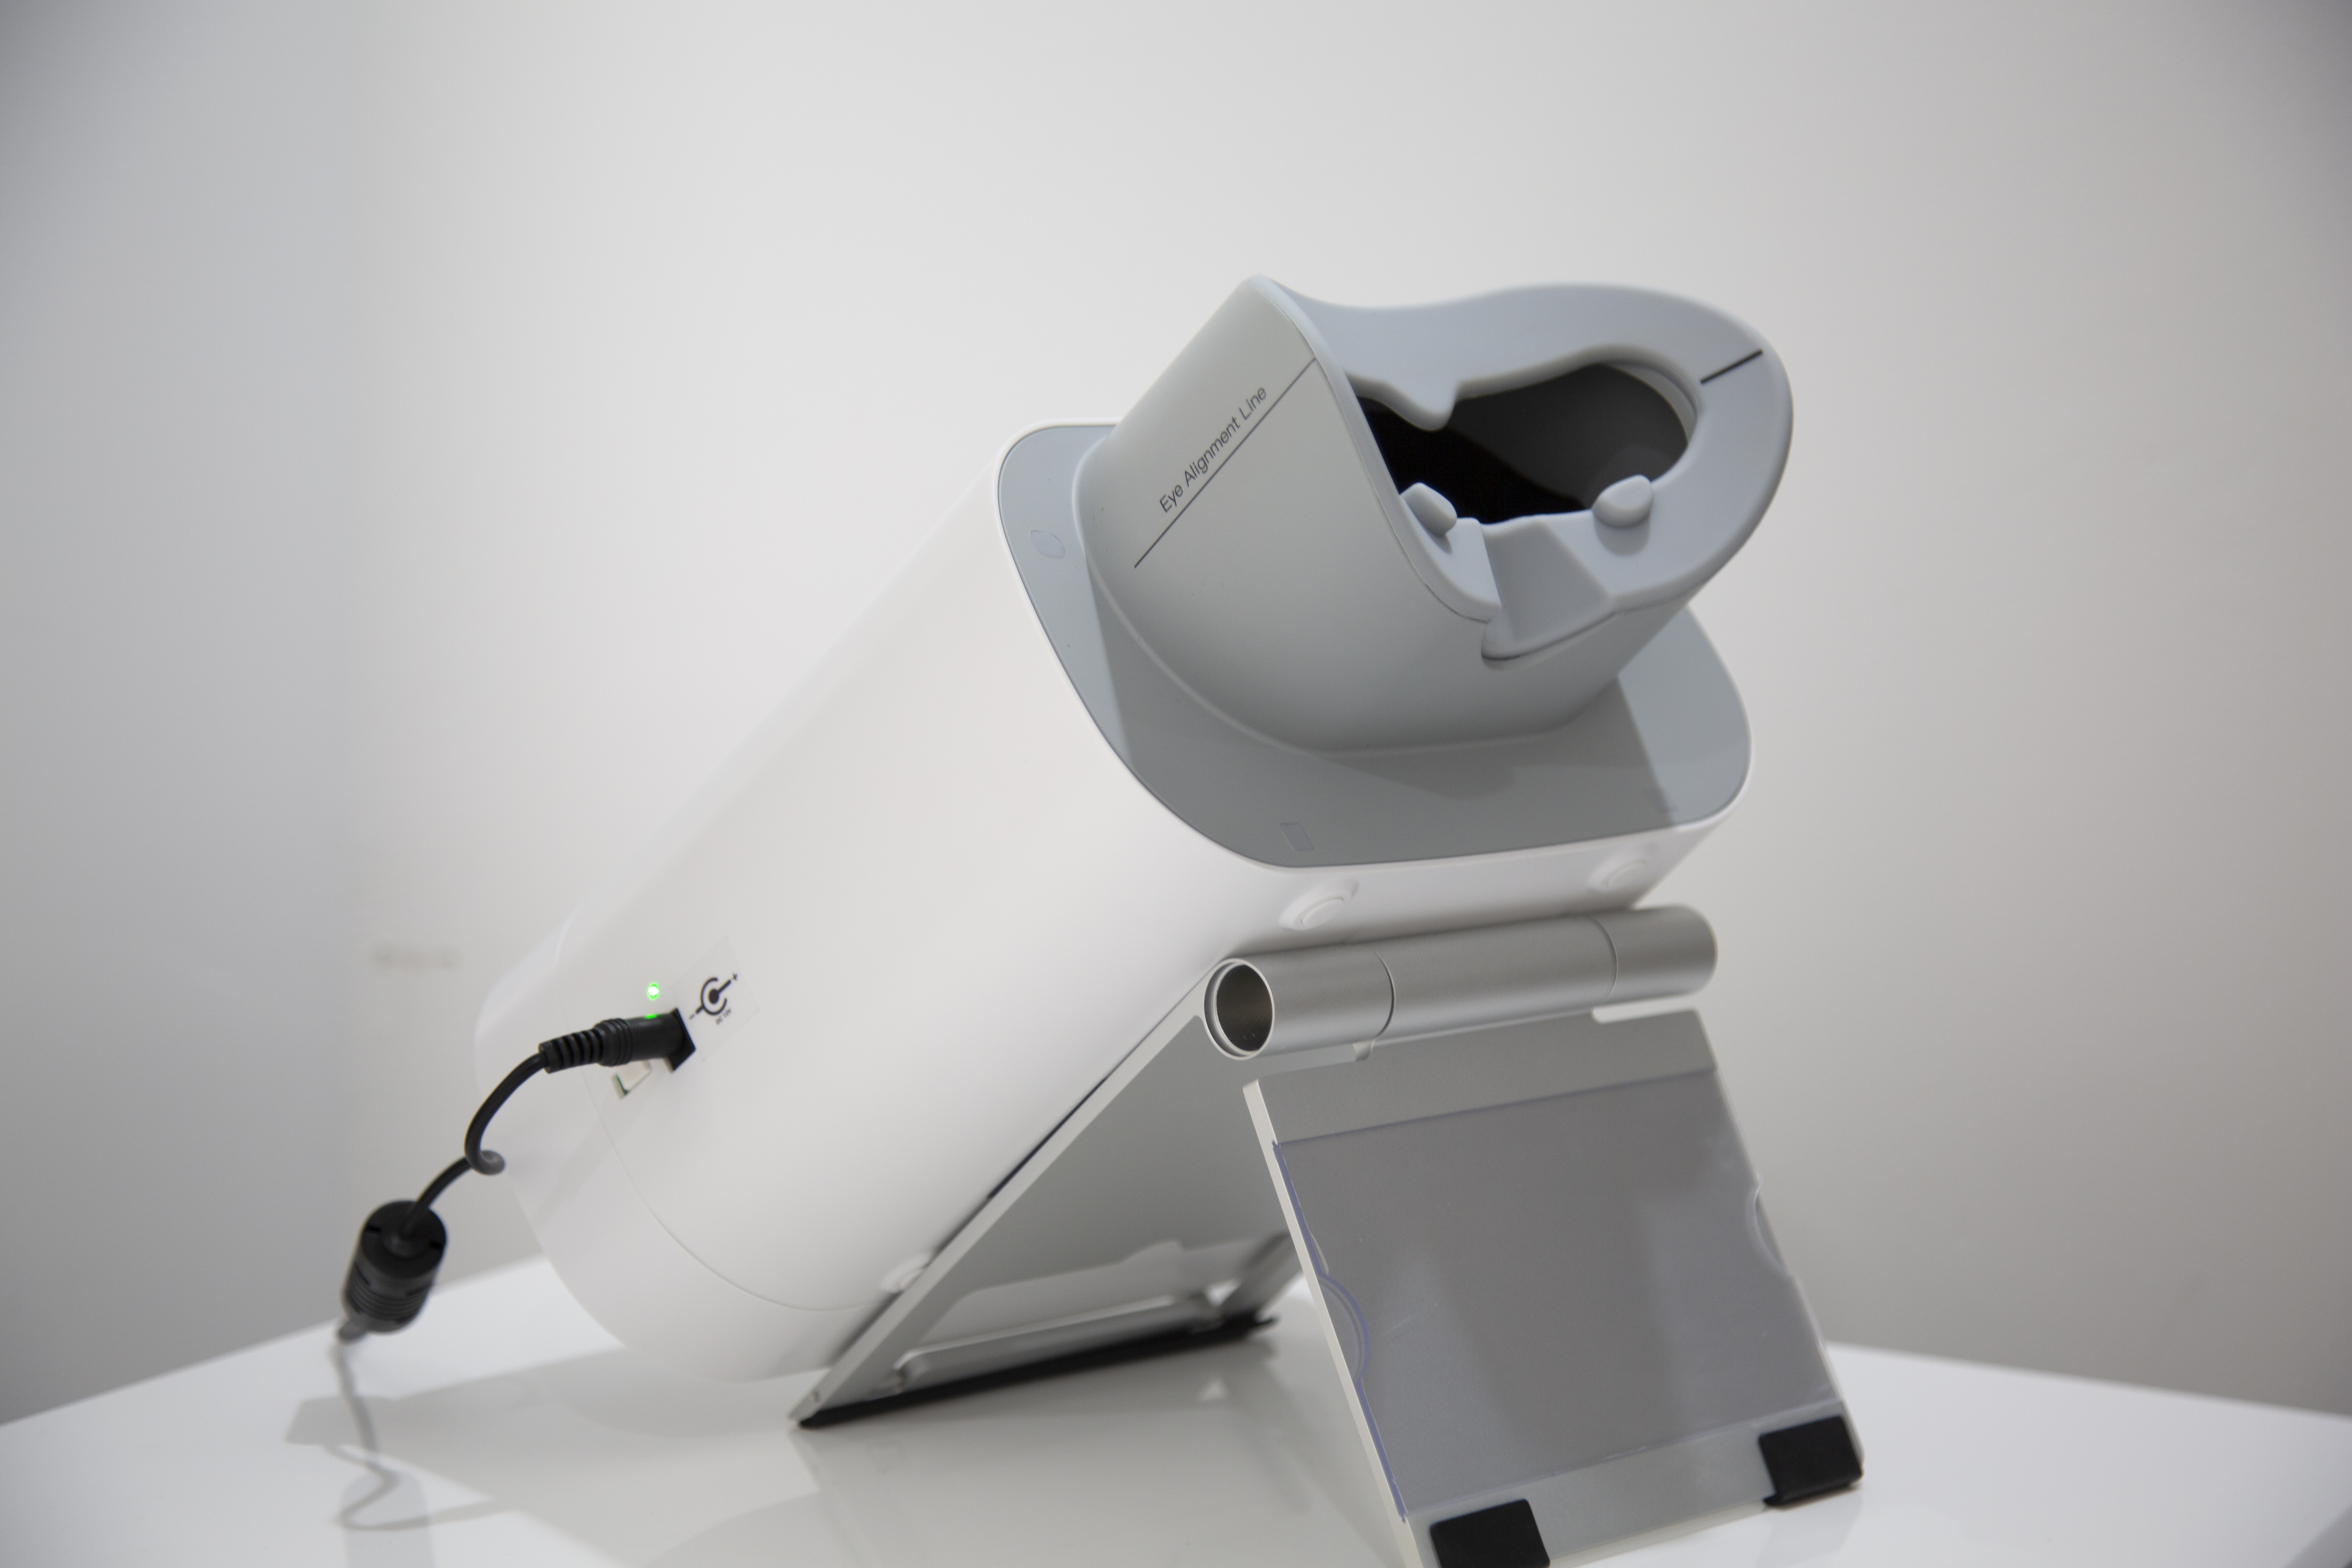
\includegraphics[keepaspectratio]{_resources/images/camera/A14A9482.jpg}}

}

\caption{The Opticare AI Fundus Camera}

\end{figure}%

\section{Initial Setup}\label{initial-setup}

\subsection{Equipment Requirements}\label{equipment-requirements}

\begin{itemize}
\tightlist
\item
  Stable table or cart
\item
  Power outlet
\item
  Reliable internet connection
\item
  (Optional) Computer or tablet with Windows 10 or higher
\item
  USB cable (provided)
\item
  Power adapter (provided)
\end{itemize}

Follow these steps to get started:

\begin{enumerate}
\def\labelenumi{\arabic{enumi}.}
\tightlist
\item
  \textbf{Unpack the Camera}: Open the case, take out the camera and the
  stand.
\end{enumerate}

\begin{figure}[H]

{\centering \pandocbounded{\includegraphics[keepaspectratio]{_resources/images/camera/CameraUnpacked.jpeg}}

}

\caption{The camera arrives in a case with all materials you'll need}

\end{figure}%

\begin{enumerate}
\def\labelenumi{\arabic{enumi}.}
\setcounter{enumi}{1}
\tightlist
\item
  \textbf{Set Up the Stand}: Unfold the stand. Ensure the QR code is
  facing front. You can take out the QR code if you choose to not
  letting the users to scan themselves.
\end{enumerate}

\begin{figure}[H]

{\centering \pandocbounded{\includegraphics[keepaspectratio]{_resources/images/camera/CameraStand.jpeg}}

}

\caption{Set up the stand with the QR code facing front}

\end{figure}%

\begin{enumerate}
\def\labelenumi{\arabic{enumi}.}
\setcounter{enumi}{2}
\tightlist
\item
  \textbf{Remove the key} The camera is locked for transportation.
  Unlock by removing the screw key located at the bottom of the device.
\end{enumerate}

\begin{figure}[H]

{\centering \pandocbounded{\includegraphics[keepaspectratio]{_resources/images/camera/CameraUnscrew.jpeg}}

}

\caption{Twist the key counter-clockwise to remove it}

\end{figure}%

\begin{tcolorbox}[enhanced jigsaw, titlerule=0mm, bottomrule=.15mm, breakable, colframe=quarto-callout-important-color-frame, leftrule=.75mm, colbacktitle=quarto-callout-important-color!10!white, left=2mm, title=\textcolor{quarto-callout-important-color}{\faExclamation}\hspace{0.5em}{Save the key!}, bottomtitle=1mm, opacityback=0, colback=white, opacitybacktitle=0.6, coltitle=black, toptitle=1mm, arc=.35mm, rightrule=.15mm, toprule=.15mm]

You will need the key when you pack the camera for transportation, so
put it in a place where you won't lose it.

\end{tcolorbox}

\textbf{Power Connection}: Connect the power adaptor and switch on the
power located on the left side of the camera. The green indication led
should be on.

\begin{figure}[H]

{\centering \pandocbounded{\includegraphics[keepaspectratio]{_resources/images/camera/CameraPowerOn.jpeg}}

}

\caption{Connect the power connector to the side of the camera}

\end{figure}%

\textbf{Initialization}: Wait for the camera to initialize and prompt
you for the next steps.

\begin{tcolorbox}[enhanced jigsaw, titlerule=0mm, bottomrule=.15mm, breakable, colframe=quarto-callout-note-color-frame, leftrule=.75mm, colbacktitle=quarto-callout-note-color!10!white, left=2mm, title=\textcolor{quarto-callout-note-color}{\faInfo}\hspace{0.5em}{Note}, bottomtitle=1mm, opacityback=0, colback=white, opacitybacktitle=0.6, coltitle=black, toptitle=1mm, arc=.35mm, rightrule=.15mm, toprule=.15mm]

The camera is pre-configured with your Wi-Fi network. You should hear
the message: ``Connected to the network,'' confirming it is connected to
your Wi-Fi. Please refer to the email for the Wi-Fi that the device is
configured with.

\end{tcolorbox}

\textbf{Unlock the Camera}: Press the larger white button on the right
side of the camera three times quickly. This unlocks the camera. There
is a lock key under the camera that needs to be unscrewed for unlocking.

\subsection{Environment Optimization}\label{environment-optimization}

\begin{itemize}
\tightlist
\item
  Room lighting: Moderate to dim
\item
  Temperature: Maintain between 5°C - 40°C
\item
  Humidity: Keep between 10\% - 90\%
\item
  Avoid direct sunlight on equipment
\item
  Ensure adequate ventilation
\end{itemize}

\bookmarksetup{startatroot}

\chapter*{References}\label{references}
\addcontentsline{toc}{chapter}{References}

\markboth{References}{References}

\phantomsection\label{refs}
\begin{CSLReferences}{1}{0}
\bibitem[\citeproctext]{ref-chua_ambient_2020}
Chua, Sharon Y. L., Anthony P. Khawaja, Andrew D. Dick, James Morgan,
Baljean Dhillon, Andrew J. Lotery, Nicholas G. Strouthidis, et al. 2020.
{``Ambient {Air} {Pollution} {Associations} with {Retinal} {Morphology}
in the {UK} {Biobank}.''} \emph{Investigative Opthalmology \& Visual
Science} 61 (5): 32. \url{https://doi.org/10.1167/iovs.61.5.32}.

\bibitem[\citeproctext]{ref-hua_development_2022}
Hua, Rong, Jianhao Xiong, Gail Li, Yidan Zhu, Zongyuan Ge, Yanjun Ma,
Meng Fu, et al. 2022. {``Development and Validation of a Deep Learning
Algorithm Based on Fundus Photographs for Estimating the {CAIDE}
Dementia Risk Score.''} \emph{Age and Ageing} 51 (12): afac282.
\url{https://doi.org/10.1093/ageing/afac282}.

\bibitem[\citeproctext]{ref-kivipelto_risk_2006}
Kivipelto, Miia, Tiia Ngandu, Tiina Laatikainen, Bengt Winblad, Hilkka
Soininen, and Jaakko Tuomilehto. 2006. {``Risk Score for the Prediction
of Dementia Risk in 20 Years Among Middle Aged People: A Longitudinal,
Population-Based Study.''} \emph{The Lancet Neurology} 5 (9): 735--41.
\url{https://doi.org/10.1016/S1474-4422(06)70537-3}.

\bibitem[\citeproctext]{ref-lin_application_2021}
Lin, Duoru, Jianhao Xiong, Congxin Liu, Lanqin Zhao, Zhongwen Li,
Shanshan Yu, Xiaohang Wu, et al. 2021b. {``Application of
{Comprehensive} {Artificial} Intelligence {Retinal} {Expert} ({CARE})
System: A National Real-World Evidence Study.''} \emph{The Lancet
Digital Health} 3 (8): e486--95.
\url{https://doi.org/10.1016/S2589-7500(21)00086-8}.

\bibitem[\citeproctext]{ref-lin_application_2021-1}
---------, et al. 2021a. {``Application of {Comprehensive} {Artificial}
Intelligence {Retinal} {Expert} ({CARE}) System: A National Real-World
Evidence Study.''} \emph{The Lancet Digital Health} 3 (8): e486--95.
\url{https://doi.org/10.1016/S2589-7500(21)00086-8}.

\bibitem[\citeproctext]{ref-ma_deep_2022}
Ma, Yanjun, Jianhao Xiong, Yidan Zhu, Zongyuan Ge, Rong Hua, Meng Fu,
Chenglong Li, et al. 2022. {``Deep Learning Algorithm Using Fundus
Photographs for 10-Year Risk Assessment of Ischemic Cardiovascular
Diseases in {China}.''} \emph{Science Bulletin} 67 (1): 17--20.
\url{https://doi.org/10.1016/j.scib.2021.08.016}.

\bibitem[\citeproctext]{ref-milea_artificial_2020}
Milea, Dan, Raymond P. Najjar, Zhubo Jiang, Daniel Ting, Caroline
Vasseneix, Xinxing Xu, Masoud Aghsaei Fard, et al. 2020. {``Artificial
{Intelligence} to {Detect} {Papilledema} from {Ocular} {Fundus}
{Photographs}.''} \emph{New England Journal of Medicine} 382 (18):
1687--95. \url{https://doi.org/10.1056/NEJMoa1917130}.

\bibitem[\citeproctext]{ref-mitani_detection_2019}
Mitani, Akinori, Abigail Huang, Subhashini Venugopalan, Greg S. Corrado,
Lily Peng, Dale R. Webster, Naama Hammel, Yun Liu, and Avinash V.
Varadarajan. 2019. {``Detection of Anaemia from Retinal Fundus Images
via Deeplearning.''} \emph{Nature Biomedical Engineering} 4 (1): 18--27.
\url{https://doi.org/10.1038/s41551-019-0487-z}.

\bibitem[\citeproctext]{ref-nusinovici_application_2024}
Nusinovici, Simon, Tyler Hyungtaek Rim, Hengtong Li, Marco Yu, Mihir
Deshmukh, Ten Cheer Quek, Geunyoung Lee, et al. 2024. {``Application of
a Deep-Learning Marker for Morbidity and Mortality Prediction Derived
from Retinal Photographs: A Cohort Development and Validation Study.''}
\emph{The Lancet Healthy Longevity}, September, 100593.
\url{https://doi.org/10.1016/S2666-7568(24)00089-8}.

\bibitem[\citeproctext]{ref-nusinovici_retinal_2022}
Nusinovici, Simon, Tyler Hyungtaek Rim, Marco Yu, Geunyoung Lee,
Yih-Chung Tham, Ning Cheung, Crystal Chun Yuen Chong, et al. 2022a.
{``Retinal Photograph-Based Deep Learning Predicts Biological Age, and
Stratifies Morbidity and Mortality Risk.''} \emph{Age and Ageing} 51
(4): afac065. \url{https://doi.org/10.1093/ageing/afac065}.

\bibitem[\citeproctext]{ref-nusinovici_retinal_2022-1}
---------, et al. 2022b. {``Retinal Photograph-Based Deep Learning
Predicts Biological Age, and Stratifies Morbidity and Mortality Risk.''}
\emph{Age and Ageing} 51 (4): afac065.
\url{https://doi.org/10.1093/ageing/afac065}.

\bibitem[\citeproctext]{ref-tsukahara_is_2021}
Tsukahara, Jason S., and Randall W. Engle. 2021. {``Is Baseline Pupil
Size Related to Cognitive Ability? {Yes} (Under Proper Lighting
Conditions).''} \emph{Cognition} 211 (June): 104643.
\url{https://doi.org/10.1016/j.cognition.2021.104643}.

\bibitem[\citeproctext]{ref-wong_retinal_2002}
Wong, Tien Yin. 2002. {``Retinal {Arteriolar} {Narrowing} and {Risk} of
{Diabetes} {Mellitus} in {Middle}-Aged {Persons}.''} \emph{JAMA} 287
(19): 2528. \url{https://doi.org/10.1001/jama.287.19.2528}.

\bibitem[\citeproctext]{ref-xia_generalizing_2024}
Xia, Peng, Ming Hu, Feilong Tang, Wenxue Li, Wenhao Zheng, Lie Ju, Peibo
Duan, Huaxiu Yao, and Zongyuan Ge. 2024. {``Generalizing to {Unseen}
{Domains} in {Diabetic} {Retinopathy} with {Disentangled}
{Representations}.''} arXiv. \url{http://arxiv.org/abs/2406.06384}.

\bibitem[\citeproctext]{ref-zhao_foundation_2024}
Zhao, Theodore, Yu Gu, Jianwei Yang, Naoto Usuyama, Ho Hin Lee, Sid
Kiblawi, Tristan Naumann, et al. 2024. {``A Foundation Model for Joint
Segmentation, Detection and Recognition of Biomedical Objects Across
Nine Modalities.''} \emph{Nature Methods}, November.
\url{https://doi.org/10.1038/s41592-024-02499-w}.

\bibitem[\citeproctext]{ref-zhu_retinal_2023}
Zhu, Zhuoting, Danli Shi, Peng Guankai, Zachary Tan, Xianwen Shang,
Wenyi Hu, Huan Liao, et al. 2023. {``Retinal Age Gap as a Predictive
Biomarker for Mortality Risk.''} \emph{British Journal of Ophthalmology}
107 (4): 547--54.
\url{https://doi.org/10.1136/bjophthalmol-2021-319807}.

\end{CSLReferences}


\backmatter


\end{document}
